% Chapter 14
%\chapter{Consolidation processes}
%\textit{by Joshua Taron, Norihiro Watanabe, Wenqing Wang}

The purpose of the benchmarks in this chapter is to test the validity of coupled hydro-mechanical (HM) and two-phase hydro-mechanical (H$^2$M) processes. Mechanical compression generates a fluid pressure response, while pressure storage and dissipation modify the mechanical condition via the effective stress. The tests we use are convenient and fundamental validations of the deformation and flow modules, most importantly guaranteeing that the coupling is correct between them. 

We examine real systems, where fluids, solids, and solid grains are compressible. In the single phase case, comparisons are made between two finite element coupling schemes: 1) Monolithic: solid and fluid equations solved in a single matrix and 2) Staggered: solid and fluid equations solved iteratively. Two-phase flow consolidation is also examined and then an adapted form of extended finite elements (XFEM) is used to observe the fluid-mechanical interaction in a discrete fracture-matrix system. 

%.........................................................................
%\section{Single Phase}
\section{Single phase consolidation}
Let us begin by introducing a few governing equations.

\subsubsection*{Fluid mass and momentum balance}
Linear momentum balance for the fluid follows Darcy:

\begin{equation}
{v}_{ri}=\phi \left( {{v}_{i}}-{{v}_{si}} \right)=-\frac{{{k}_{ij}}}{\mu }\left( \frac{\partial p}{\partial {{x}_{j}}}+\rho {{g}_{j}} \right),
\label{eqch14:genmass}
\end{equation}

for the intrinsic permeability, ${{k}_{ij}}$, dynamic viscosity, $\mu $, and density, $\rho $. The subscript $r$ considers that fluid velocity is relative to motion of the deformable solid (${{v}_{si}}$), so that ${{v}_{i}}$ is absolute fluid velocity, and ${{v}_{ri}}$ is relative. Conservation of fluid mass requires,

\begin{equation}
\frac{\partial }{\partial t}\left( \phi \rho  \right)+\frac{\partial }{\partial {{x}_{i}}}\left( \phi \rho {{v}_{i}} \right)=0.
\end{equation}
	
Fluid properties are functions of temperature and pressure. The fluid density time derivative appearing in the mass balance equation may be expanded to

\begin{equation}
\frac{d\rho}{dt}=\rho \left( \frac{1}{K_{f}^{p}}\frac{dp}{dt}-\frac{1}{K_{f}^{T}}\frac{dT}{dt} \right),
\end{equation}
	
with fluid compressibility given by $1/K_{f}^{p}={{\left. \left( 1/\rho  \right)\left( \partial \rho /\partial p \right) \right|}_{T}}$ and for the fluid thermal expansion coefficient $1/K_{f}^{T}=-{{\left. \left( 1/\rho  \right)\left( \partial \rho /\partial T \right) \right|}_{p}}$. In these definitions we utilize moduli ($K$ = inverse compressibility). Also, because thermal effects are not considered in these examples, the temperature dependence may be neglected. Utilizing the Lagrangian total derivative of a component relative to the moving solid, ${{d}_{s}}/dt=\partial /\partial t+{{v}_{si}}\partial /\partial {{x}_{i}}$, and a moving fluid, ${{d}_{f}}/dt=\partial /\partial t+{{v}_{fi}}\partial /\partial {{x}_{i}}$, substituting for absolute fluid velocity and dividing through by density gives,

\begin{equation}
\phi \left( \frac{1}{K_{f}^{p}}\frac{dp}{dt}+\frac{{{d}_{s}}\phi }{dt}+\frac{\partial {{v}_{si}}}{\partial {{x}_{i}}} \right)=-\frac{\partial }{\partial {{x}_{i}}}\left( {{v}_{ri}} \right).
\end{equation}
	
To obtain the porosity time derivative, we expand the solid mass balance to obtain

\begin{equation}
\frac{{{d}_{s}}\phi }{dt}=\frac{\left( 1-\phi  \right)}{{{\rho }_{s}}}\frac{\partial {{\rho }_{s}}}{\partial t}+\left( 1-\phi  \right)\frac{\partial {{v}_{si}}}{\partial {{x}_{i}}}.
\end{equation}
	
Substituting this gives,

\begin{equation}
\frac{\phi }{K_{f}^{p}}\frac{dp}{dt}+\left[ \frac{\partial {{v}_{si}}}{\partial {{x}_{i}}}+\frac{\left( 1-{{\rho }_{s}} \right)}{{{\rho }_{s}}}\frac{\partial {{\rho }_{s}}}{\partial t} \right]=-\frac{\partial }{\partial {{x}_{i}}}\left( {{v}_{ri}} \right).
\end{equation}
	
Utilizing Biot's formulation to represent the solid density time derivative and assuming small strain yields the full fluid mass balance (\cite{KhaliliSelvadurai:03} and \cite{RutEtAl:01}),

\begin{equation}
\left( \frac{\phi }{K_{f}^{p}}+\overbrace{\frac{\left( \alpha -\phi  \right)}{{{K}_{g}}}}^{A} \right)\frac{dp}{dt}+\overbrace{\alpha \frac{\partial {{v}_{si}}}{\partial {{x}_{i}}}}^{B}=-\frac{\partial }{\partial {{x}_{i}}}\left( {{v}_{ri}} \right),
\label{eqch14:flmass}
\end{equation}
	
where ${{K}_{g}}$ is the solid grain bulk modulus, and $\alpha$ is the Biot-Willis coefficient ($\alpha =1-K/{{K}_{g}}$ in an ideal, fully interconnected porous media). The bracketed terms $A$ and $B$ represent important couplings from the mechanical system to that of the fluid. All are vital in the HM procedure and without them the equation simplifies to a standard fluid flow equation with fluid compressibility storage in the pressure time derivative. 

\subsubsection*{Solid momentum balance}

We begin with the concept of effective stress,

\begin{equation}
\sigma {{'}_{ij}}={{\sigma }_{ij}}+\alpha p{{\delta }_{ij}},
\end{equation}

for the effective stress, $\sigma '$, and the total stress, $\sigma$; negative in compression. Balance of linear momentum is defined by,

\begin{equation}
\frac{\partial {{\sigma }_{ij}}}{\partial {{x}_{j}}}+{{F}_{i}}=0,
\end{equation}

for the body force, $F=\rho _m \text{g}$ and where $\rho _m =\phi \rho _f + (1-\phi )\rho _s$ is density of the mixture. From the definition of strain, ${{\varepsilon }_{ij}}=\left( \partial {{u}_{i}}/\partial {{x}_{j}}+\partial {{u}_{j}}/\partial {{x}_{i}} \right)/2$, and an arbitrary stress-strain relationship of the form $\mathbf{\sigma }=\mathbf{D\varepsilon }\left( \mathbf{u} \right)$, we write the displacement formulation of mechanical equilibrium (neglecting thermal effects) for isotropic linear elasticity,

\begin{equation}
\frac{\partial }{\partial {{x}_{j}}}\left[ G\frac{\partial {{u}_{i}}}{\partial {{x}_{j}}}+\left( \lambda +G \right)\frac{\partial {{u}_{j}}}{\partial {{x}_{i}}}-\alpha p{{\delta }_{ij}} \right]+{{F}_{i}}=0,
\label{eqch14:mequil}
\end{equation}

where $G$ and $\lambda$ are the Lam� constants. Changes to the fluid system are therefore visited in mechanical equilibrium via the effective stress.

\subsubsection*{Numerical solution scheme}
The numerical solution of Eqs. \ref{eqch14:flmass} and \ref{eqch14:mequil} can be obtained with any convenient method. In these benchmarks, we use a standard Galerkin finite element spatial discretization with time discretization following a generalized first order finite difference scheme, as implemented in OpenGeoSys. Note that Eq. \ref{eqch14:mequil} is an equilibrium equation, and has no time dependency other than that imposed by coupling terms to fluid behavior. The result is a set of coupled linear equations in pressure, $p$, and solid displacement, $u$. The two equations may be solved sequentially and iteratively, or monolithically as a single system. We present results using both solution schemes in the following benchmarks.

%-------------------------------------------------------------------------
%-------------------------------------------------------------------------

\subsection{Background}
\subsubsection*{Mass balance equation}
Consider two-phase flow in porous media, e.g liquid (denoted by $l$) and gas (denoted by $g$). For each phase in two-phase fluid flow, mass conservation is given by the following equation:

\begin{align}
\pD{}{t}\left(\poro S^g\dens_k^g+\poro S^l\dens_k^l\right)+\nabla \cdot \left( \FlxDf_k^g+\FlxDf_k^l\right)=Q_k
\label{eq:massb}
\end{align}

where $S$ is saturation, $\dens$ stands for phase density, $\poro$ is the porosity, $\FlxDf$ is total flux. The subscript $k$ in equation (\ref{eq:massb}) denotes the component, e.g air ($k=a$) or water ($k=w$), within each phase, $\gamma=(g,l)$. For any phase $\gamma=(g,l)$, an advection vector ${{\FlxDf}_A}_k^{\gamma}$ and a diffusion vector  ${{\FlxDf}_D}_k^{\gamma}$ comprise the total flux, i.e

\begin{align}
\FlxDf_k^{\gamma}={{\FlxDf}_A}_k^{\gamma}+{{\FlxDf}_D}_k^{\gamma}
\label{eq:tflx}
\end{align}

According to Darcy's law, the advective part of the total flux may be written as

\begin{align}
{{\FlxDf}_A}_k^{\gamma}=-\dens_k^{\gamma}\dfrac{\perm \RelKa^{\gamma}}{\mu^{\gamma}}\left(\nabla \pres^{\gamma}-\dens^{\gamma} \mathbf g\right)
\label{eq:flx_dc}
\end{align}

where $\perm$ is the intrinsic permeability, $\RelKa^{\gamma}$ is the relative permeability of the phase, and $\mu^{\gamma}$ is the viscosity.

The diffusive part of the total flux is given by Fick's law

\begin{align}
{{\FlxDf}_D}_k^{\gamma}=-\poro \sat^{\gamma}  \dens^{\gamma} {\mathbb D}_k^{\gamma} \nabla \left(\dfrac{\dens_k^{\gamma}}{\dens^{\gamma}}\right)
\label{eq:flx_fk}
\end{align}

where $\mathbb D$ is the diffusion coefficient tensor. Since $\dens^{\gamma} = \dens_a^{\gamma}+\dens_w^{\gamma}$, we have

 \begin{align}
{{\FlxDf}_D}_w^{\gamma}+{{\FlxDf}_D}_a^{\gamma}=\mathbf 0
\label{eq:dufblc}
\end{align}

under the assumption ${\mathbb D}_a^{\gamma}  = {\mathbb D}_w^{\gamma} $.

Consider a water-air mixture. We expand the mass balance equation (\ref{eq:massb}) with the flux defined in equations (\ref{eq:tflx}) based upon the above equations (\ref{eq:tflx}, \ref{eq:flx_dc}, \ref{eq:flx_fk}). For the water component, the diffusive part of the total flux takes the form

\begin{align}
{{\FlxDf}_D}_w^{l}=-\poro \Sat^{l}  \dens^{l} {\mathbb D}_w^{l} \nabla \left(\dfrac{\dens_w^{l}}{\dens^{l}}\right),\quad
{{\FlxDf}_D}_w^{g}=-\poro \Sat^{g}  \dens^{g} {\mathbb D}_w^{g} \nabla \left(\dfrac{\dens_w^{g}}{\dens^{g}}\right)
\label{eq:flx_fkw}
\end{align}

Obviously, ${\mathbb D}_w^{l} = \mathbf 0$. Therefore, the mass balance equation for water component can be written as follows

\begin{align}
\pD{}{t} \left(\poro S^g\dens_w^g+\poro S^l\dens_w^l\right)-
\nabla \cdot \left[\dens_w^{l}\dfrac{\perm \RelKa^{l}}{\mu^{l}}\left(\nabla \pres^{l}-\dens^{l} \mathbf g\right)\right]\nonumber\\
-\nabla \cdot \left[\dens_w^{g}\dfrac{\perm \RelKa^{g}}{\mu^{g}}\left(\nabla \pres^{g}-\dens^{g} \mathbf g\right)\right] -
\nabla \cdot \left[\poro \Sat^{g}  \dens^{g} {\mathbb D}_w^{g} \nabla \left(\dfrac{\dens_w^{g}}{\dens^{g}}\right)\right] = Q_w
\label{eq:massblq}
\end{align}

Since the capillary pressure $\pres^c$  is chosen as one of the two unknowns of equation (\ref{eq:massb}) and $S^g=1-S^l$, equation (\ref{eq:massblq}) becomes

\begin{align}
\poro (\dens_w^l -\dens_w^g)\pD{S^l}{t} +(1 -S^l)\poro \pD{\dens_w^{g}}{t} -
\nabla \cdot \left[\dens_w^{l}\dfrac{\perm \RelKa^{l}}{\mu^{l}}\left(\nabla (\pres^{g}-\pres^{c}) -\dens^{l} \mathbf g\right)\right]\nonumber\\
-\nabla \cdot \left[\dens_w^{g}\dfrac{\perm \RelKa^{g}}{\mu^{g}}\left(\nabla \pres^{g}-\dens^{g} \mathbf g\right)\right] -
\nabla \cdot \left[\poro \Sat^{g}  \dens^{g} {\mathbb D}_w^{g} \nabla \left(\dfrac{\dens_w^{g}}{\dens^{g}}\right)\right] = Q_w
\label{eq:msblq}
\end{align}

Similar to the previous procedure, the diffusion part of the total flux of air component can be written as

\begin{align}
{{\FlxDf}_D}_a^{l}=-\poro \Sat^{l}  \dens^{l} {\mathbb D}_a^{l} \nabla \left(\dfrac{\dens_a^{l}}{\dens^{l}}\right),\quad
{{\FlxDf}_D}_a^{a}=-\poro \Sat^{g}  \dens^{g} {\mathbb D}_a^{g} \nabla \left(\dfrac{\dens_a^{g}}{\dens^{g}}\right)
\label{eq:flx_fka}
\end{align}

The density shift from air component to liquid ${\dens_a^{l}}$ is very small and can be omitted. Therefore, we can assume ${{\FlxDf}_D}_a^{l}\thickapprox0$. As a consequence, the mass balance equation for air component is derived as:

$$\pD{}{t} \left(\poro S^g\dens_a^g\right) -$$
\begin{align}
\nabla \cdot \left[\dens_a^{g}\dfrac{\perm \RelKa^{g}}{\mu^{g}}\left(\nabla \pres^{g}-\dens^{g} \mathbf g\right)\right]-\nabla \cdot \left[\poro \Sat^{g}  \dens^{g} {\mathbb D}_a^{g} \nabla \left(\dfrac{\dens_a^{g}}{\dens^{g}}\right)\right] =Q_a
\label{eq:massba}
\end{align}

Expanding the temporary derivative term of equation (\ref{eq:massba}) yields

$$-\poro \dens_a^g \pD{S^l}{t} + (1 -S^l)\poro \pD{\dens_a^{g}}{t}-$$
\begin{align}
\nabla \cdot \left[\dens_a^{g}\dfrac{\perm \RelKa^{g}}{\mu^{g}}\left(\nabla \pres^{g}-\dens^{g} \mathbf g\right)\right] -
\nabla \cdot \left[\poro \Sat^{g} \dens^{g} {\mathbb D}_a^{g} \nabla \left(\dfrac{\dens_a^{g}}{\dens^{g}}\right)\right] = Q_a
\label{eq:msba}
\end{align}

The mass balance equations (\ref{eq:msblq}) and (\ref{eq:msba}) are exactly the same as described in \cite{SanPesSch:06}.

\subsubsection*{Pressure-pressure (pp) scheme}
Based on the description of isothermal two-phase flow above, (\ref{eq:msblq}) and (\ref{eq:msba}) can be modified in order to obtain governing equation for the isothermal two-phase flow in a porous medium. In this formulation primary variables are gas pressure $\asup{\pres}{g}$, and capilary pressure $\asup{\pres}{c}$.

The basic equations of the isothermal two-phase flow system are:

\begin{align}
\poro \dens_w \pD{S_w}{\pres_c} \dot\pres_c +
\nabla \cdot\left[\dens_w\dfrac{{\perm \RelKa}_{w}}{\mu_w}\left(-\nabla \pres^{g} +
\nabla{\pres}^{c} + \dens_w \mathbf g\right)\right] = Q_w
\end{align}
\begin{align}
- \poro \dens^a \pD{S_w}{\pres_c} \dot\pres_c+
\poro (1 -S_w)\left(\pD{\dens_a}{\pres^g}\dot\pres^g+\pD{\dens_a}{\pres_c}\dot\pres_c\right)+ \nonumber\\
\nabla \cdot \left[\dens_a\dfrac{{\perm \RelKa}_a}{\mu_a} \left(-\nabla\pres^{g} + \dens_a \mathbf g\right) \right] = Q_a
\label{eq:msbl_sim}
\end{align}

\subsubsection*{Pressure-saturation (pS) scheme}
Based on the description of the isothermal two-phase flow above, (\ref{eq:msblq}) and (\ref{eq:msba}) can be modified in order to obtain governing equation for the isothermal two-phase system. Primary variables of this formulation are wetting phase pressure $p_w$, and non-wetting phase saturation $S_{nw}$. The equations are simply algebraic manipulations of those in the previous section.
\subsection{Distributed footing: Poroelastic cube (3D)}
We consider a vertical cross-section through homogeneous soil. Due to symmetry we can limit the investigation to half of the domain. The model domain is then extending 8 meters in length and 5 meters in height. The problem is solved in 2D and 3D space, respectively.

\begin{figure}[!tbh]
\begin{center}
\scalebox{1.0} % Change this value to rescale the drawing.
{
\begin{picture}(380,190)
\put(70,160){\line(1,0){240}}
\put(310,10){\line(0,1){150}}
\multiput(70,10)(0,11){14}{\line(0,1){7}}
\put(75,180){\vector(0,-1){20}}
\put(80,180){\vector(0,-1){20}}
\put(85,180){\vector(0,-1){20}}
\put(90,180){\vector(0,-1){20}}
\put(95,180){\vector(0,-1){20}}
\put(308,165){8}
\put(60,165){0}
\put(55,8){-5}
% BC
% left
\put(5,100){$\frac{\partial p}{\partial x} = 0$}
\put(5,85) {$u_x = 0$}
\put(5,75) {$\sigma_{xy} = 0$}
% top
\put(75,150){$\sigma_{yy}=\sigma_0$}
\put(75,140){$\sigma_{xy}=0$}
\put(180,165){$\sigma_{xy}=\sigma_{yy}=0$}
\put(210,187){\vector(1,0){100}}
\put(175,187){\vector(-1,0){105}}
\put(180,185){$p=0$}
% right
\put(320,100){$\frac{\partial p}{\partial x} = 0$}
\put(320,85) {$u_x = 0$}
\put(320,75) {$\sigma_{xy} = 0$}
% bottom
\put(160,-5){$\frac{\partial p}{\partial y} = 0$ , $u_x=u_y=0$}
\linethickness{2pt}
\put(70,10){\line(1,0){240}}
\end{picture}
}
\end{center}
\caption{Conceptualization of the footing problem. Properties are Young's modulus, $E=3\times 10^{4}$ $N/m^{2}$, Poisson's ratio, $\nu =0.2$, permeability, $k=10^{-10}$ $m^2$, and fluid viscosity, $\mu =10^{-3}$ $Pa\,s$.}
\label{fig-setting}
\end{figure} 

\subsubsection*{Definition}
A strip loading is imposed ($\sigma _{yy}=\sigma _0$ in $x\in [0,1]$), with zero stresses
($\sigma _{yy}=\sigma _{xy}=0$ in $x\in(1,8]$) and zero pressure at the top; no horizontal flux, no horizontal displacements and zero shear stresses at left and right boundaries with no vertical flux and no displacement at the bottom (Fig. \ref{fig-setting}). 

\subsubsection*{Results}
The 3D geometry expands the 2D domain by extruding the 2D shape by 1m in the off-plane direction (\ref{fig_HM3}). Results at the critical step, i.e., the first step, are shown in Fig. \ref{fig:e10}, \ref{fig:e12} and  \ref{fig:e11}. The results produced using the 2D model with triangular elements and the 3D model with tetrahedral elements match each other well, thus providing confidence in higher dimensions.

\begin{figure}[!tbh]
\vspace{-1cm}
\begin{center}
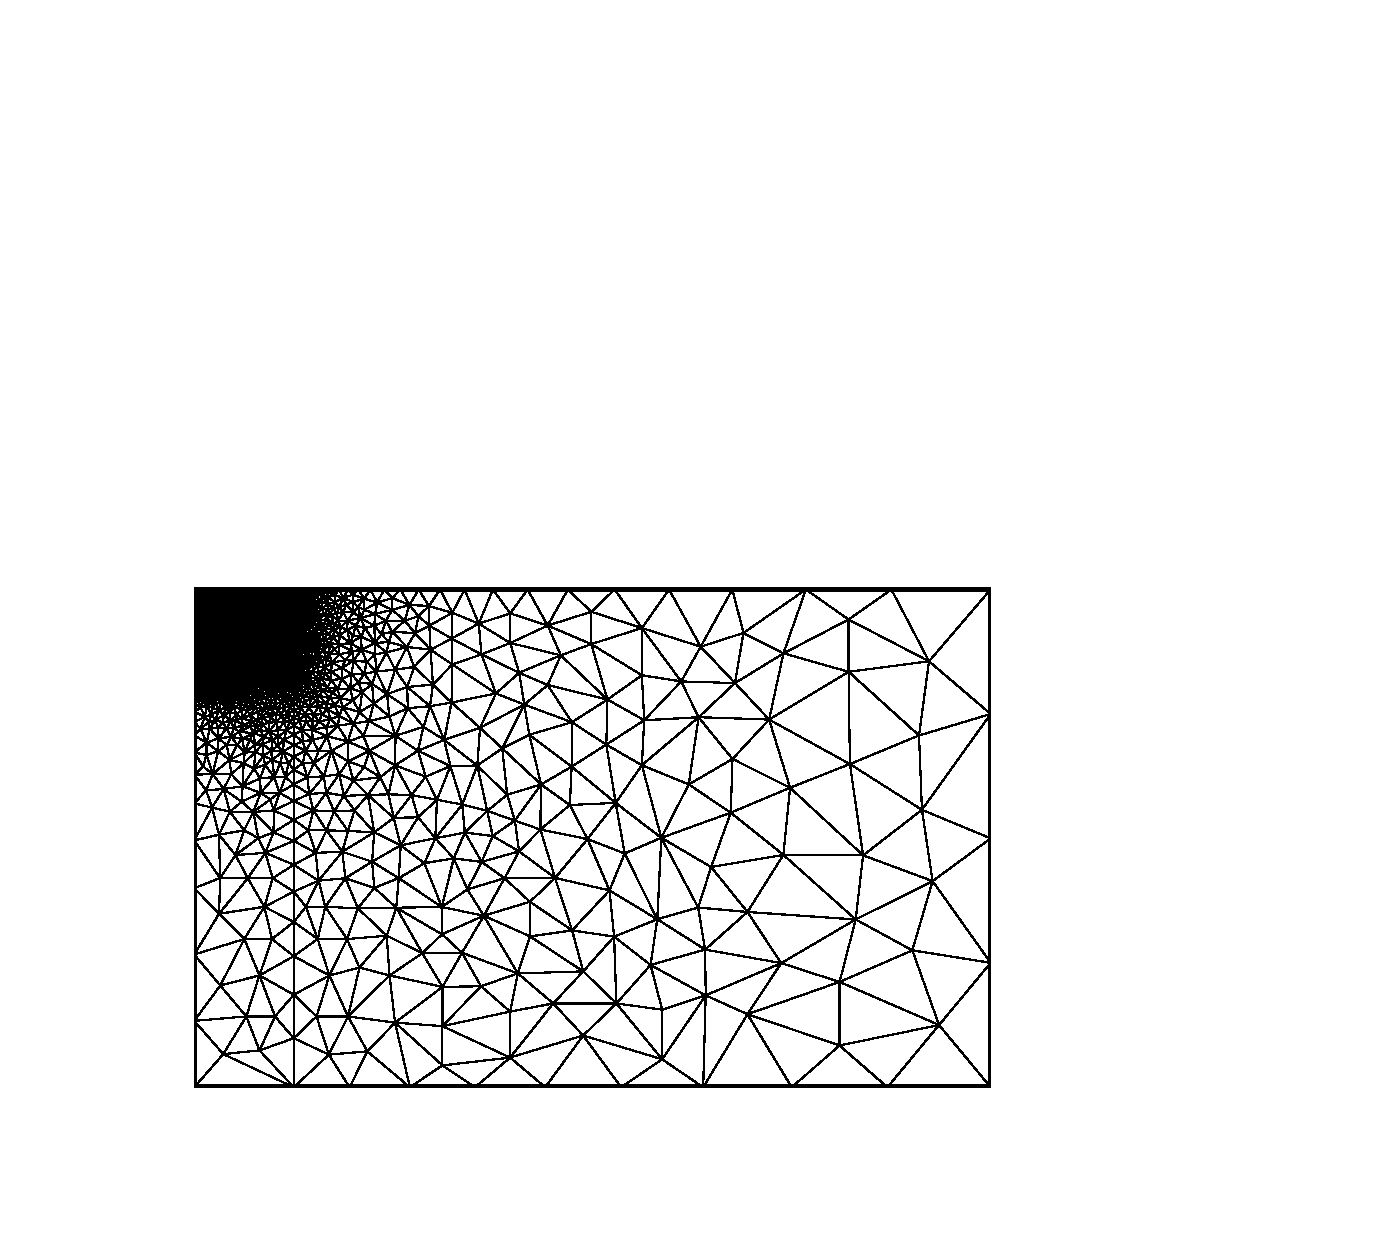
\includegraphics[width=0.54\textwidth]{chapter_14/figures/fig_14_1_4_a}
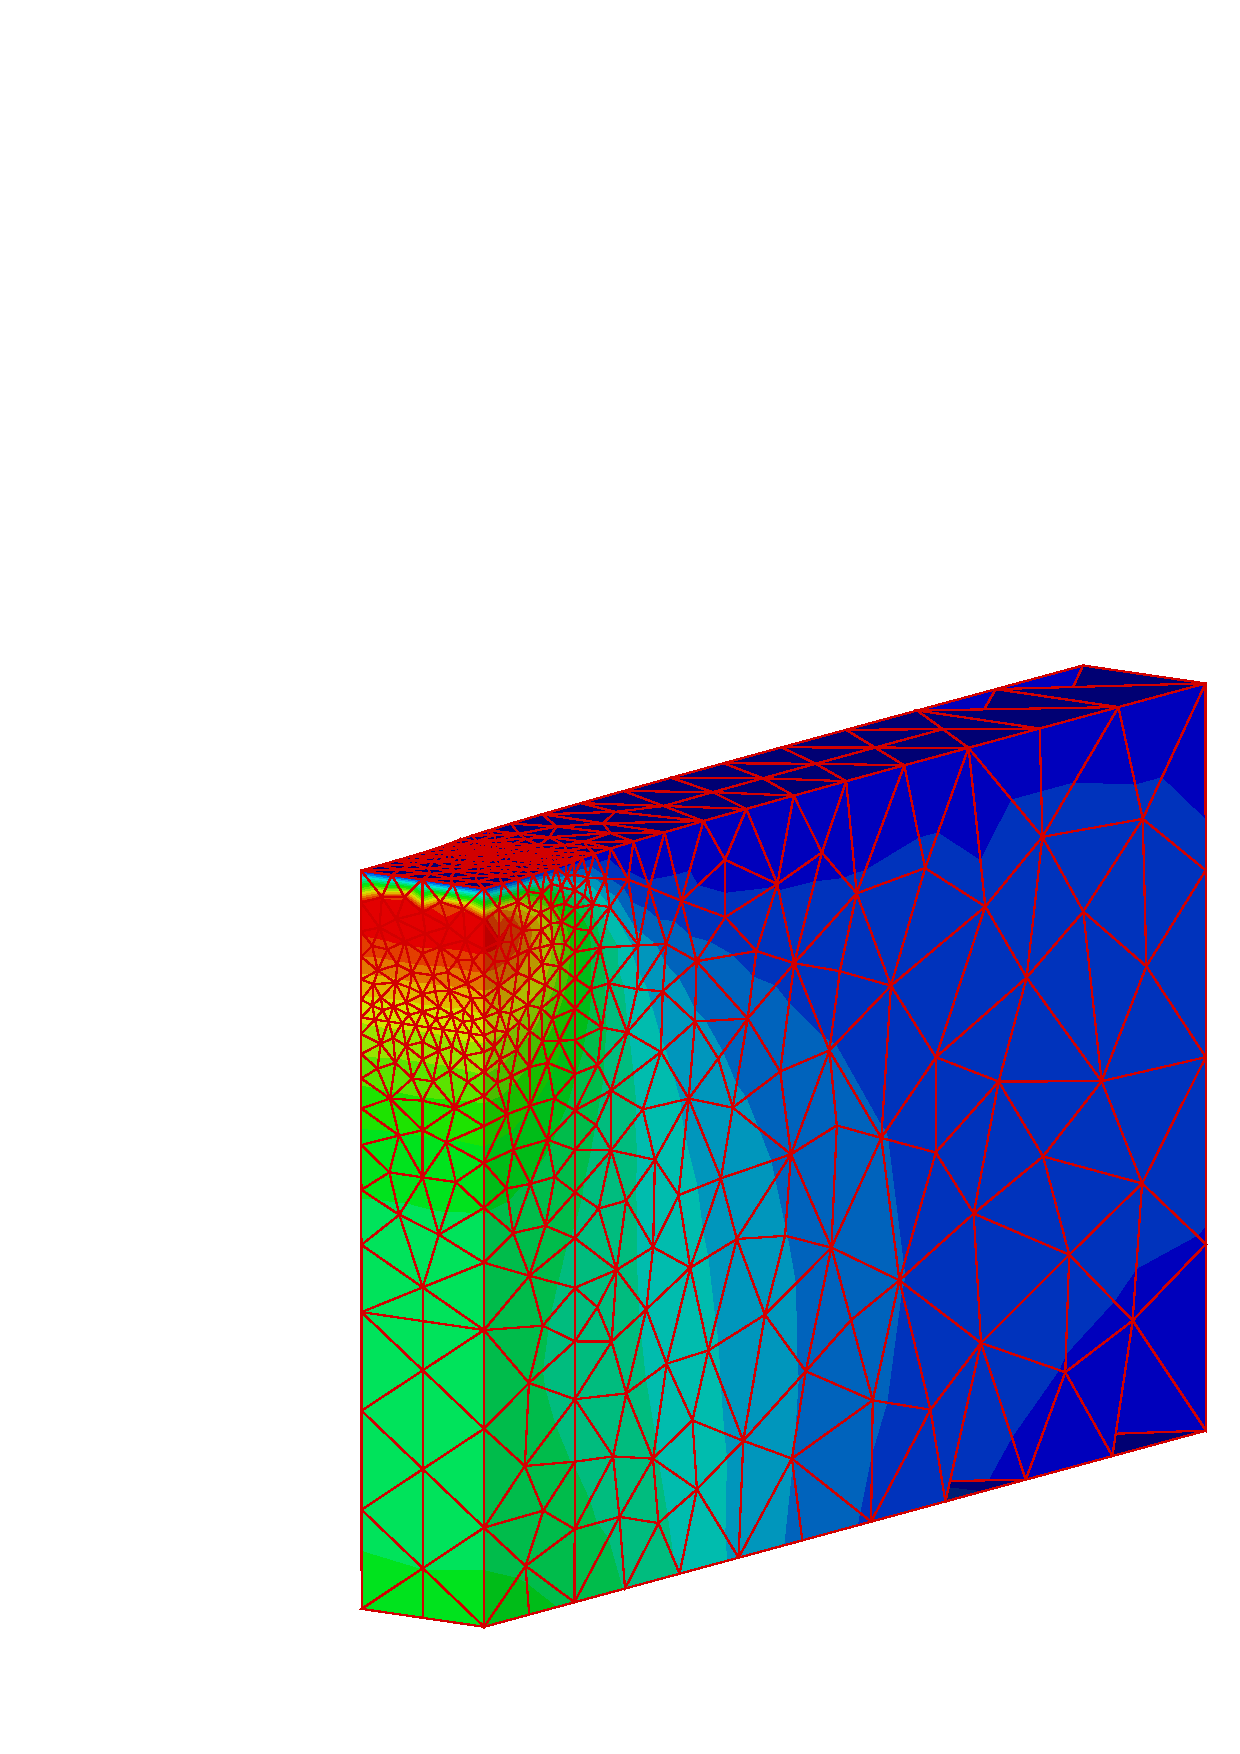
\includegraphics[width=0.44\textwidth]{chapter_14/figures/fig_14_1_4_b}
\end{center}
\vspace{-0.5cm}
\caption{Mesh geometry.}
\label{fig_HM3}
%\vspace{-1.0cm}
\end{figure}

\begin{figure}[!tbh]
\begin{center}
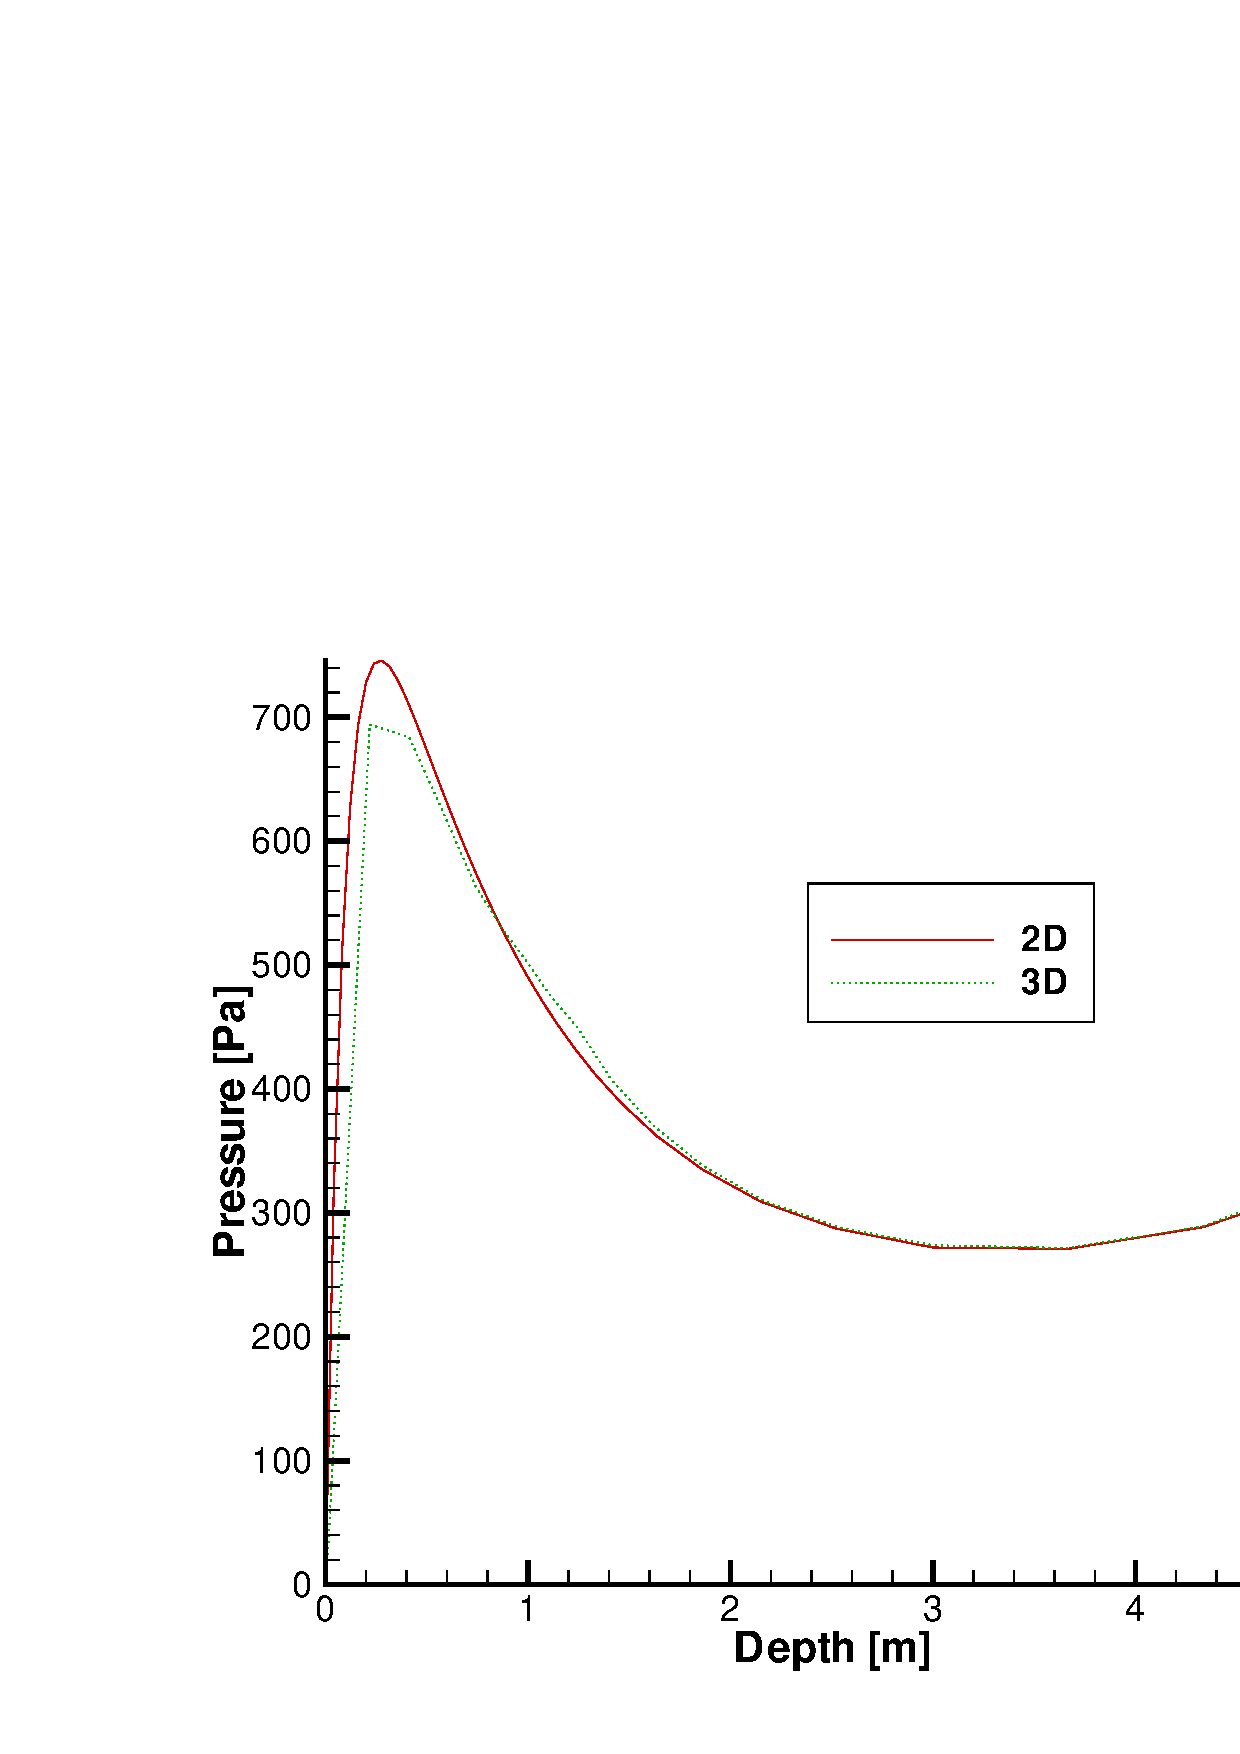
\includegraphics[width=0.49\textwidth]{chapter_14/figures/fig_14_1_5_a}
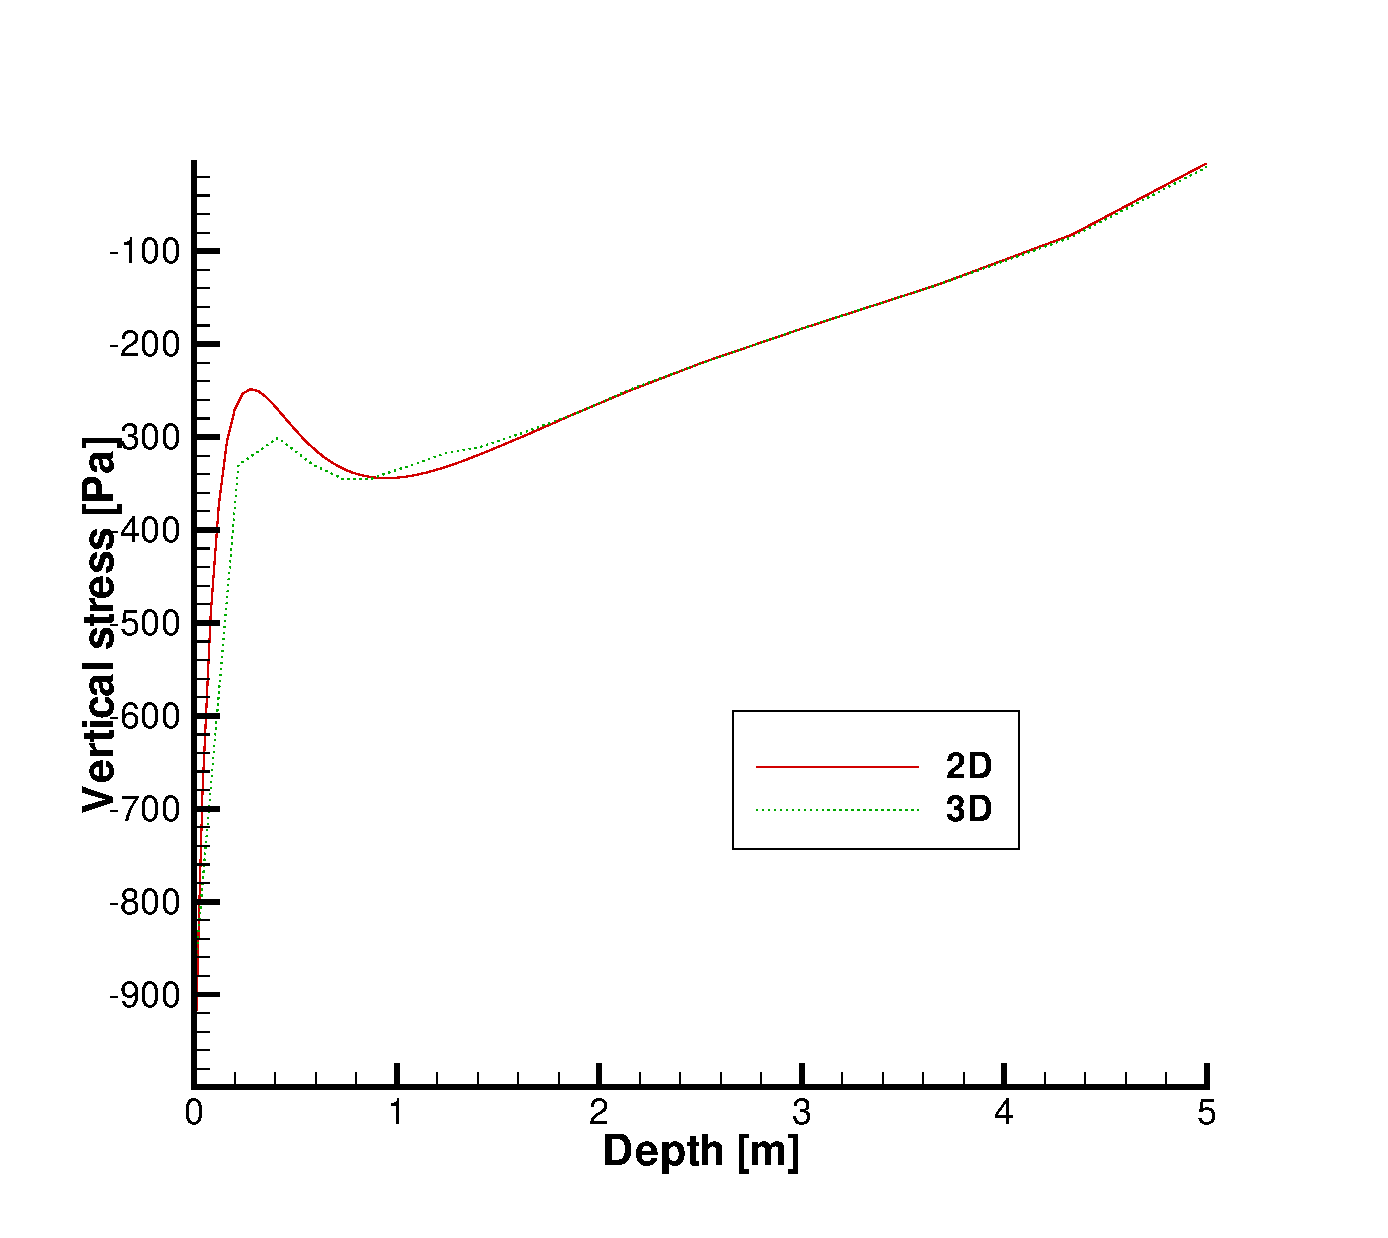
\includegraphics[width=0.49\textwidth]{chapter_14/figures/fig_14_1_5_b}
\end{center}
\caption{Comparison along symmetric axis.}  
\label{fig:e11}
\end{figure}

\begin{figure}[!tbh]
\begin{center}
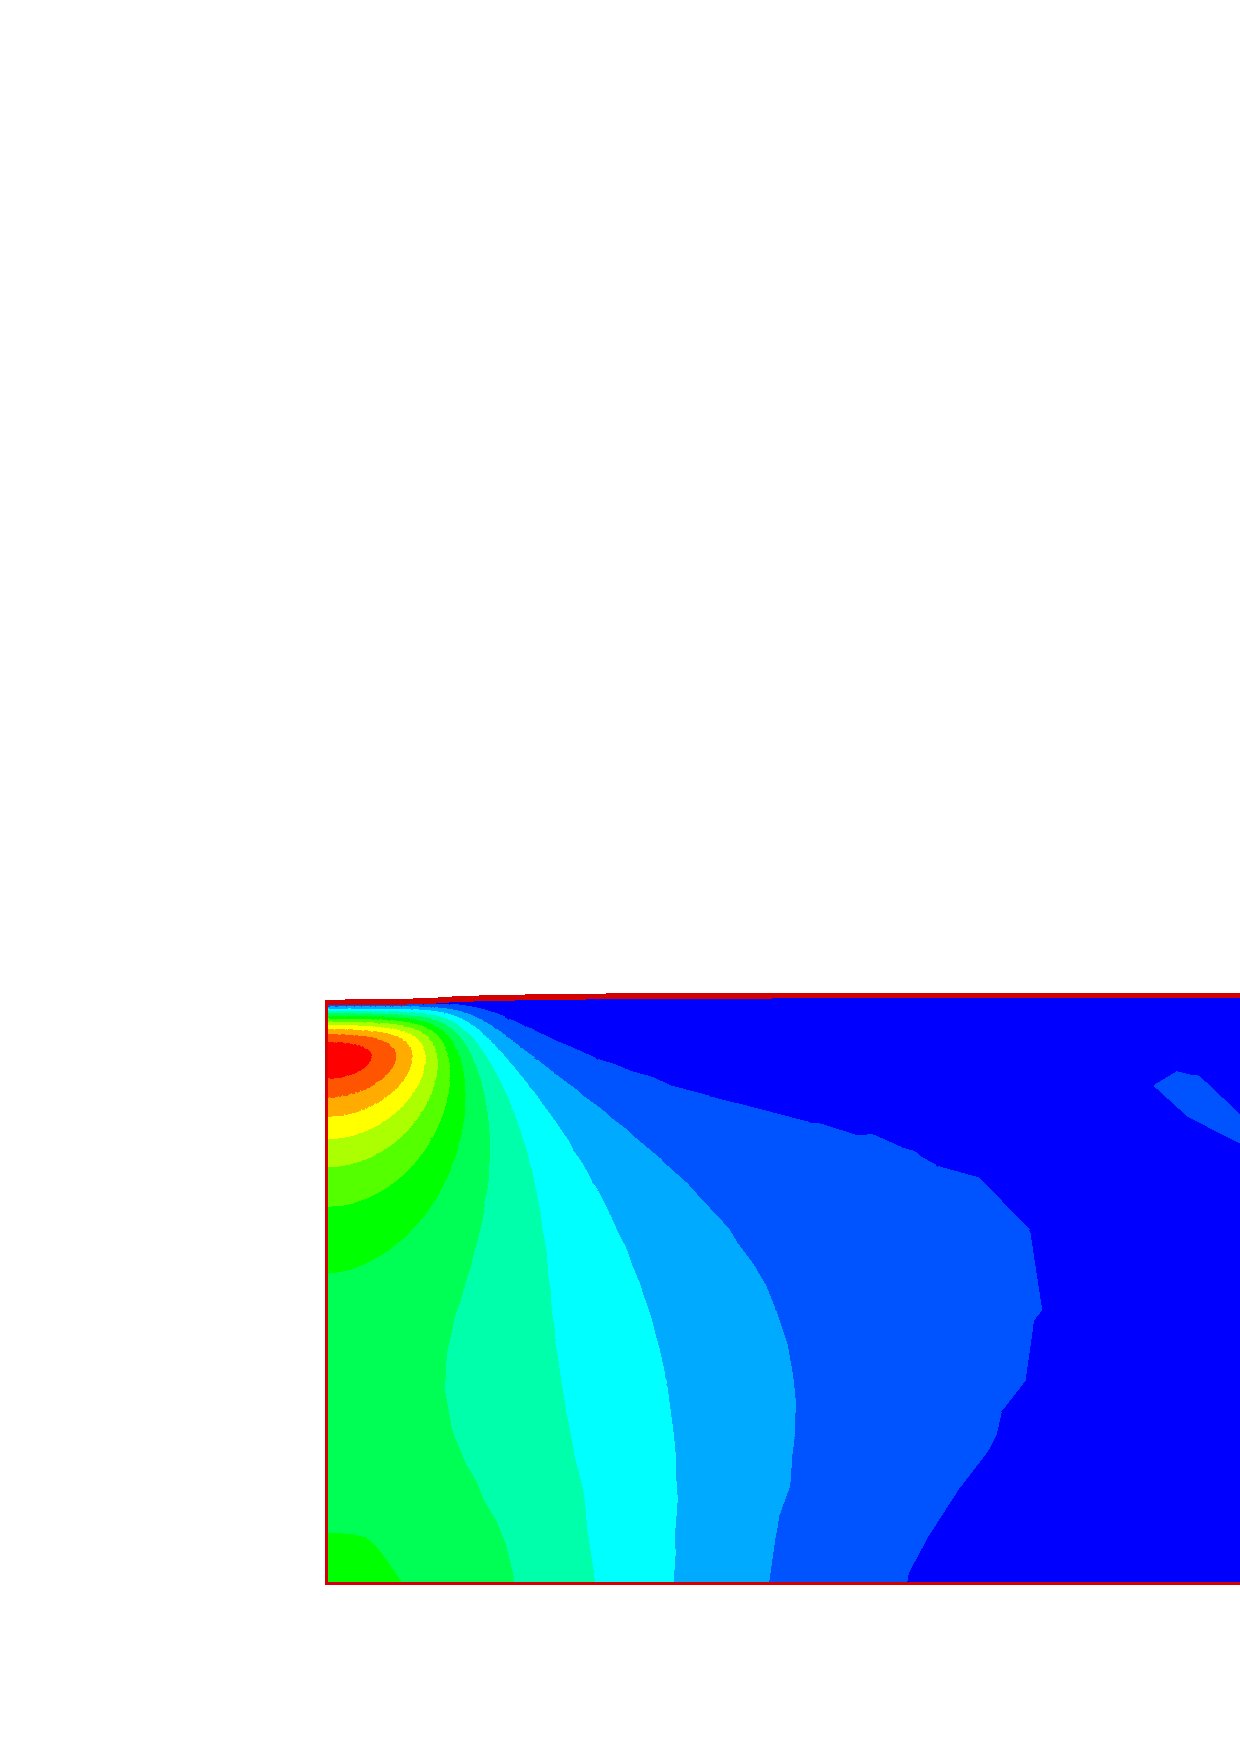
\includegraphics[width=0.49\textwidth]{chapter_14/figures/fig_14_1_6_a}
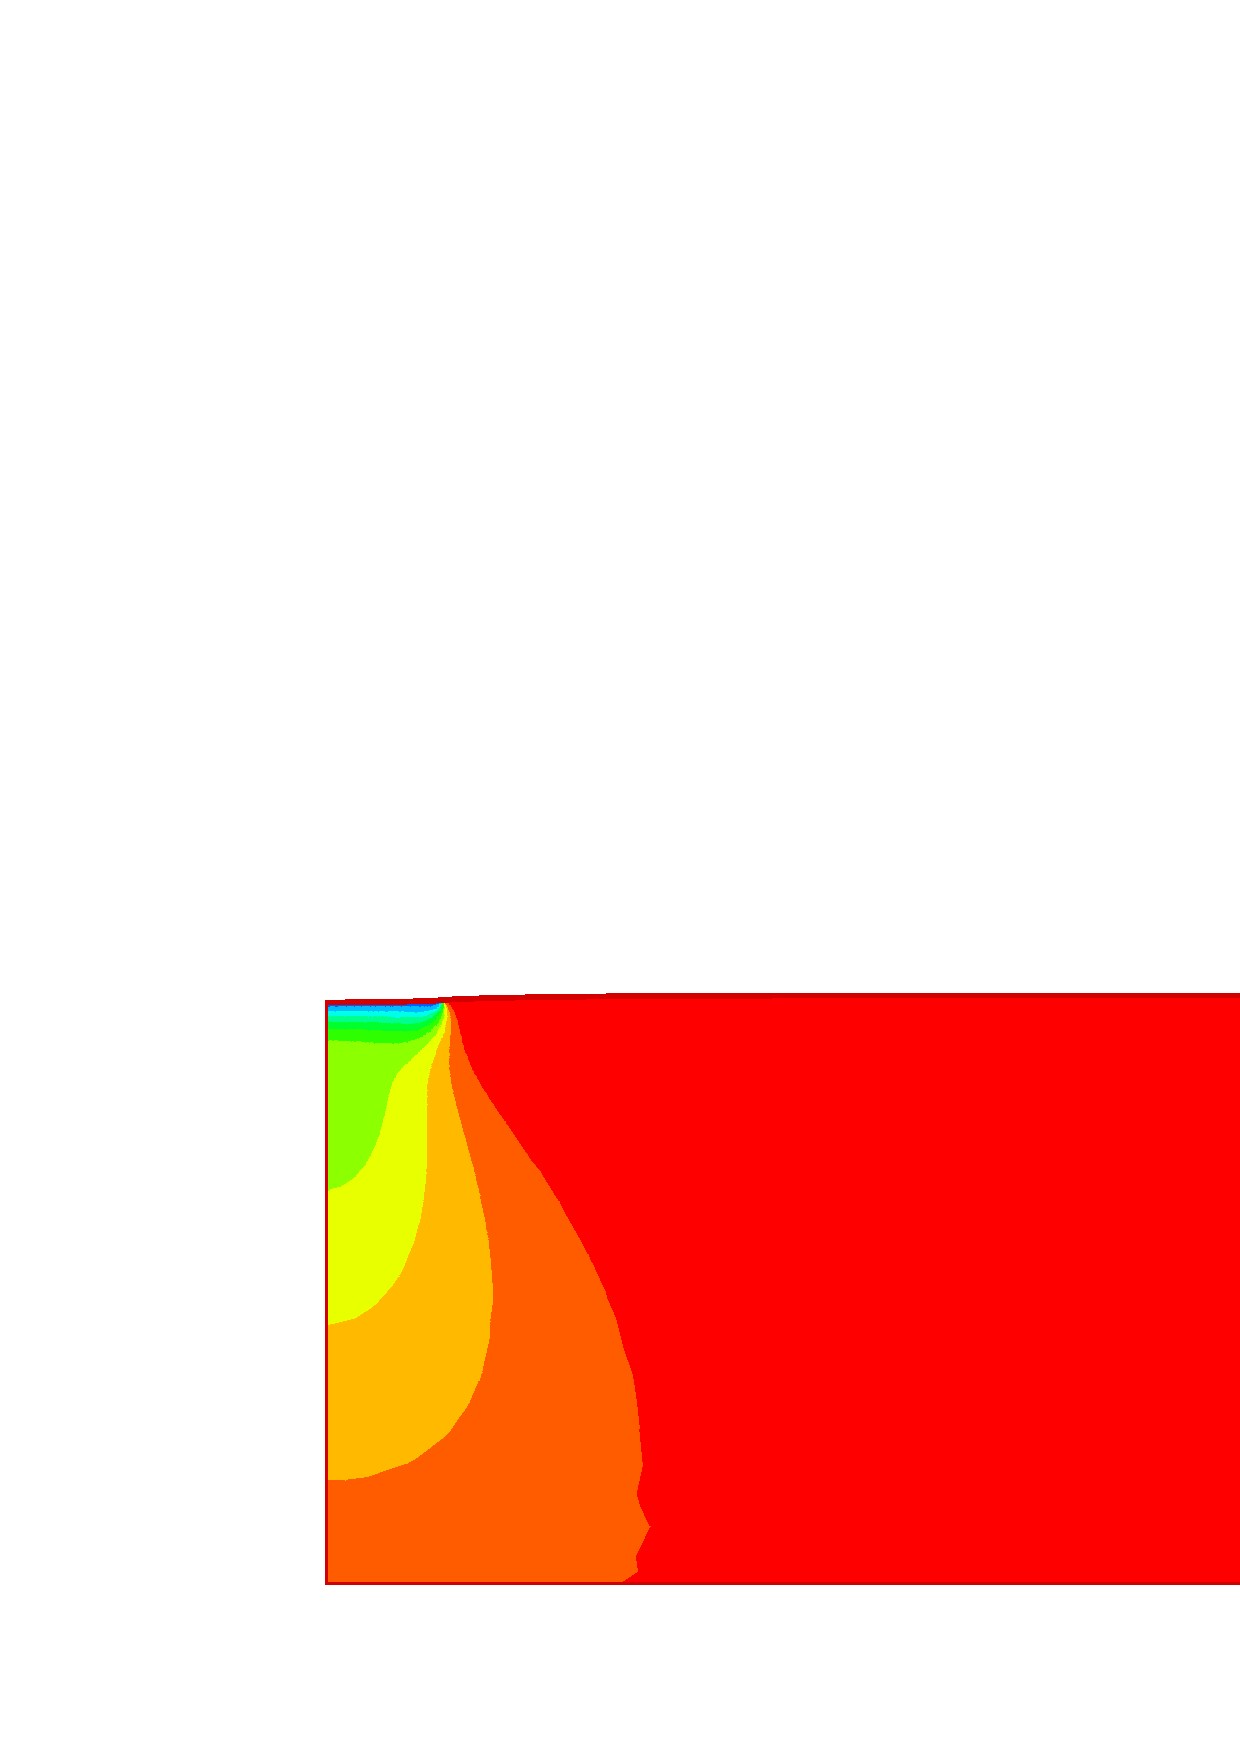
\includegraphics[width=0.49\textwidth]{chapter_14/figures/fig_14_1_6_b}
\end{center}
\vspace{-0.5cm}
\caption{2D contours.}
\label{fig:e10}

\begin{center}
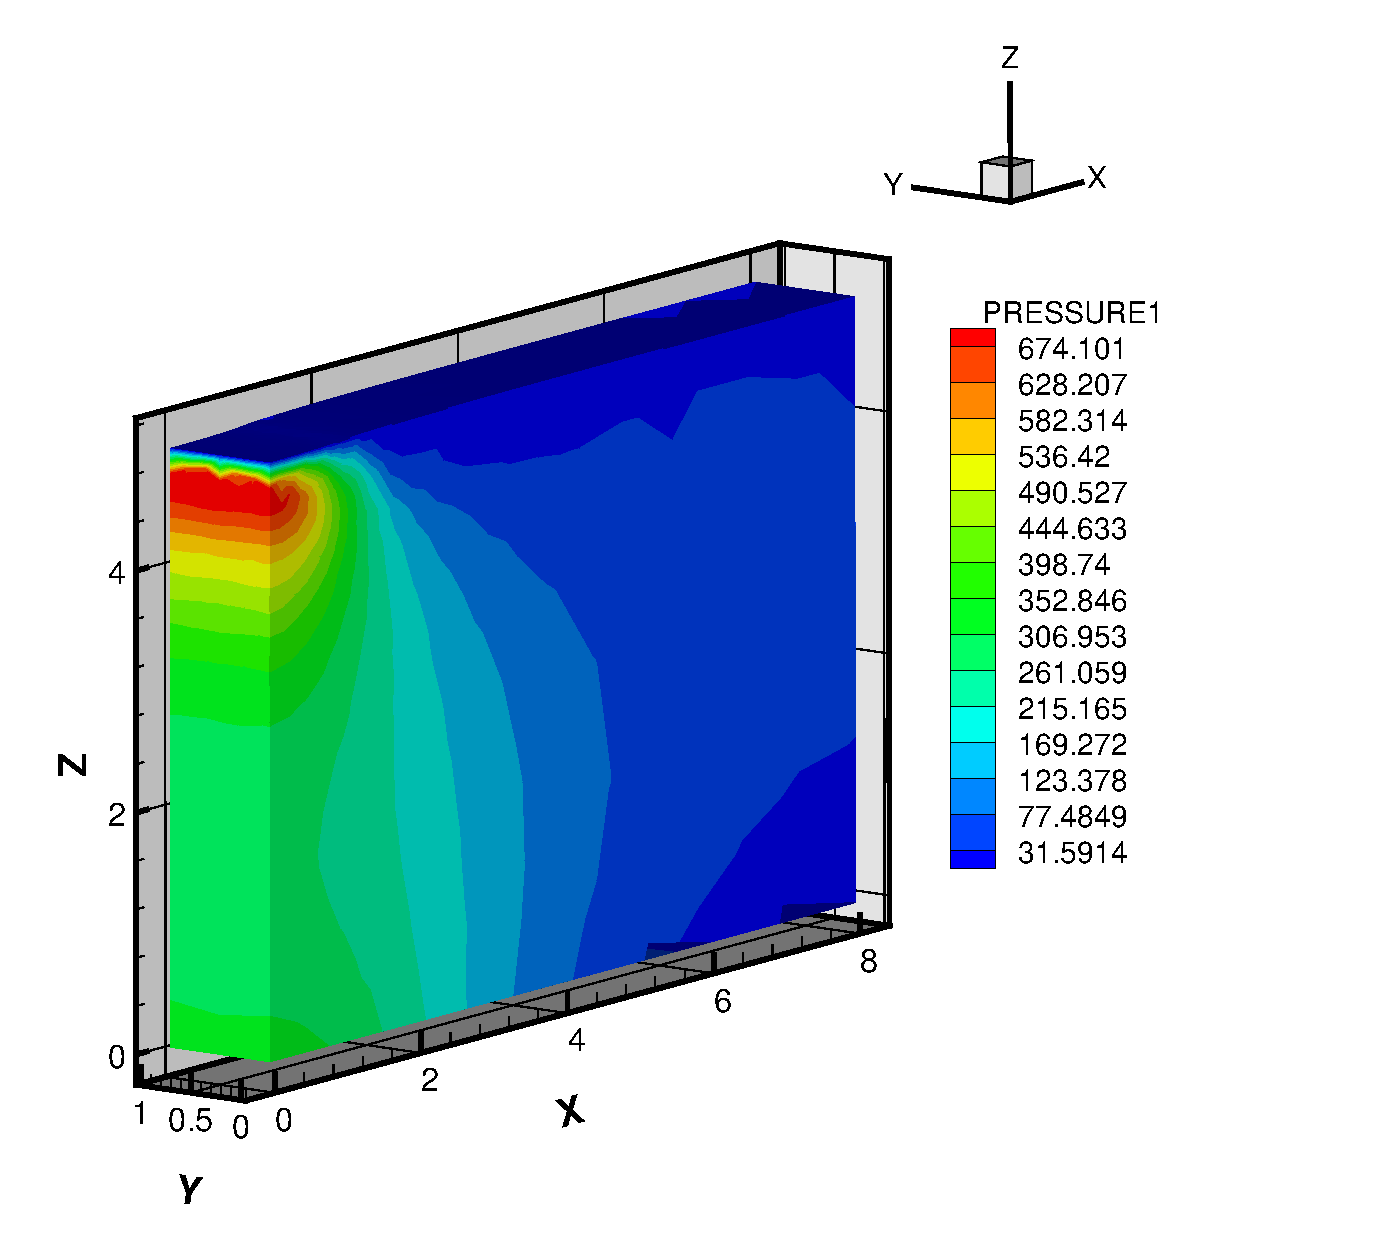
\includegraphics[width=0.49\textwidth]{chapter_14/figures/fig_14_1_7_a}
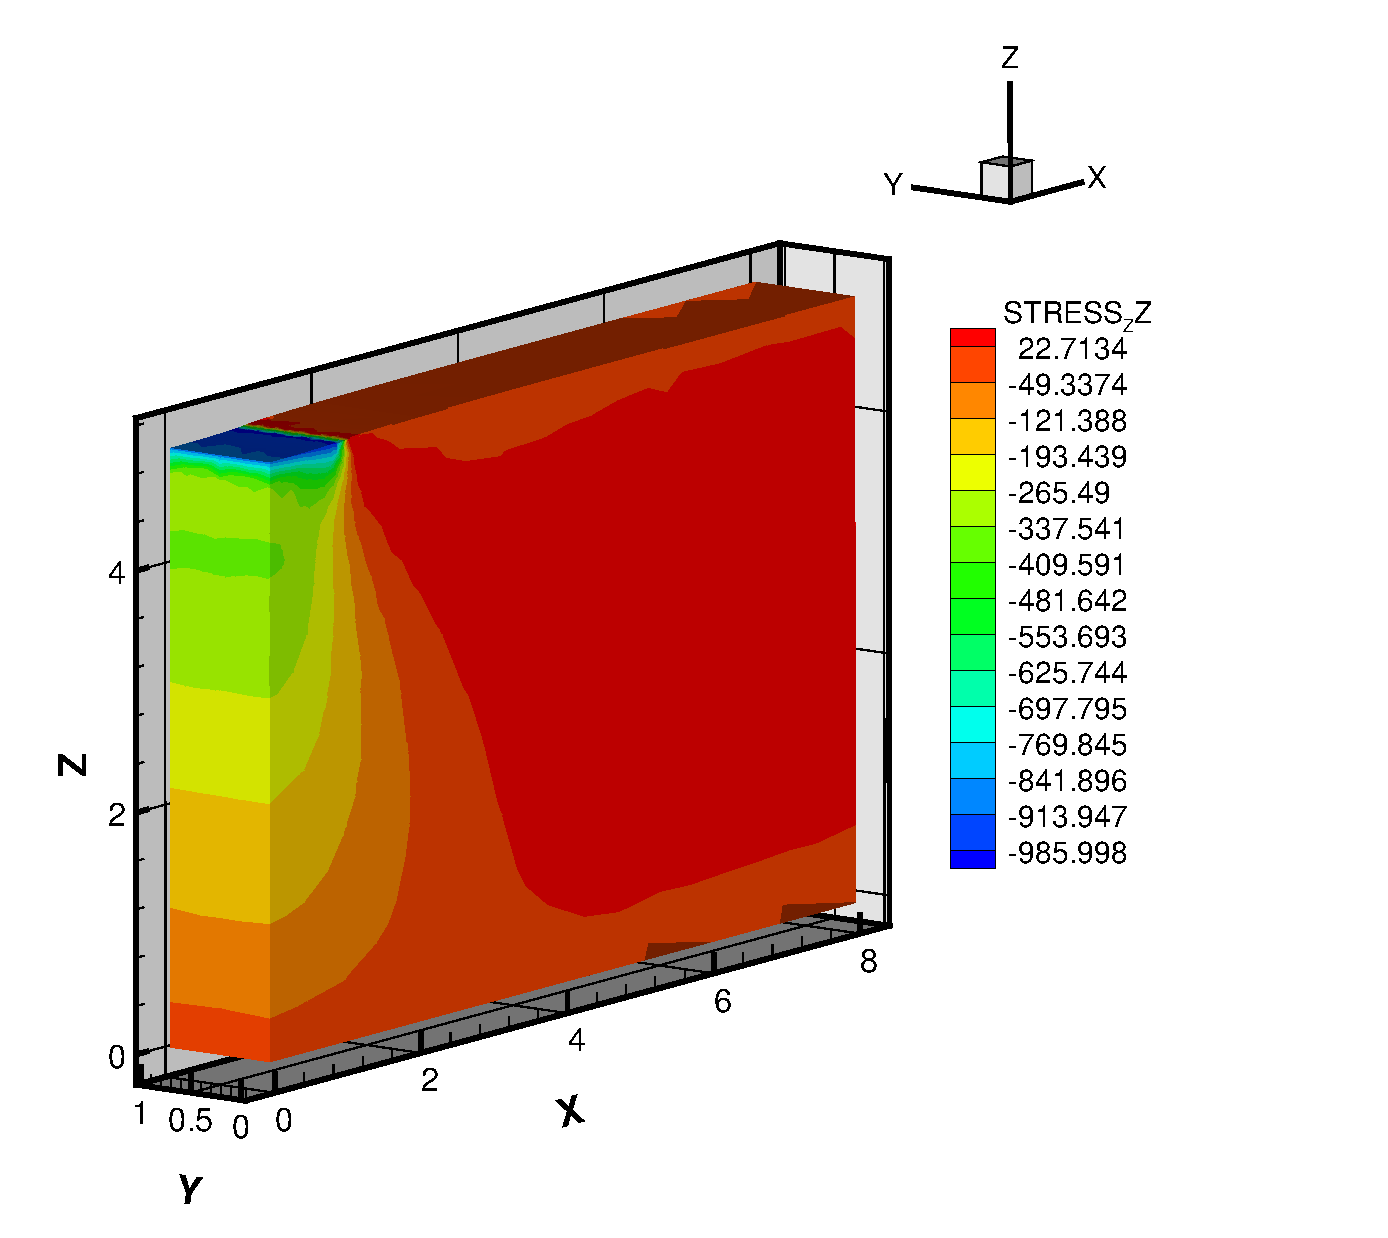
\includegraphics[width=0.49\textwidth]{chapter_14/figures/fig_14_1_7_b}
\end{center}
\vspace{-0.5cm}
\caption{3D contours.}
\label{fig:e12}
\end{figure}
\subsection{Distributed footing: Poroelastic cube (3D) with dynamic consolidation}
Considering the same problem design as the previous section, the mechanical calculation is now extended to allow for time-dependent deformation. In other words, solid displacements are no longer solved to equilibrium, so that solid velocity may be non-zero following solution of the mechanical system.

\subsubsection*{Definition}
All stresses and pressure are zero at the beginning of deformation. Strip
loading ($\sigma_{yy}=\sigma_0$ in $x\in[0,1]$), zero stresses
($\sigma_{yy}=\sigma_{xy}=0$ in $x\in(1,8]$) and zero pressure at
the top; no horizontal flux, no horizontal displacements and zero
shear stresses at left and right hand sides; no vertical flux and no
displacements at bottom (Figure \ref{fig-setting}).

Material parameters are given in Table \ref{tab:mat-dynam}.

\begin{table}[!htb]
\begin{center}
\begin{tabular}{lll}
\hline{\smallskip}
Property & Value & Unit \\
\hline
Young's modulus & $3\times 10^{4}$  & $N/m^{2}$ \\
Poisson's ratio & $0.2, 0.4$       & $-$ \\
Permeability    & $10^{-10}$        & $m^2$ \\
Fluid viscosity & $10^{-3}$         & $Pa\,s$ \\
\hline
\end{tabular}
\end{center}
\caption{Material properties of dynamic consolidation problem.}
\label{tab:mat-dynam}
\end{table}

\subsubsection*{Results}
Time duration is ten time steps. The following figures, Fig. \ref{fig_dynHM1}--\ref{fig_dynHM4} show the distribution of state variables within the domain after 10 time steps. Such distribution is similar to the static case illustrated in Fig. \ref{fig:e10}.
 
\begin{figure}[!htb]
\begin{center}
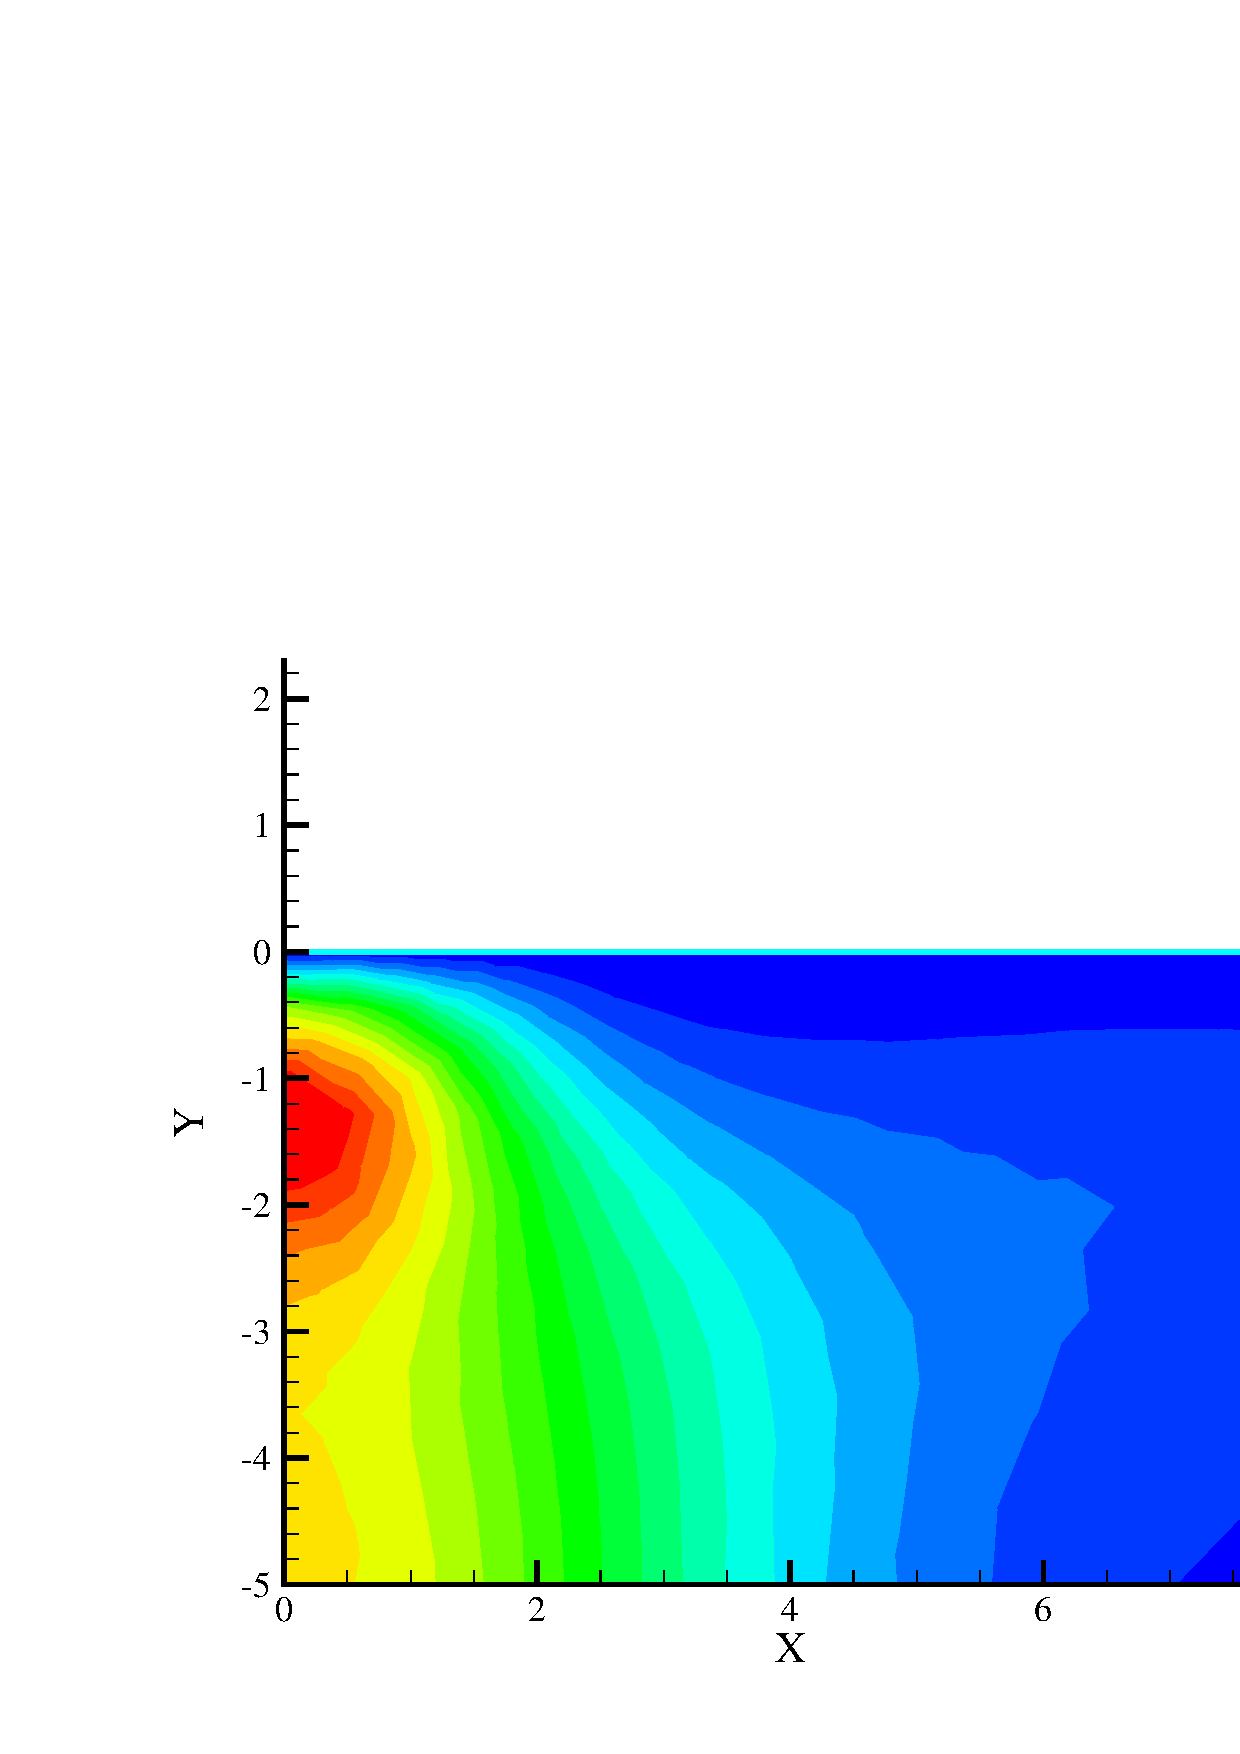
\includegraphics[width=0.49\textwidth]{chapter_14/figures/fig_14_1_8_a}
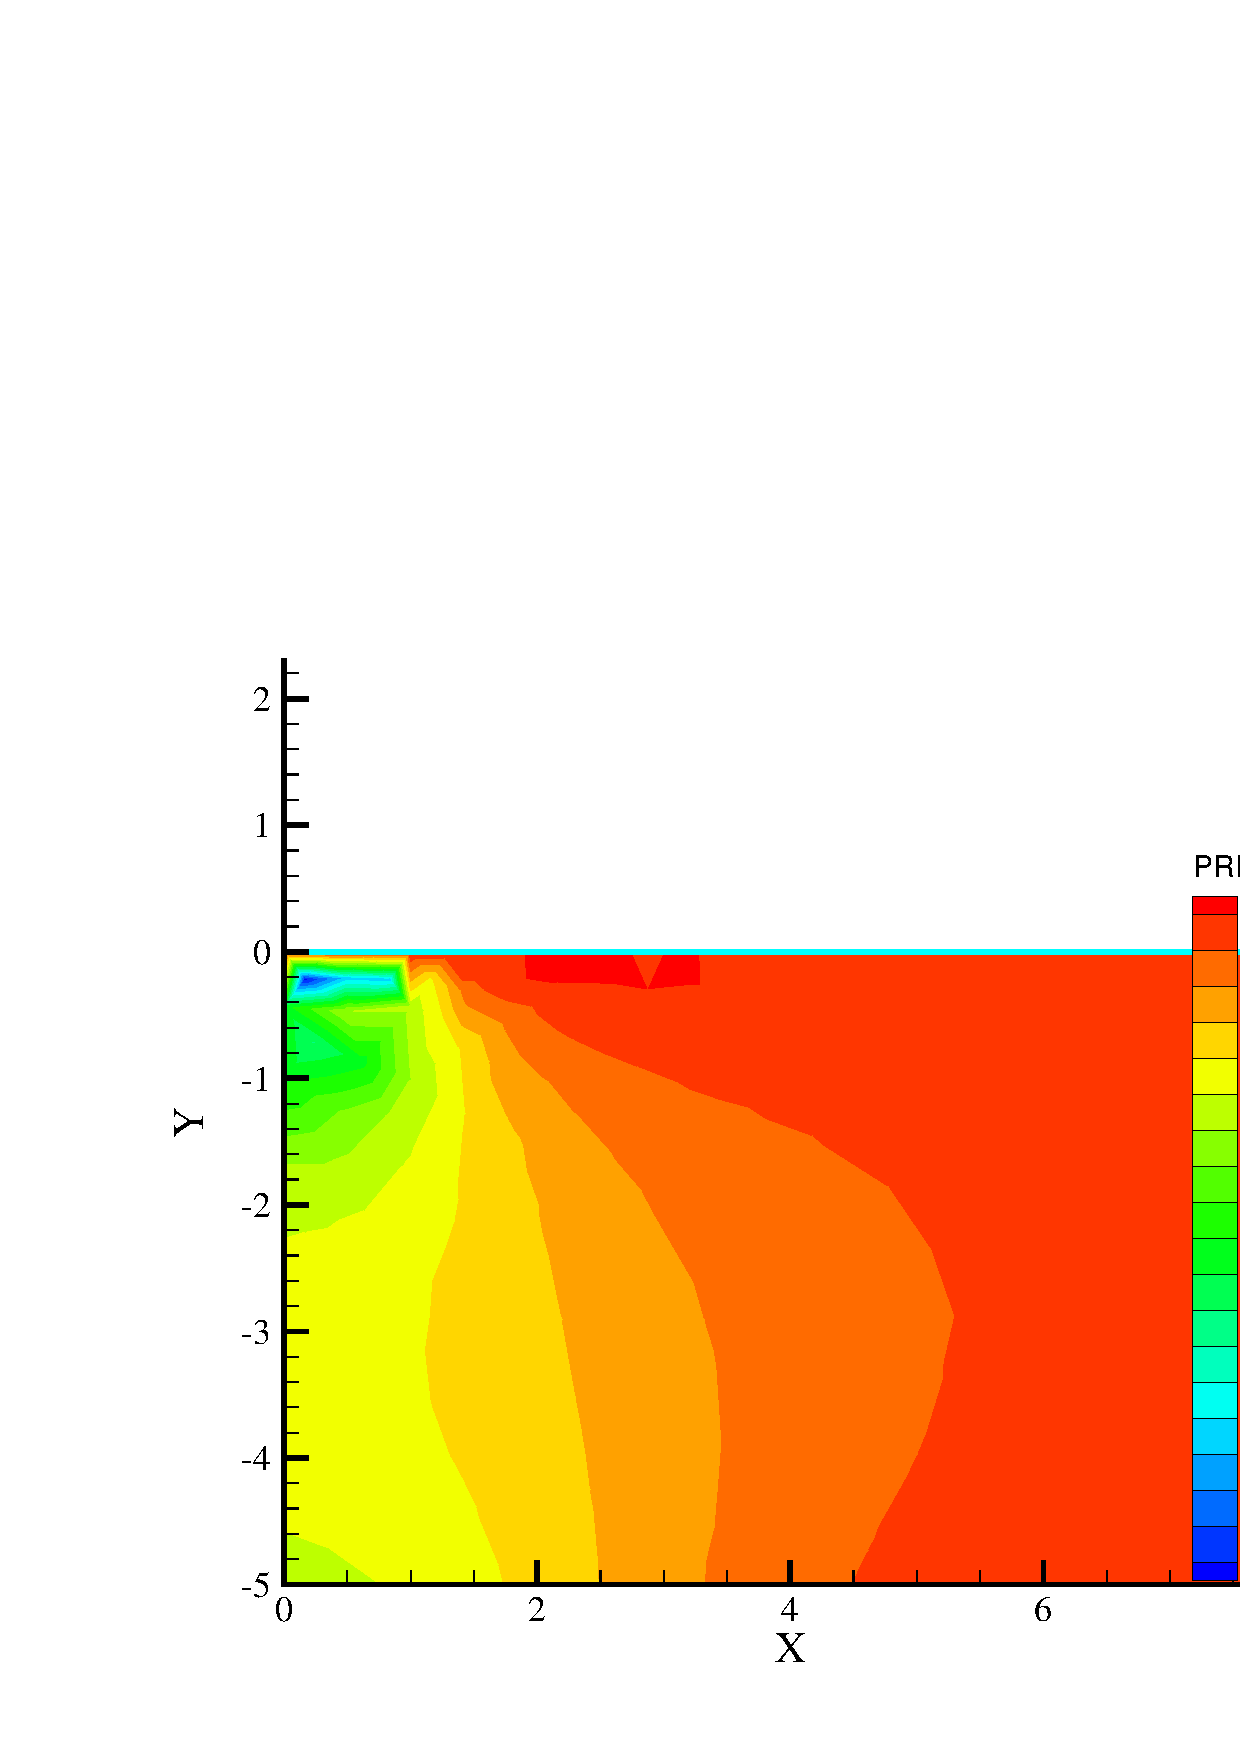
\includegraphics[width=0.49\textwidth]{chapter_14/figures/fig_14_1_8_b}
\end{center}
\caption{Fluid pressures $p$ and rate of fluid pressure $\dot p$ }
\label{fig_dynHM1}
\end{figure}

\begin{figure}[!htb]
\begin{center}
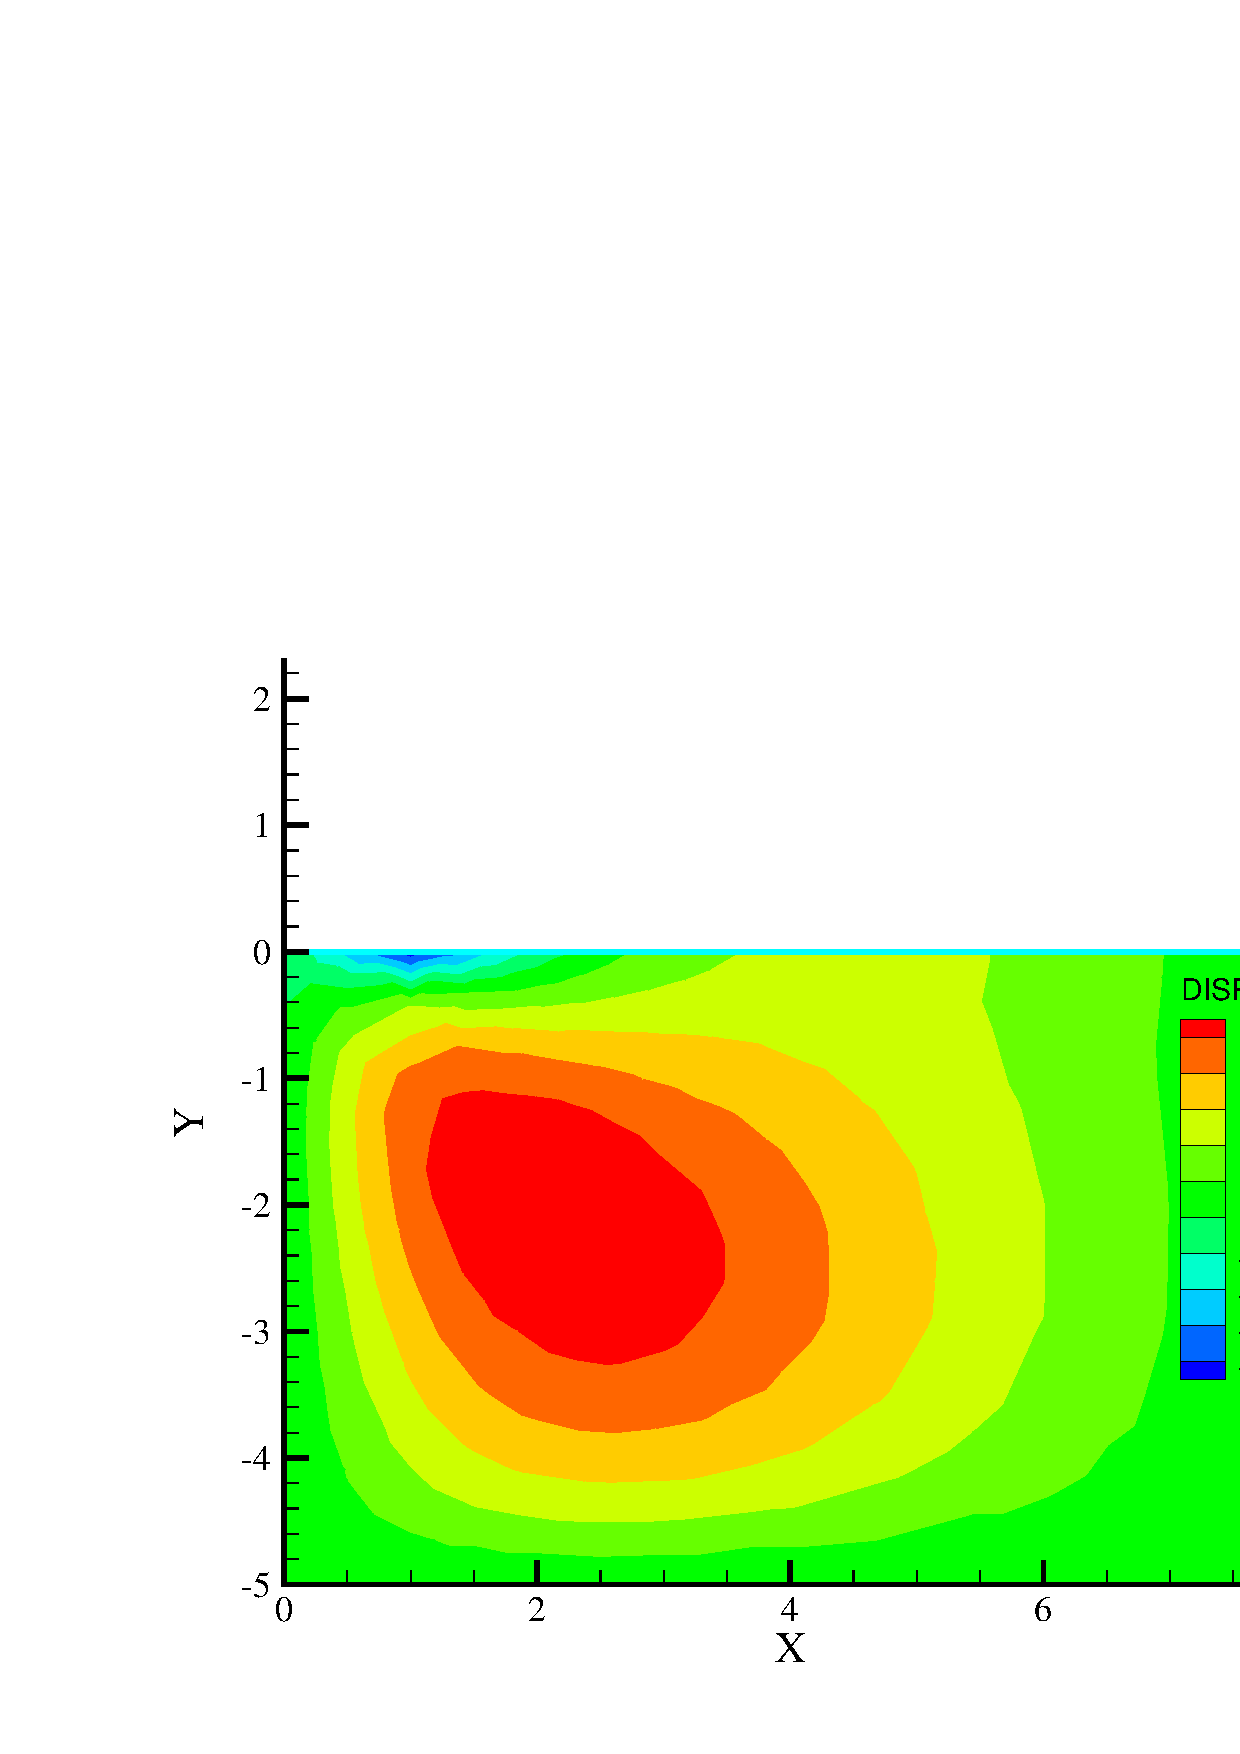
\includegraphics[width=0.32\textwidth]{chapter_14/figures/fig_14_1_9_a}
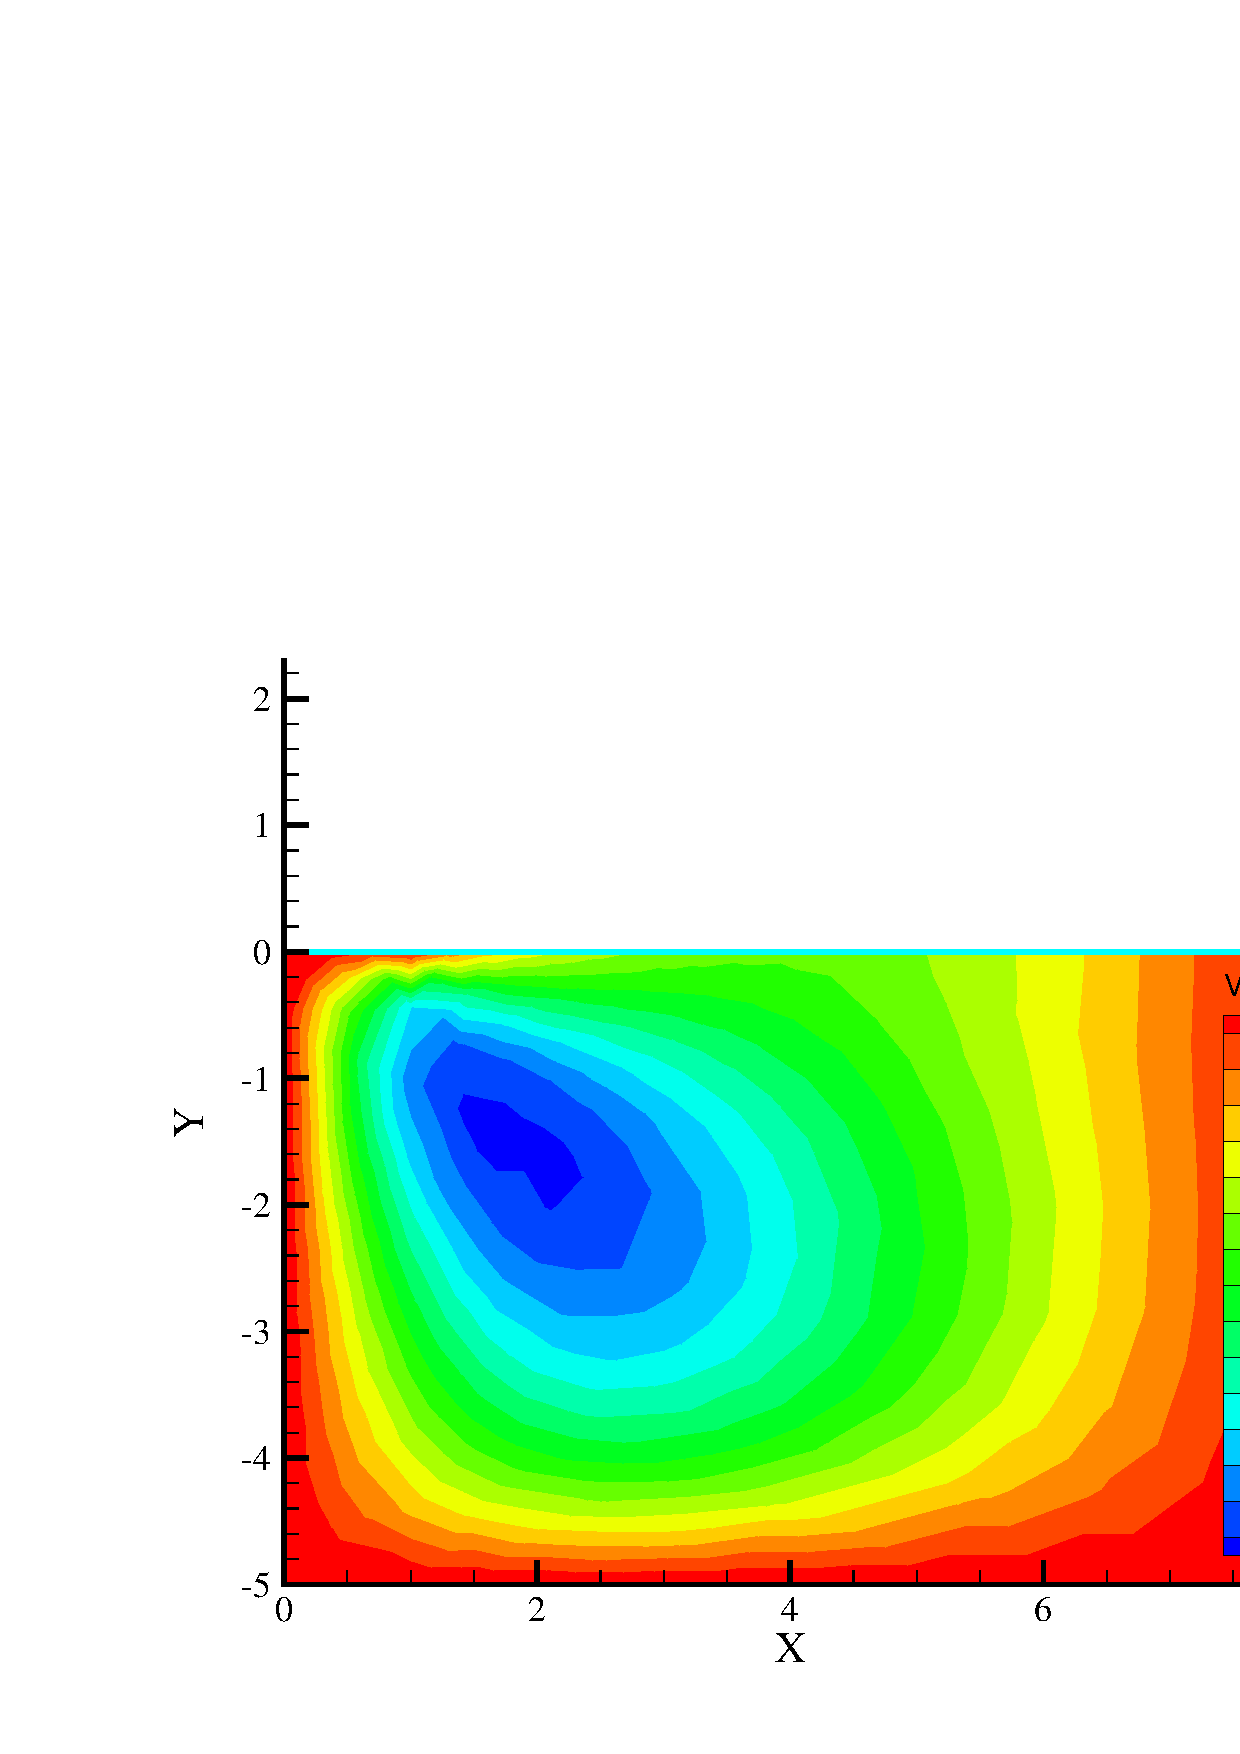
\includegraphics[width=0.32\textwidth]{chapter_14/figures/fig_14_1_9_b}
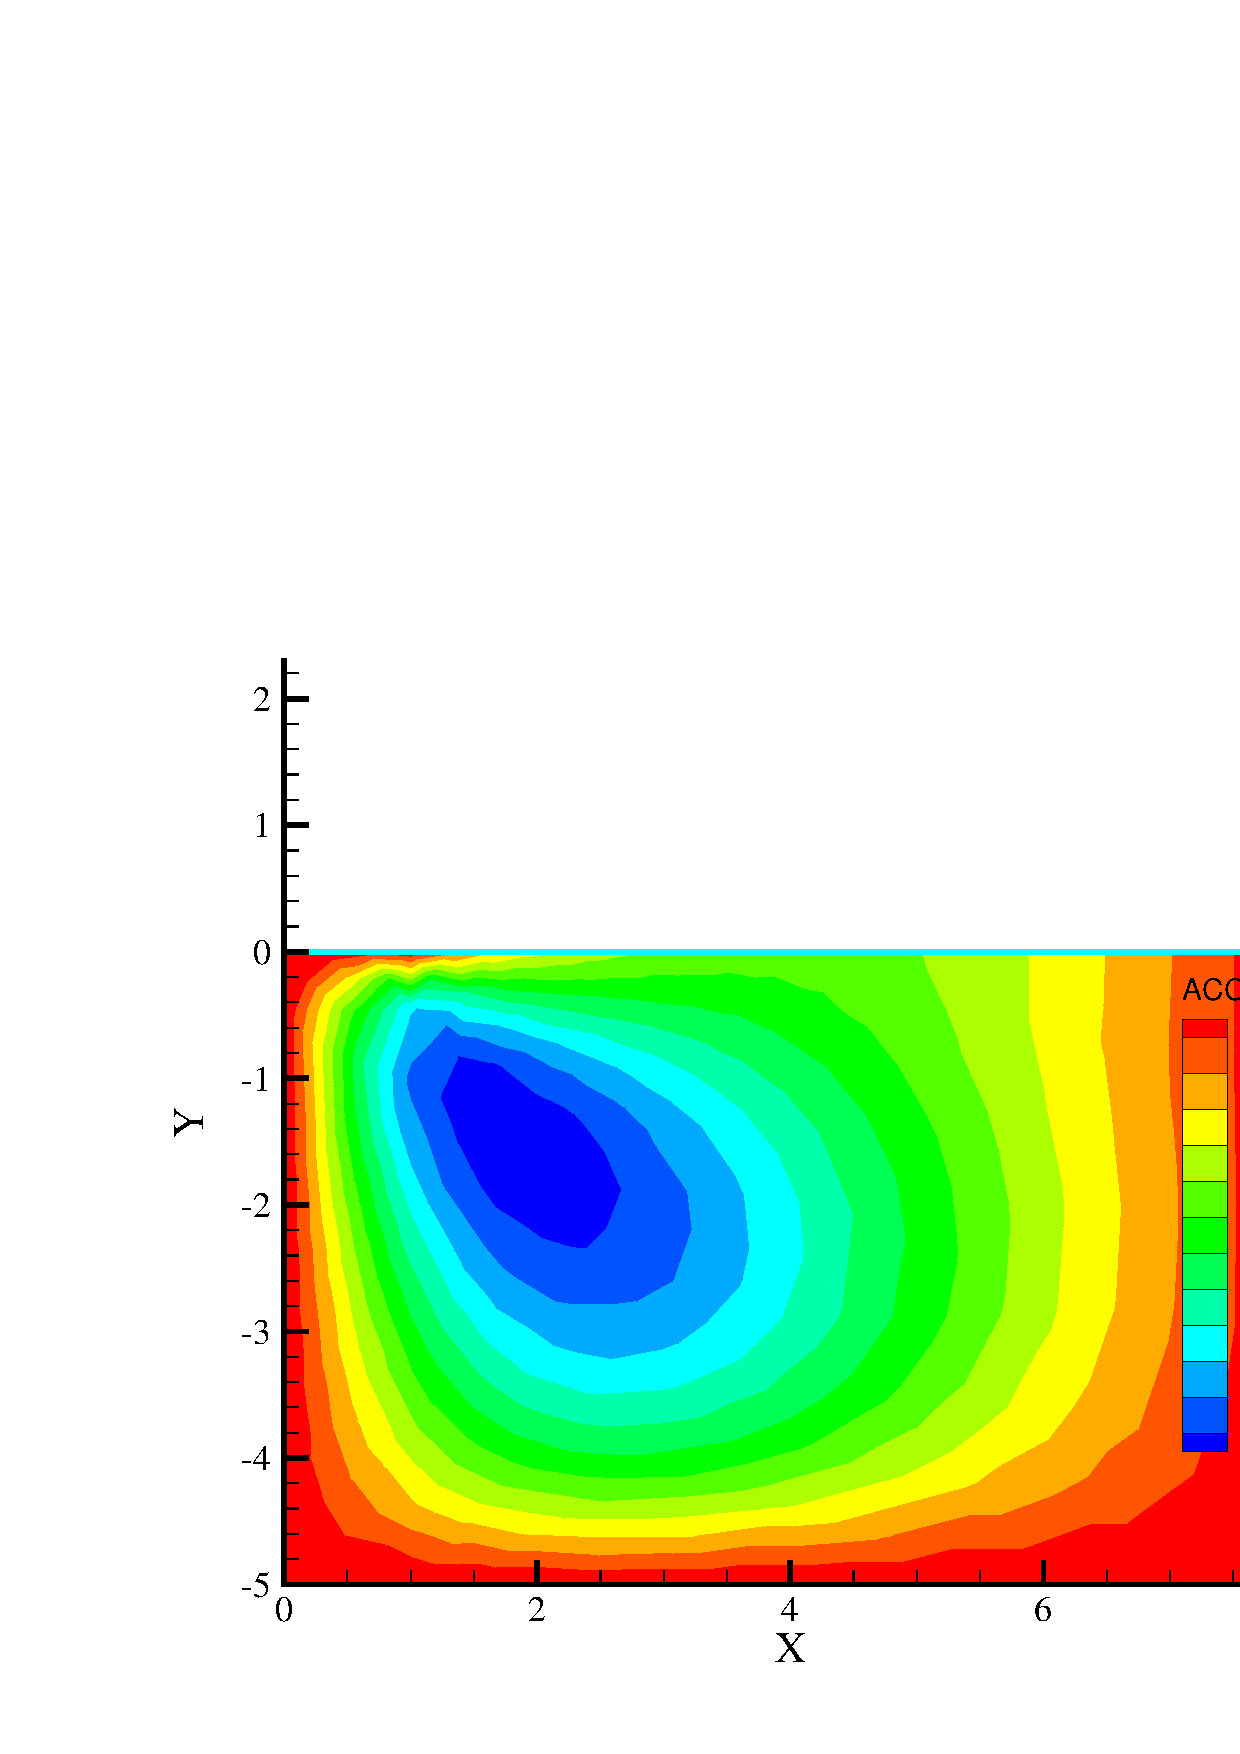
\includegraphics[width=0.32\textwidth]{chapter_14/figures/fig_14_1_9_c}
\end{center}
\caption{Displacement, its rate and acceleration: horizontal component}
\label{fig_dynHM2}
%\end{figure}
%\begin{figure}[!htb]
\begin{center}
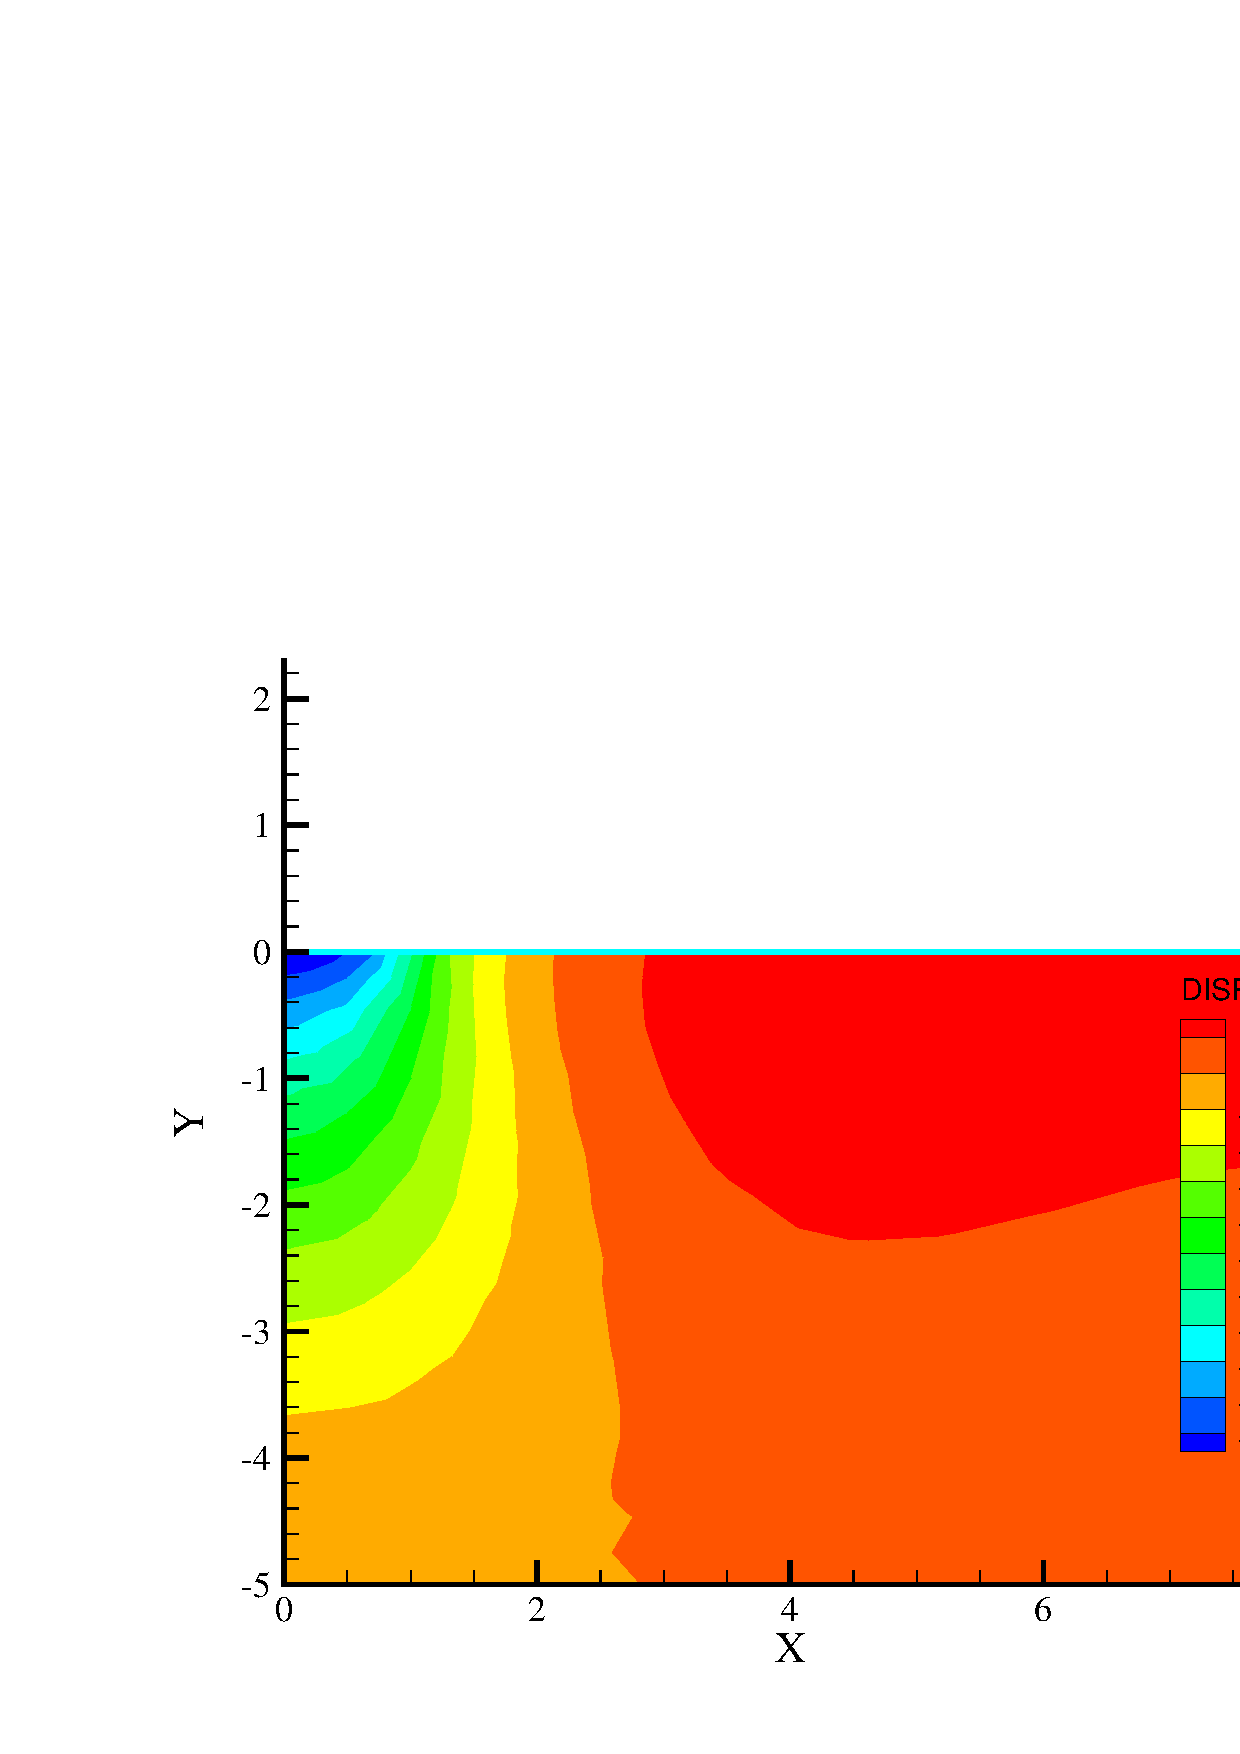
\includegraphics[width=0.32\textwidth]{chapter_14/figures/fig_14_1_10_a}
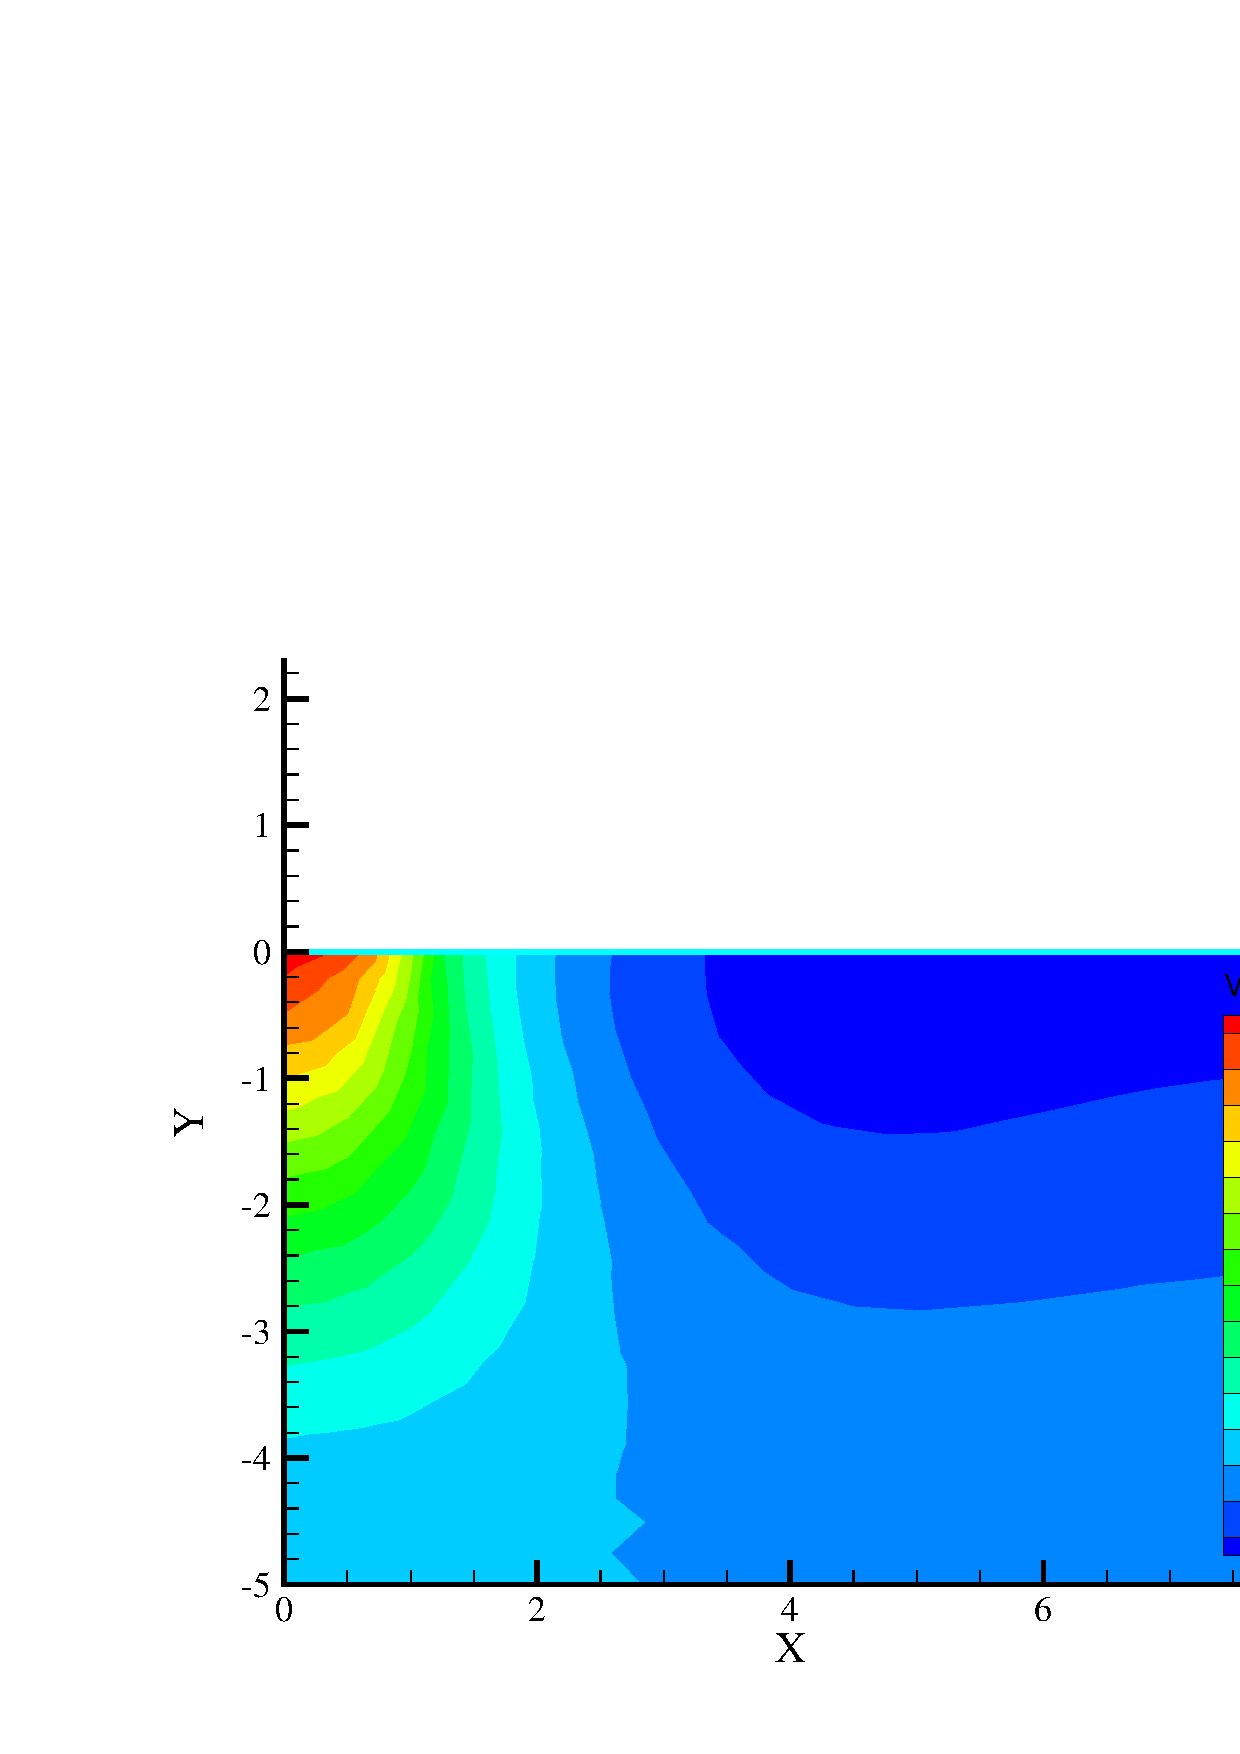
\includegraphics[width=0.32\textwidth]{chapter_14/figures/fig_14_1_10_b}
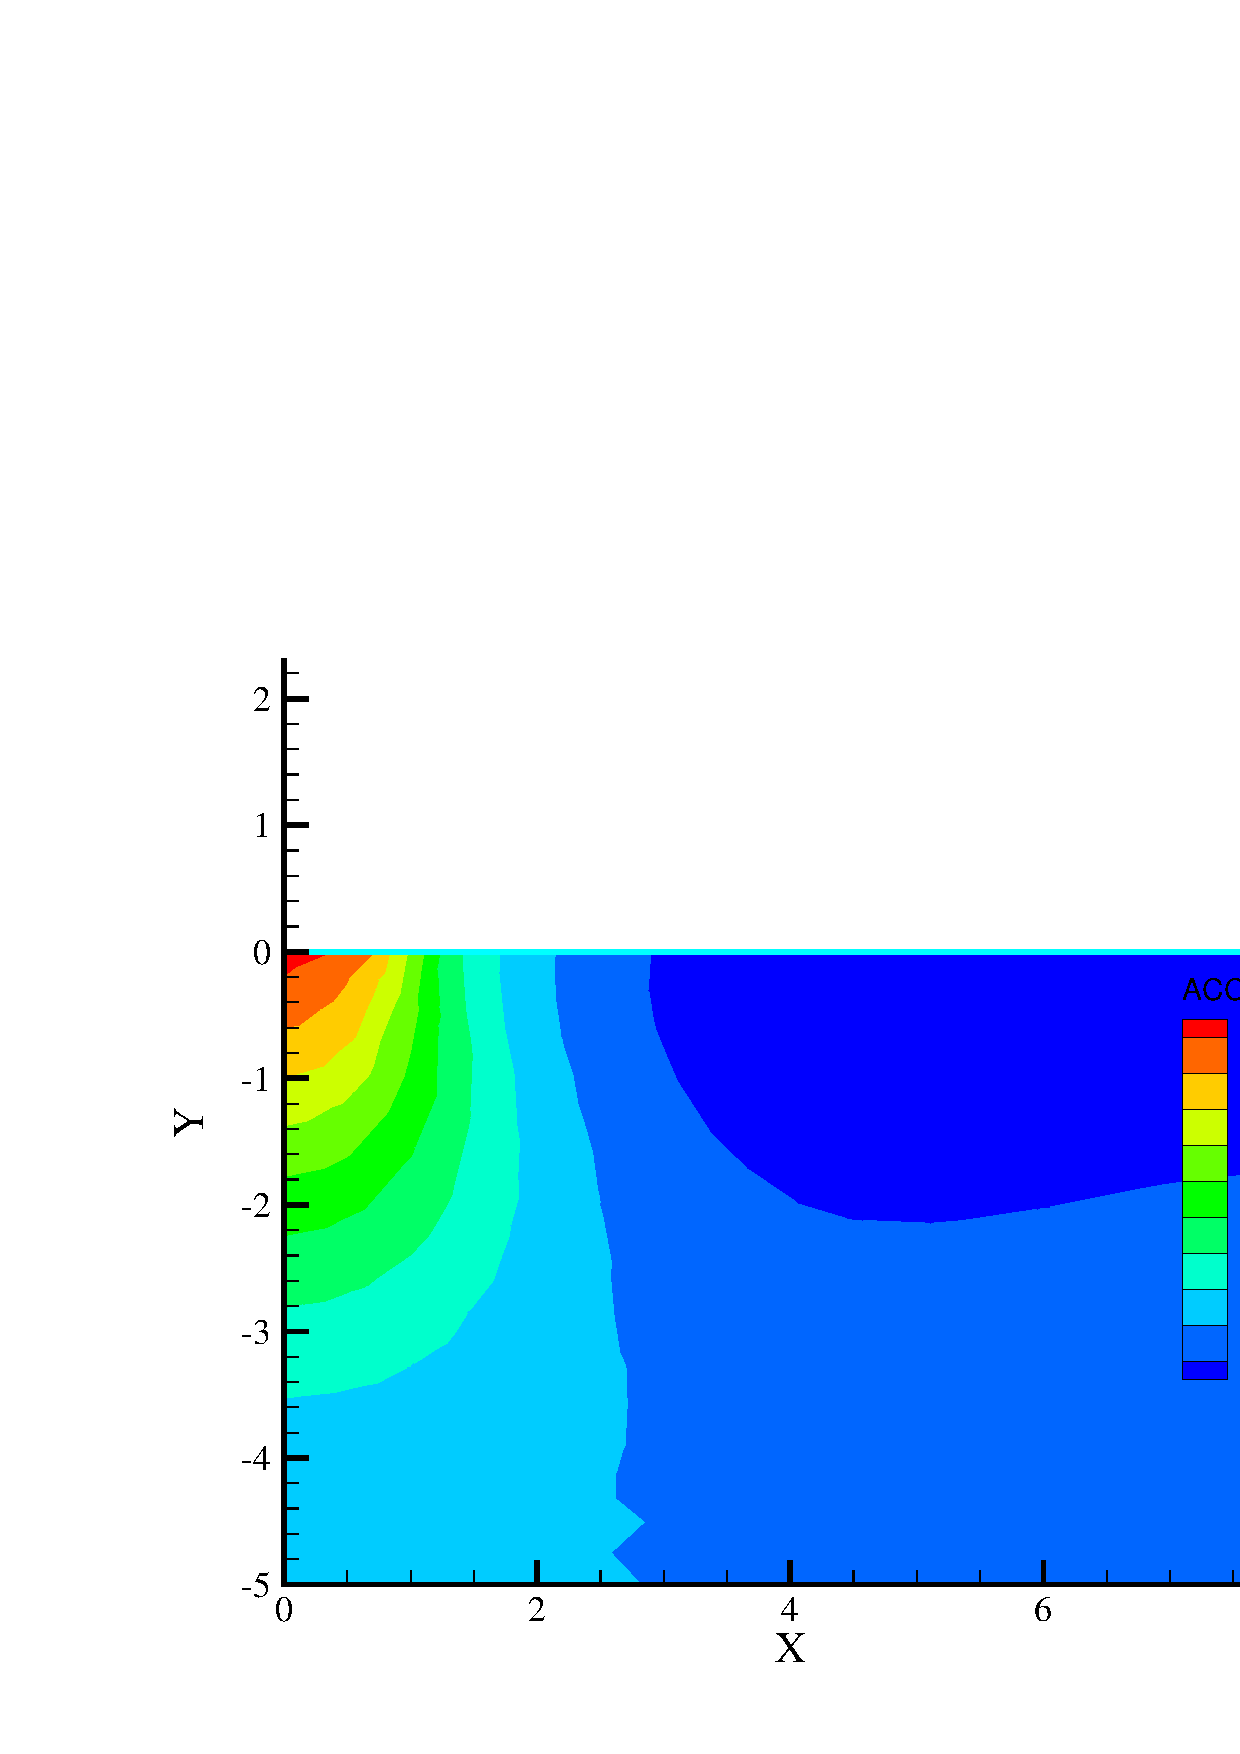
\includegraphics[width=0.32\textwidth]{chapter_14/figures/fig_14_1_10_c}
\end{center}
\caption{Displacement, its rate and acceleration: vertical component}
\label{fig_dynHM3}
\end{figure}
\begin{figure}[!htb]
\begin{center}
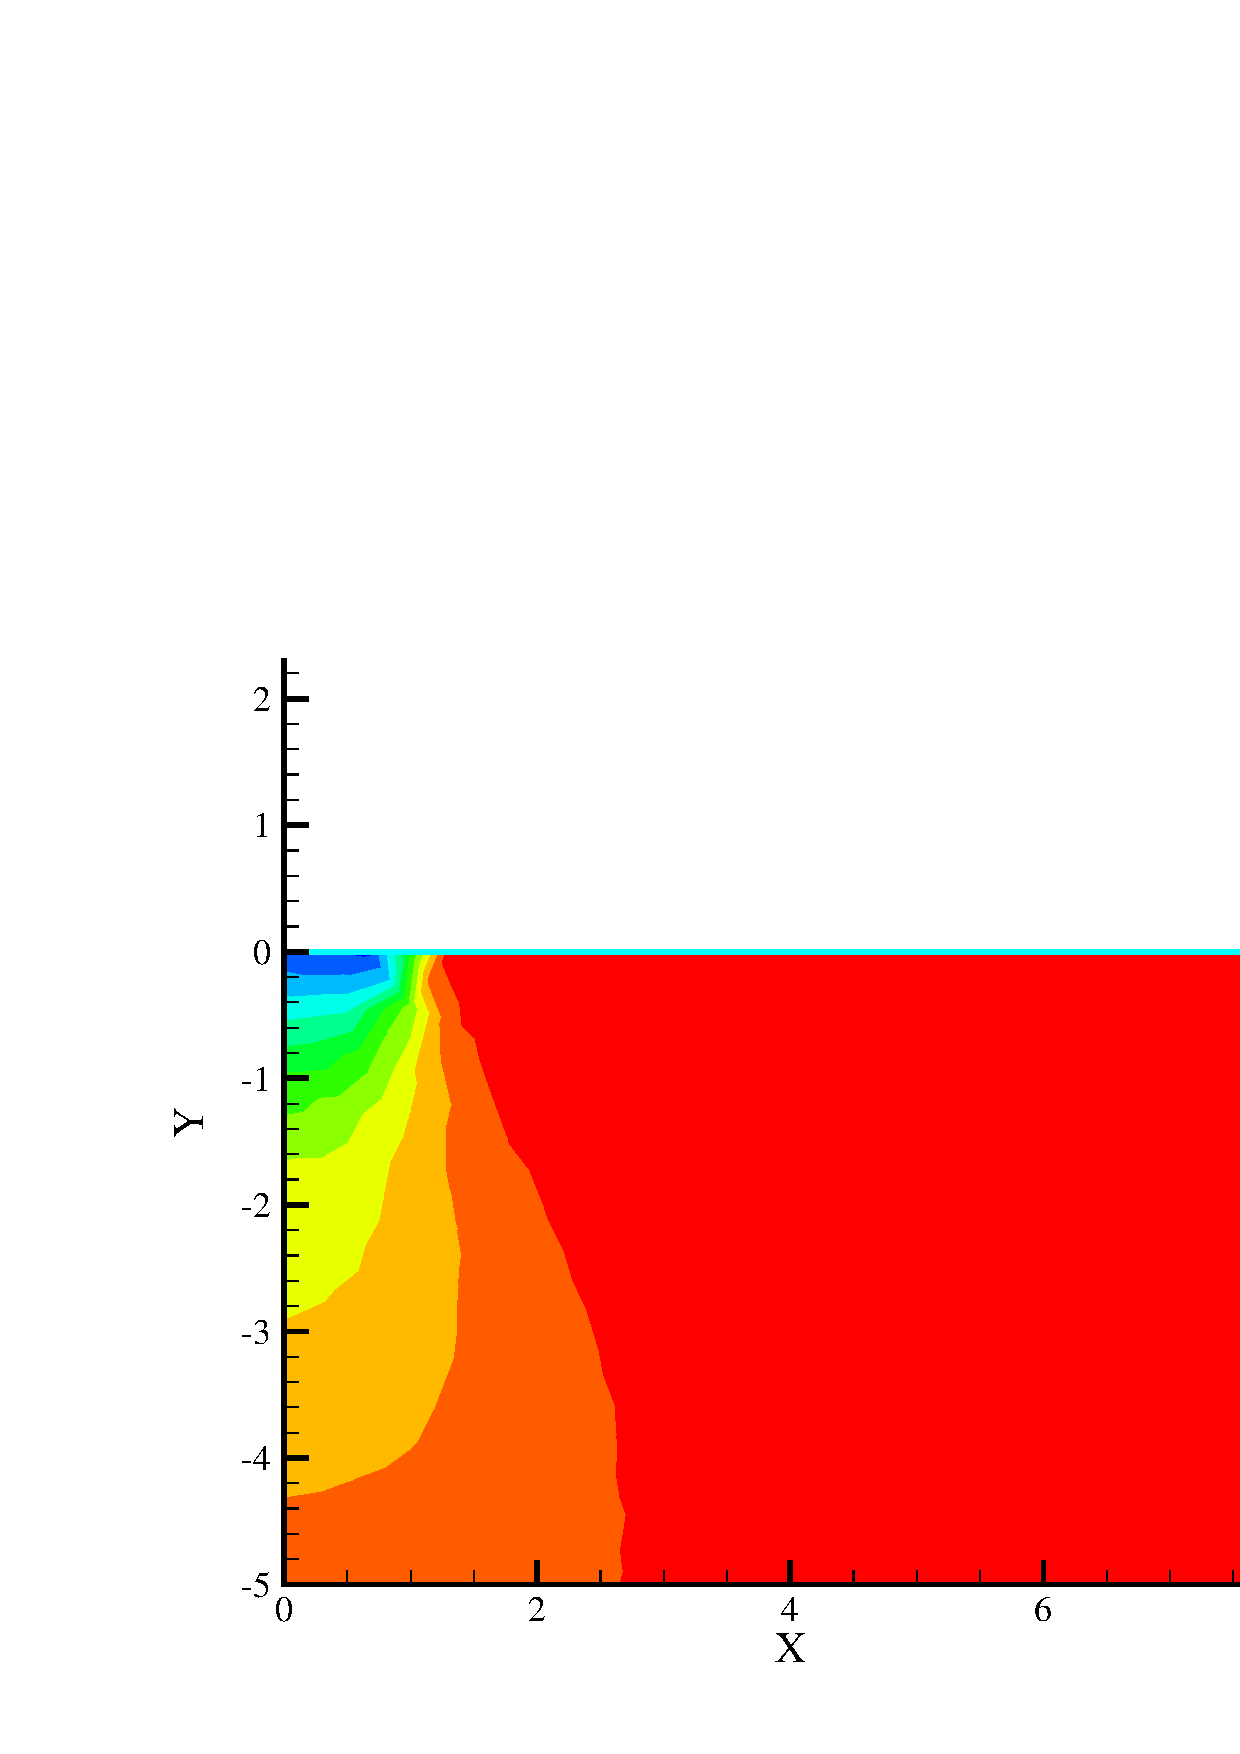
\includegraphics[width=0.5\textwidth]{chapter_14/figures/fig_14_1_11}
\end{center}
\caption{Vertical stress.}
\label{fig_dynHM4}
\end{figure}














%\section{Unsaturated}
\section{Unsaturated (Richards) consolidation}

\subsubsection*{Fluid mass and momentum balance}
The general fluid mass balance equation for a multi-phase fluid system is simply an extension of Eq. \ref{eqch14:genmass},

\begin{equation}
\frac{\partial }{\partial t}\left( \phi {{S}_{\alpha }}\rho  \right)+\frac{\partial }{\partial {{x}_{i}}}\left( \phi {{S}_{\alpha }}\rho {{v}_{i}} \right)=Q
\end{equation}

where $S_\alpha$ is saturation of fluid $\alpha $ and $Q$ is the source term. We are interested in a Richards type model for the evolution of fluid pressure under the assumption that the gas phase is immobile, i.e. $v_{gi}=0$. Assuming incompressible grains, $\alpha =0$, and expanding terms as in the single phase case, we obtain the following Richards equation for an unsaturated deformable porous medium,

\begin{eqnarray}
\left( {{S}_{w}}\frac{\phi }{{{K}_{w}}}\frac{d{{p}_{w}}}{dt}-\phi {{\rho }_{w}}\frac{d{{S}_{nw}}}{d{{p}_{c}}} \right)\frac{d{{p}_{w}}}{dt}+\nabla \cdot \left\{ \frac{\mathbf{k}k_{w}^{r}}{{{\mu }_{w}}}\left( -\nabla {{p}_{w}}+{{\rho }_{w}}\mathbf{g} \right) \right\}+\nonumber\\
{{\text{S}}_{w}}{{\rho }_{w}}\nabla \cdot \frac{d\mathbf{u}}{dt}=Q.
\label{eqn:uc2}
\end{eqnarray}

A constitutive equation, the water content function obtained by experiments, characterizes the relationship between $p_c$ and $\sat _w$, and therefore the derivative $dS_w/dp_c$.

\subsubsection*{Solid momentum balance}
The deformation process is described in the same manner as for the single phase case, but now fluid pressure acting on the grains is also dependent on the liquid saturation,

\begin{eqnarray}
\nabla\cdot
(\sigma - S_w p_w \bf I) + \rho g = 0
\label{eqn:mb_us}
\end{eqnarray}

\subsubsection*{FEM solution scheme}
The standard Galerkin finite element approach is applied for the numerical solution of the PDEs (\ref{eqn:uc2}) and (\ref{eqn:mb_us}) resulting into the following system of algebraic equations, here solved as a monolithic system,

\begin{eqnarray}
\left[
\begin{array}{cc}
\mathbf{C}_{pp} & \mathbf{C}_{pu}
\\
\mathbf{0} & \mathbf{0}
\end{array}
\right]
\frac{d}{dt}
\left\{
\begin{array}{l}
\mathbf{p_w}
\\
\mathbf{u}
\end{array}
\right\}
+
\left[
\begin{array}{ll}
\mathbf{K}_{pp} & \mathbf{0}
\\
\mathbf{K}_{up} & \mathbf{K}_{uu}
\end{array}
\right]
%
\left\{
\begin{array}{l}
\mathbf{p_w}
\\
\mathbf{u}
\end{array}
\right\}
=
\left\{
\begin{array}{l}
\mathbf{r}_p
\\
\mathbf{r}_u
\end{array}
\right\}
\nonumber
\\
\end{eqnarray}
%-------------------------------------------------------------------------
%-------------------------------------------------------------------------

\subsection{Heat Pipe problem}
\subsubsection*{Background}
When an unsaturated porous medium subjected to a constant heat flux and the temperature is sufficiently high, water is heated and vaporizes. Vapor flows under its pressure gradient towards the cooler end where it condenses. Vaporization and condensation produce a liquid saturation gradient, creating a capillary pressure gradient inside the porous medium. Condensate flows towards the hot end under the influence of a capillary pressure gradient. This is a heat pipe in an unsaturated porous medium

Udell and Fitch derived the pressure gradient of each phase in two-phase flow with heat transfer. The generalized form of the Darcy's law is used to calculate velocity fields. 
\begin{equation}
\frac{d p^g}{d x} = \frac{\eta q \nu^g}{\mathbf k k_{\mathrm {rg}} H_{\mathrm {vap}}}
\label{eq:HP1}
\end{equation}
\begin{equation}
\frac{d p^l}{d x} =- \frac{\eta q \nu^l}{\mathbf k k_{\mathrm {rl}} H_{\mathrm {vap}}}
\label{eq:HP2}
\end{equation}
where, $\eta$ is the ratio of heat transport caused by convection to the total heat-flux $q$ (see Helming [1997]). $p$ is phase pressure; $\nu^\gamma=\frac{\mu\gamma}{\rho^\gamma}$; $x$ is space coordinate in the x-direction; $\mathbf k$ is intrinsic permeability; $k_{r\gamma}$ is relative permeability and $H_{\mathrm {vap}}$ is latent heat of water. $\gamma$ is the phase superscript and $g, l$ stand for gas and liquid phase, respectively. Gas pressure is the sum of two partial pressure, i.e. $p^g=p^g_a+p^g_w$.

The density of the gas phase is the sum of air and vapor density. Air density is according to ideal gas equation,
\begin{equation}
\rho_{\mathrm {ga}}=\frac{M_a p_a}{RT} 
\label{eq:HP3}
\end{equation}
Energy transport is described by Zhou et al. [1990] as
\begin{equation}
q=-\kappa_{\mathrm {app}}\frac{\partial d T}{d x} + \dot m_{\mathrm {vap}} H_{\mathrm {vap}}
\label{eq:HP4}
\end{equation}
where, $T$ is temperature, $\kappa_{\mathrm {app}}$ is apparent thermal conductivity.

Since capillary pressure is the difference of phase pressure, hence from Eq. 1, the capillary pressure gradient is
\begin{equation}
\frac{d p^c}{d x} = \frac{\eta q}{\mathbf k H_{\mathrm {vap}}}\left[\frac{\nu^g}{k_{\mathrm {rg}}} + \frac{\nu^l}{k_{\mathrm {rl}}}\right]
\label{eq:HP5}
\end{equation}
Brooks-Corey presented a water saturation-capillary pressure relation in the following form
\begin{equation}
S=\left(\frac{Pd}{p^c}\right)^\lambda
\label{eq:HP6}
\end{equation}
By comparing this with Leverett's [1941] non-dimensional form we get $Pd=\sigma_0\left(\frac{n}{\mathbf k}\right)^{0.5}$ and $n$ is medium porosity. $\sigma_0$ is interfacial tension at reference temperature $T_0$. Here, $S$ is scaled as following 
\begin{equation}
S=\frac{S_{\mathrm {w}}-S_{\mathrm {lr}}}{1-S_{\mathrm {lr}}-S_{\mathrm {gr}}}
\label{eq:HP7}
\end{equation}
The constant $S_{\mathrm {lr}}; S_{\mathrm {gr}}$ are residual saturations. And for interfacial tension we have used following correlation given by Olivella and Gens[2000].
\begin{equation}
\sigma( T)={0.3258C^{1.256}} - {0.148C^{2.256}};~~ T\le 633.15 \mathrm K
\label{eq:surface_tension}
\end{equation}
where, $C=1.0-\frac{T}{647.3~K}$

The Brooks-Corey relative permeability relations are 
\begin{equation}
\mathbf k_{\mathrm {rg}}=\left(1-S\right)^2 \left(1-S^{\frac{2+\lambda}{\lambda}}\right);~~~\mathbf k_{rl}=S^{\frac{2+3\lambda}{\lambda}}
\label{eq:HP8}
\end{equation}
Using Eqs. (\ref{eq:HP5}-\ref{eq:HP6}), we can write following forms of saturation gradient.
\begin{equation}
\frac{d S}{d x}=\frac{S^{1.5}}{P_d}\frac{2\eta q}{\mathbf k H_{\mathrm {vap}}}\left[\frac{\nu^g}{k_{\mathrm {rg}}} + \frac{\nu^l}{k_{\mathrm {rl}}}\right]
\label{eq:HP9}
\end{equation}
Now Eq. (\ref{eq:HP9}) is integrated over two-phase zone. Where two-phase zone can be defined by imposing the limits of integration (see Udell [1985]): $S=S_0$ at $x=0$ and $S=S_1$ at $x=L$.

The saturation vapor density $\rho_{\mathrm {sat}}$, depends on temperature, and is estimated by following relation
\begin{equation}
\rho_{\mathrm {sat}}=1.0\times10^{-3}\exp\left(a-\frac{b}{T}\right)
\label{eq:HP10}
\end{equation}
where, the constants $a=19.81$ and $b=4975.9$.

In the porous medium, we must account for a decrease in vapor density due to capillarity. The amount of decrease in vapor density is describe by the Kelvin equation as follows
\begin{equation}
\rho_{\mathrm {gw}}=\rho_{\mathrm {sat}}\exp\left(-\frac{M_{\mathrm w} p^c}{\rho^l RT}\right)
\label{eq:HP11}
\end{equation}
where $M_{\mathrm w}$ is water molecular weight; $\rho^l$ is liquid density and $R$ is universal gas constant. From Eqs. (\ref{eq:HP10}-\ref{eq:HP11}), we get temperature as function of vapor density and capillary pressure as
\begin{equation}
T=\frac{A}{B}
\label{eq:HP12}
\end{equation}
where
\begin{equation*}
 A=b+\frac{M_{\mathrm w} p^c}{\rho^l R}; B=a-3 -\log\left(\rho_{\mathrm {gw}}\right)
 \label{eq:HP20}
\end{equation*}


$\rho_{\mathrm {gw}}$ is changing with temperature which introduces difficulty for the temperature calculation. Hence we need to know temperature gradient, which is possible from Eq. (\ref{eq:HP12}) along with the vapor pressure gradient 
\begin{equation}
\frac{d p_{\mathrm{gw}}}{d x} = \frac{\eta q \nu^g_w}{\mathbf k k_{\mathrm {rg}} H_{\mathrm {vap}}}
\label{eq:HP18}
\end{equation}
Form of the temperature gradient
\begin{equation}
\frac{d T}{d x}=\frac{\frac{B M_{\mathrm w}}{\rho^l R} \frac{d p^c}{d x} + \frac{A}{p_{\mathrm{gw}}} \frac{d p_{\mathrm{gw}}}{d x}}{B^2+\frac{A}{T}}
\label{eq:HP13}
\end{equation}
Apparent thermal conductivity can be obtained from heat flux divided by temperature gradient (see Udell [1985].


The coupled differential Eqs. (\ref{eq:HP1}), (\ref{eq:HP5}), (\ref{eq:HP9}) and (\ref{eq:HP13} ) are integrated using an Euler method with the following boundary conditions at $x=0$:
\begin{equation}
S=S_0;~~~ p^g=p^g_0;~~~p^c=p^c_0;~~~T=T_0
\label{eq:HP14}
\end{equation}
Material parameters are presented in Table \ref{tab:HP1}.

\subsubsection*{Definition}
The test benchmark problem for heat pipe effects is formulated in one-dimension. 
A horizontal column of length $2.6$~m is filled with fluid subjected to a constant heat flux at the right end where left end temperature maintained below to the saturation temperature.
\begin{figure}[htb]
\begin{center}
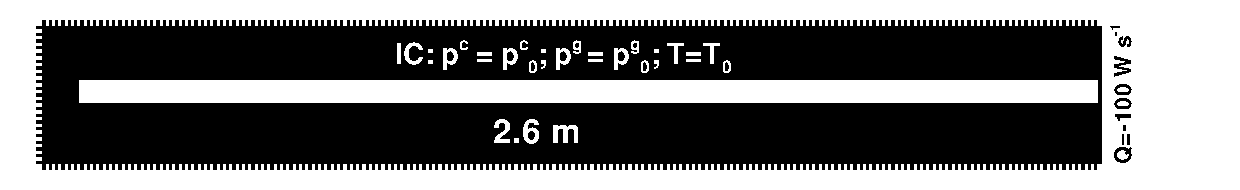
\includegraphics[height=1.25cm]{chapter_14/figures/Geo.eps}
\end{center}
\caption{Schematic of the benchmark.}
\label{Fig:HP1}
\end{figure}


\subsubsection*{Results}
In order to establish non-isothermal two-phase flow in the OpenGeoSys, we have verified numerical solutions with analytical results. Profile of water saturation $S_{\mathrm w}$, gas phase pressure $p^g$, liquid phase pressure $p^l$ and temperature $T$ are presented in Figs. \ref{Fig:HP2}, and \ref{Fig:HP4}. Numerical solutions are agreeable. Line elements have been used with variable time steps and a non uniform space discretization.
\begin{figure}[thbp]
\centerline{
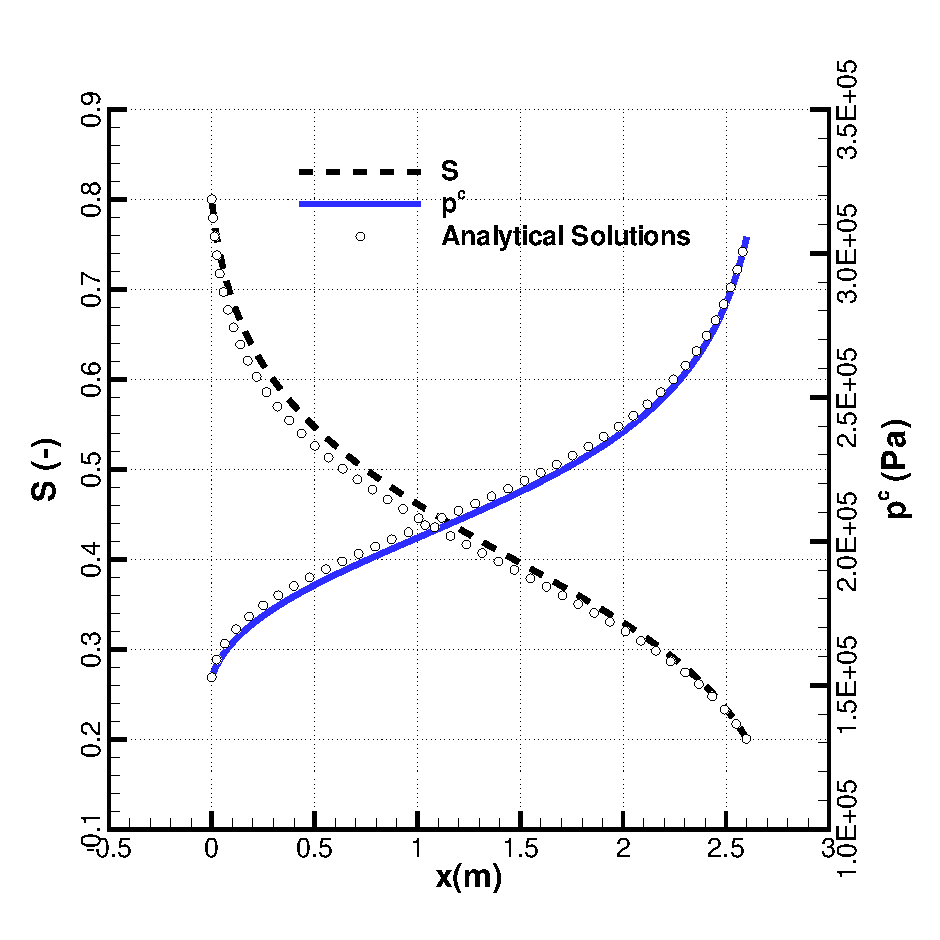
\includegraphics[height=3.0in,width=3.0in]{chapter_14/figures/S-Pc.eps}
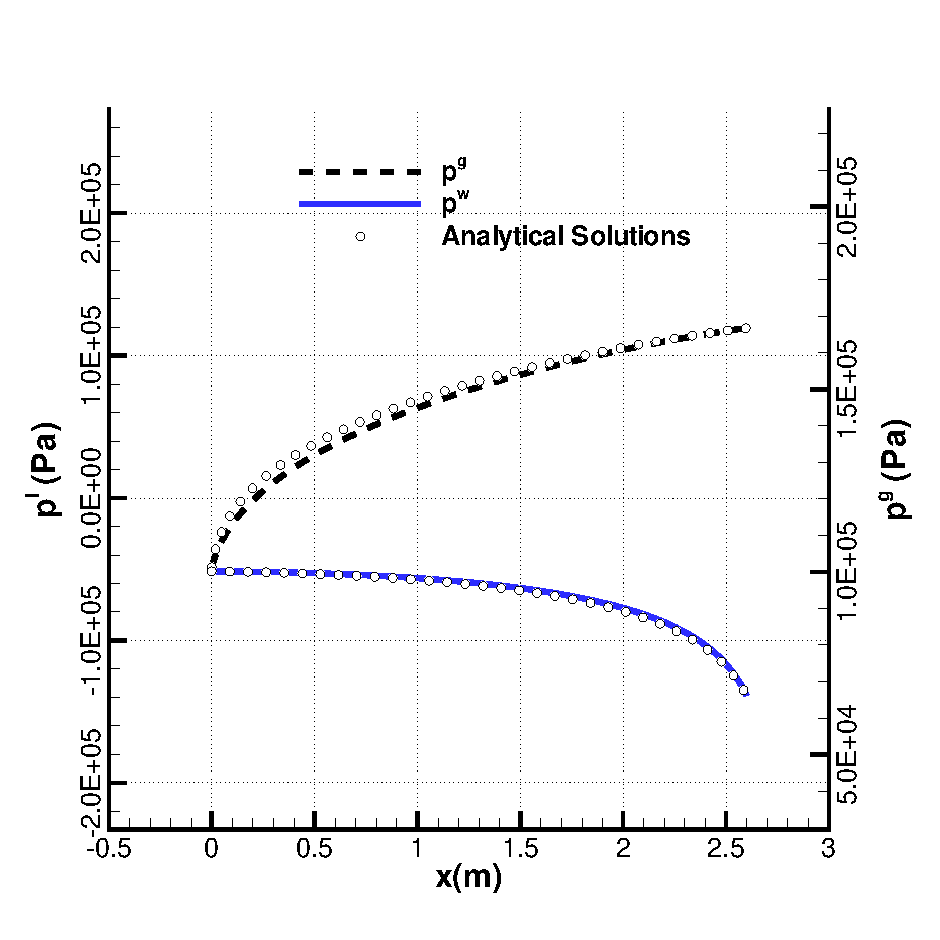
\includegraphics[height=3.0in,width=3.0in]{chapter_14/figures/Pw-Pg.eps}}
\caption{Comparison of water saturation and pressure profiles from present solution with analytical solution.}
\label{Fig:HP2}
\end{figure}
A finite element approach has been developed for the nonisothermal two-phase flow model based on the $ppT$ formulation. We used a combined monolithic/ staggered coupling scheme i.e. monolithic for the two-phase flow and staggered for the heat transport.
\begin{figure}[htb]
\begin{center}
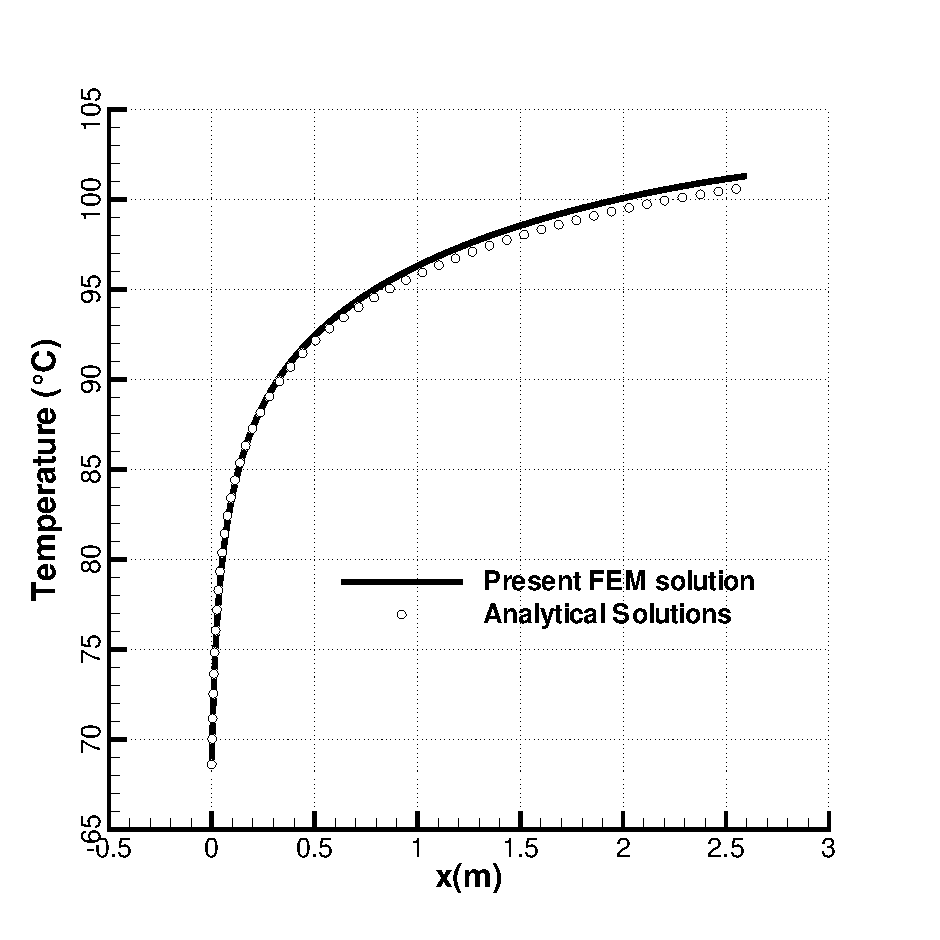
\includegraphics[height=8cm]{chapter_14/figures/Tg.eps}
\end{center}
\caption{Comparison of temperature profile from present solution with analytical solution.}
\label{Fig:HP4}
\end{figure}
\begin{table}[htbp]
\caption{Material parameters for the heat pipe problem.}
\label{tab:HP1}
\begin{tabular}{l*{4}{l}r}
\hline
\textbf{Meaning} & \textbf{Symbol} &  \textbf{Value} &  \textbf{Unit} \\
\hline
Column length & $L$ & $\mathrm m$ & $2.6$  \\
Liquid dynamic viscosity &  $\mu^l$ & $\mathrm {Pa.s}$ & $1.0\times10^{-3}$ \\
Gas dynamic viscosity & $\mu^g$ & $\mathrm {Pa.s}$ & $1.0\times10^{-5}$ \\
Liquid density &  $\rho^l$ &$\mathrm {kg.m^{-3}}$ & $1.0\times10^{3}$ \\
Permeability & $\mathbf k$ & $ \mathrm {m^2}$ & $1.0\times 10^{-13}$ \\
Porosity & $n$ & $--$ & $0.3$ \\
Residual saturation of water &  $S_{\mathrm{rl}}$ & $--$ & $0.2$ \\
Residual saturation of oil &  $S_{\mathrm{rg}}$ & $--$ & $0$ \\
Soil distribution index &  $\lambda$ & $--$ & $2.0$ \\
Capillary pressure & $p^c(S)$ & $\mathrm {Pa}$ & Brooks-Corey model\\
Relative permeability & $\kappa_{\mathrm {r\gamma}}(S)$ & $--$ & Brooks-Corey model \\ \hline
\end{tabular}
\end{table}

\subsection{DECOVALEX unsaturated test case}
DECOVALEX is an international code comparison project for the verification of thermo-hydro-mechanical (THM) and thermo-hydro-chemical (THC) numerical simulators \cite{BirEtAl:2008}.

\subsubsection*{Definition}
The original DECOVALEX-THM benchmark definition is a 2-D problem \cite{BirEtAl:2008}. For the comparison of different HM swelling models, we consider a simplified case representing a horizontal cross-section through the 2-D domain. Examined here is the isothermal HM consolidation problem with unsaturated flow.

\begin{figure}[!t]
\begin{center}
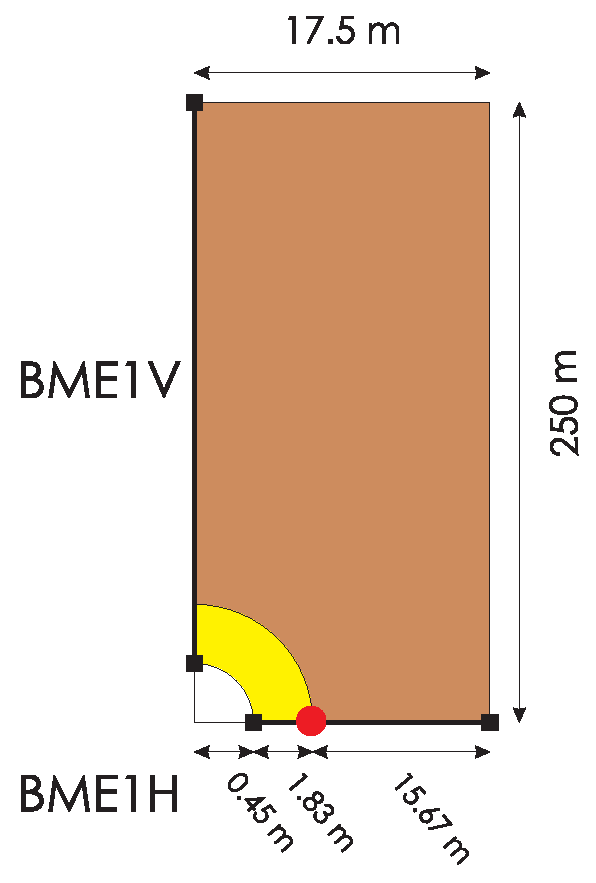
\includegraphics[width=0.3\textwidth]{chapter_14/figures/fig_14_2_15}
\end{center}
\caption{2D DECOVALEX HM definition and simplification for the benchmark exercise BME1H.}
\label{fig:thm-1D}
\end{figure}

\begin{figure}[!t]
\begin{center}
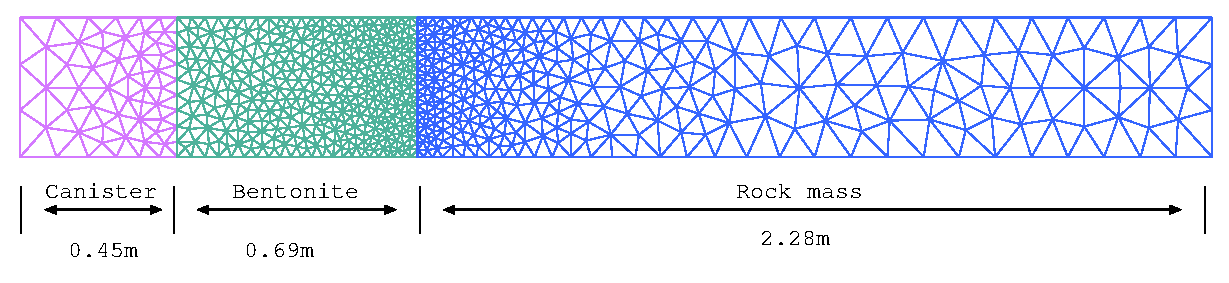
\includegraphics[width=1.0\textwidth]{chapter_14/figures/fig_14_2_16}
\end{center}
\caption{Mesh of the simplified BME1H model including canister, bentonite, and rock mass sections.}
\label{fig:thm-1Dmesh}
\end{figure}

The simplified model takes a rectangle shape. The mesh of the domain together with material types are shown in Fig. \ref{fig:thm-1Dmesh}. Fig. \ref{fig:BME1H} illustrates the definition of initial and boundary conditions for the horizontal cross-section. Observation points are set at $x=0.45\,m, \,x=1.10\,m$ to record temporal breakthrough curves. Material parameters for the rock mass and bentonite are given in Table \ref{tab:hm_rock}.

\begin{table}[!thb]
\begin{center}
\begin{tabular}{lll}
\hline
Parameter   &  Unit  & Value\\
\hline
\textit{Rock mass properties} & & \\
Density &  $kg/m3$ &  2700 \\
Young's modulus &  $GPa$ &  $35$ \\
Poisson ratio & - &  0.3 \\
Porosity & - &  0.01 \\
Saturated permeability &  $m2$  & $1.0\times10^{-17}$ \\
\\
\textit{Bentonite properties} & & \\
Density &  $kg/m3$ &  1600 \\
Young's modulus &  $MPa$ &  $317$\\
Poisson ratio & - &  0.35 \\
Saturated permeability &  $m2$  & $2.0
\times10^{-21}$ \\
\hline
\end{tabular}
\end{center}
\caption{\label{tab:hm_rock}Solid properties of different materials.}
\end{table}

\begin{figure}[!htb]
\begin{center}
%\footnotesize
\scalebox{0.8} % Change this value to rescale the drawing.
{
\begin{pspicture}(0,-1.900625)(18.579687,1.900625)
\definecolor{color7g}{rgb}{1.0,0.0,0.2}
\definecolor{color0g}{rgb}{0.4,0.4,0.4}
\definecolor{color0f}{rgb}{0.6,0.6,0.6}
\psframe[linewidth=0.04,dimen=outer,fillstyle=gradient,gradlines=2000,gradbegin=color0g,gradend=color0f,gradmidpoint=1.0](12.799687,1.0171875)(1.7796875,-1.1428125)
\psframe[linewidth=0.04,dimen=outer,fillstyle=gradient,gradlines=2000,gradbegin=color7g,gradend=color7g,gradmidpoint=1.0](3.7996874,1.0171875)(1.7596875,-1.1228125)
\psframe[linewidth=0.04,dimen=outer,fillstyle=gradient,gradlines=2000,gradbegin=blue,gradend=blue,gradmidpoint=1.0](6.4396877,1.0171875)(3.7796874,-1.1428125)
\psframe[linewidth=0.04,dimen=outer](18.539688,1.4571875)(18.519688,1.2971874)
\usefont{T1}{ptm}{m}{n}
\rput(7.403125,1.5271875){$u_y$=0, $\sigma_{xy}$=0}
\usefont{T1}{ptm}{m}{n}
\rput(7.383125,-1.6728125){$u_y$=0, $\sigma_{xy}=0$}
\usefont{T1}{ptm}{m}{n}
\rput(14,0.2471875){$u_x=0, \sigma_{xy}=0$}
\usefont{T1}{ptm}{m}{n}
\rput(13.8,-0.1){$p^l=10^6$Pa}
\usefont{T1}{ptm}{m}{n}
\rput(0.973125,0.2471875){$u_x$=0}
\usefont{T1}{ptm}{m}{n}
\rput(0.99,-0.1){$\sigma_{xy}$=0}
\usefont{T1}{ptm}{m}{n}
\rput(5.,0.24){\color{red}S0=0.65}
\usefont{T1}{ptm}{m}{n}
\rput(5.1,-0.1){\color{yellow}($p^l=-7\times10^7$Pa)}
\usefont{T1}{ptm}{m}{n}
\rput(9,-0.1728125){\color{yellow}$p^l=10^5$Pa}
\end{pspicture}
}
\end{center}
\caption{Simplified horizontal cross-section model.}
\label{fig:BME1H}
\end{figure}

The dependency of capillary pressure and relative permeability on liquid saturation for both rock and bentonite are depicted in Fig. \ref{fig:cp_cp}.

\begin{figure}[!htb]
\begin{center}
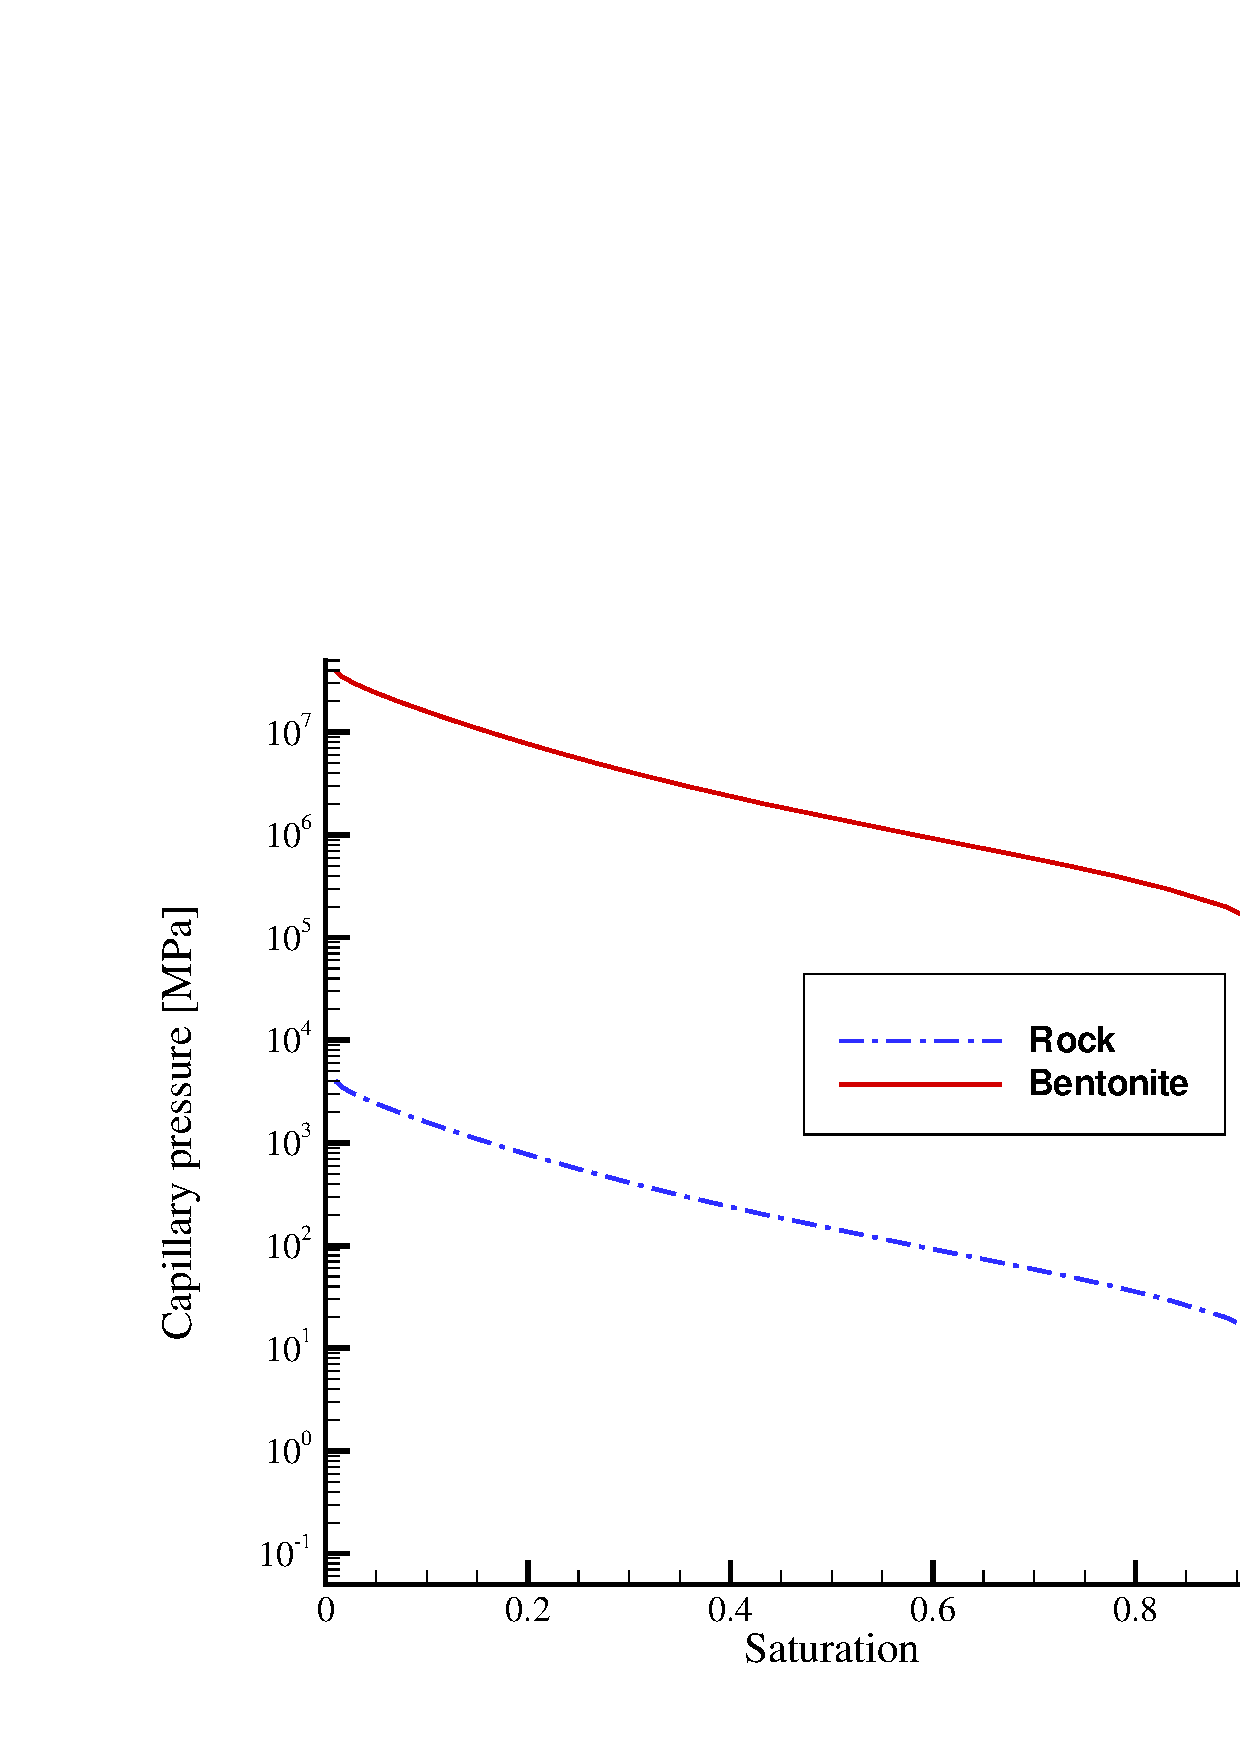
\includegraphics[width=0.49\textwidth]{chapter_14/figures/fig_14_2_18_a}
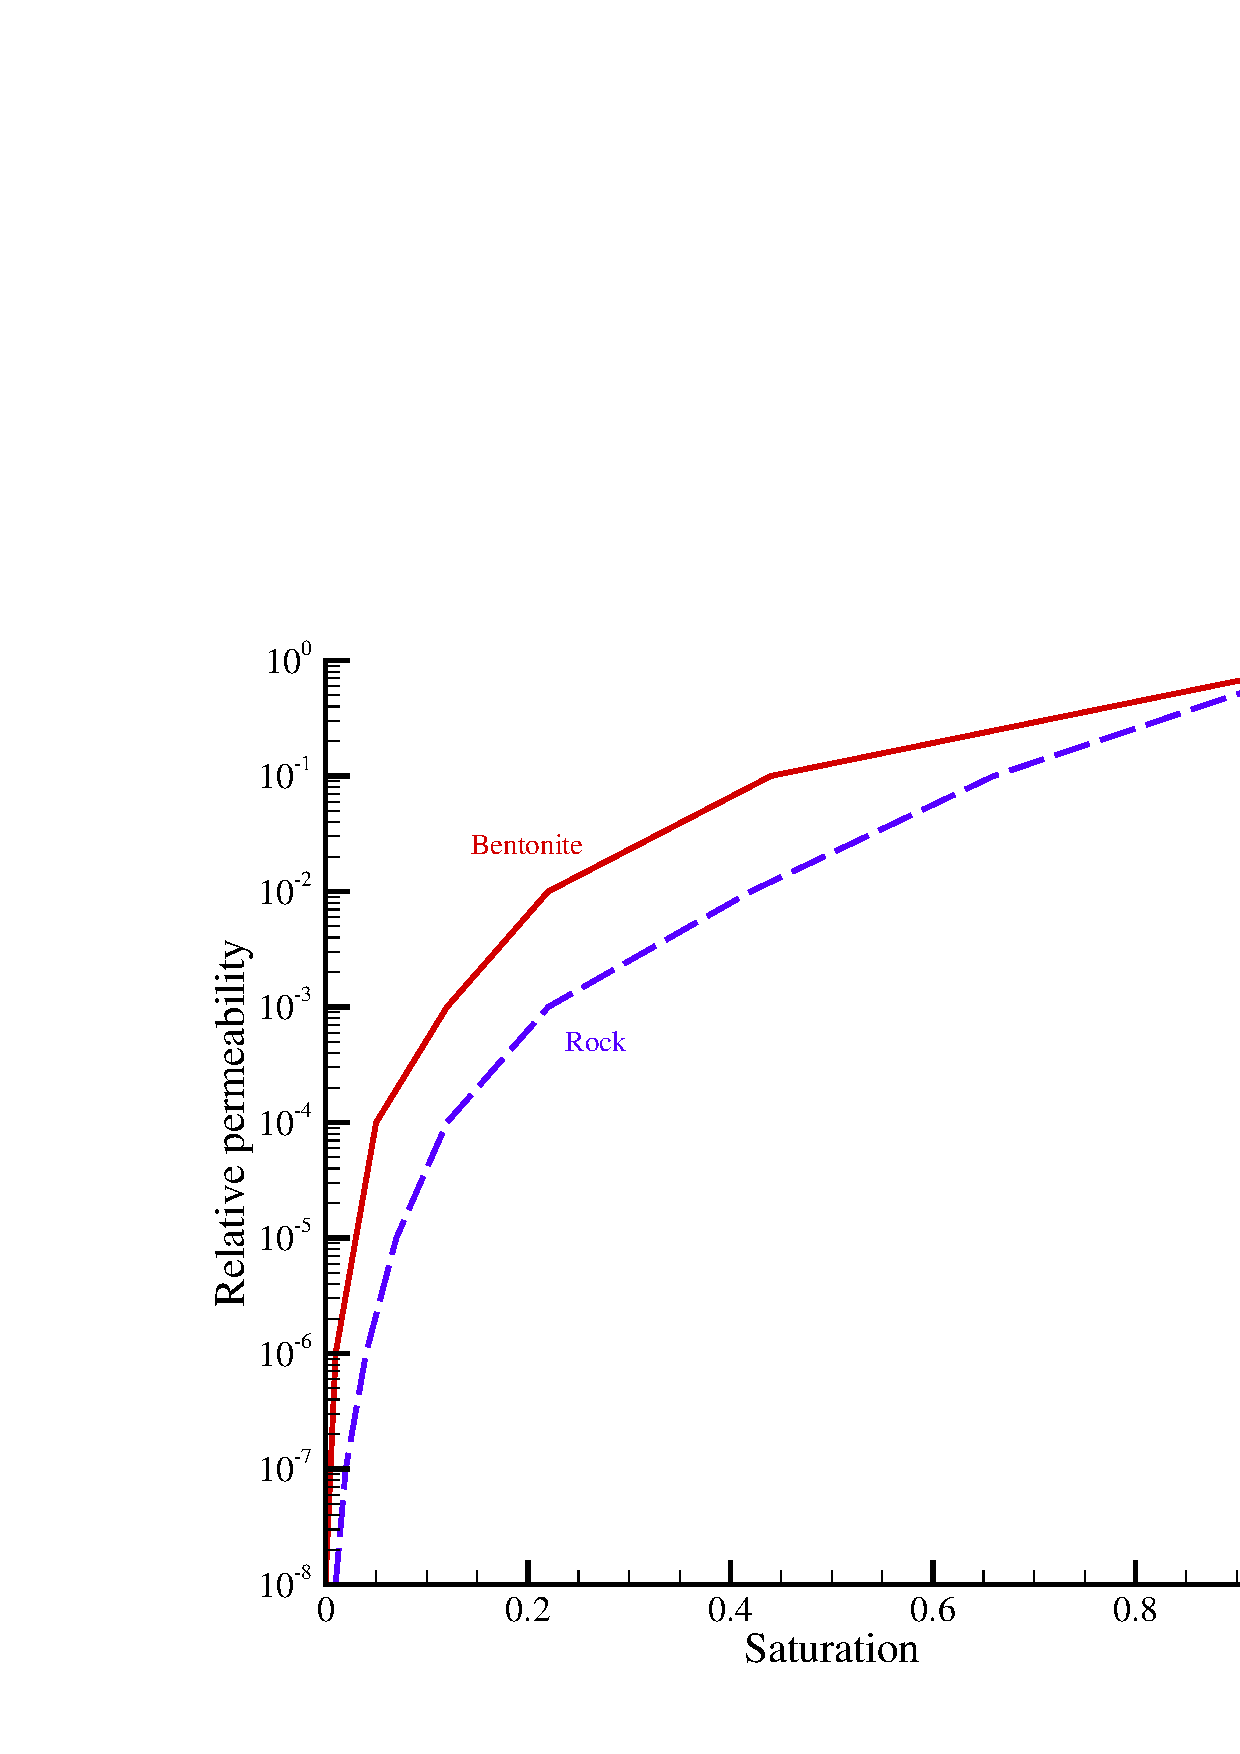
\includegraphics[width=0.49\textwidth]{chapter_14/figures/fig_14_2_18_b}
\end{center}
\caption{Capillary pressure and relative permeability functions.}
\label{fig:cp_cp}
\end{figure}

\begin{figure}[!t]
\begin{center}
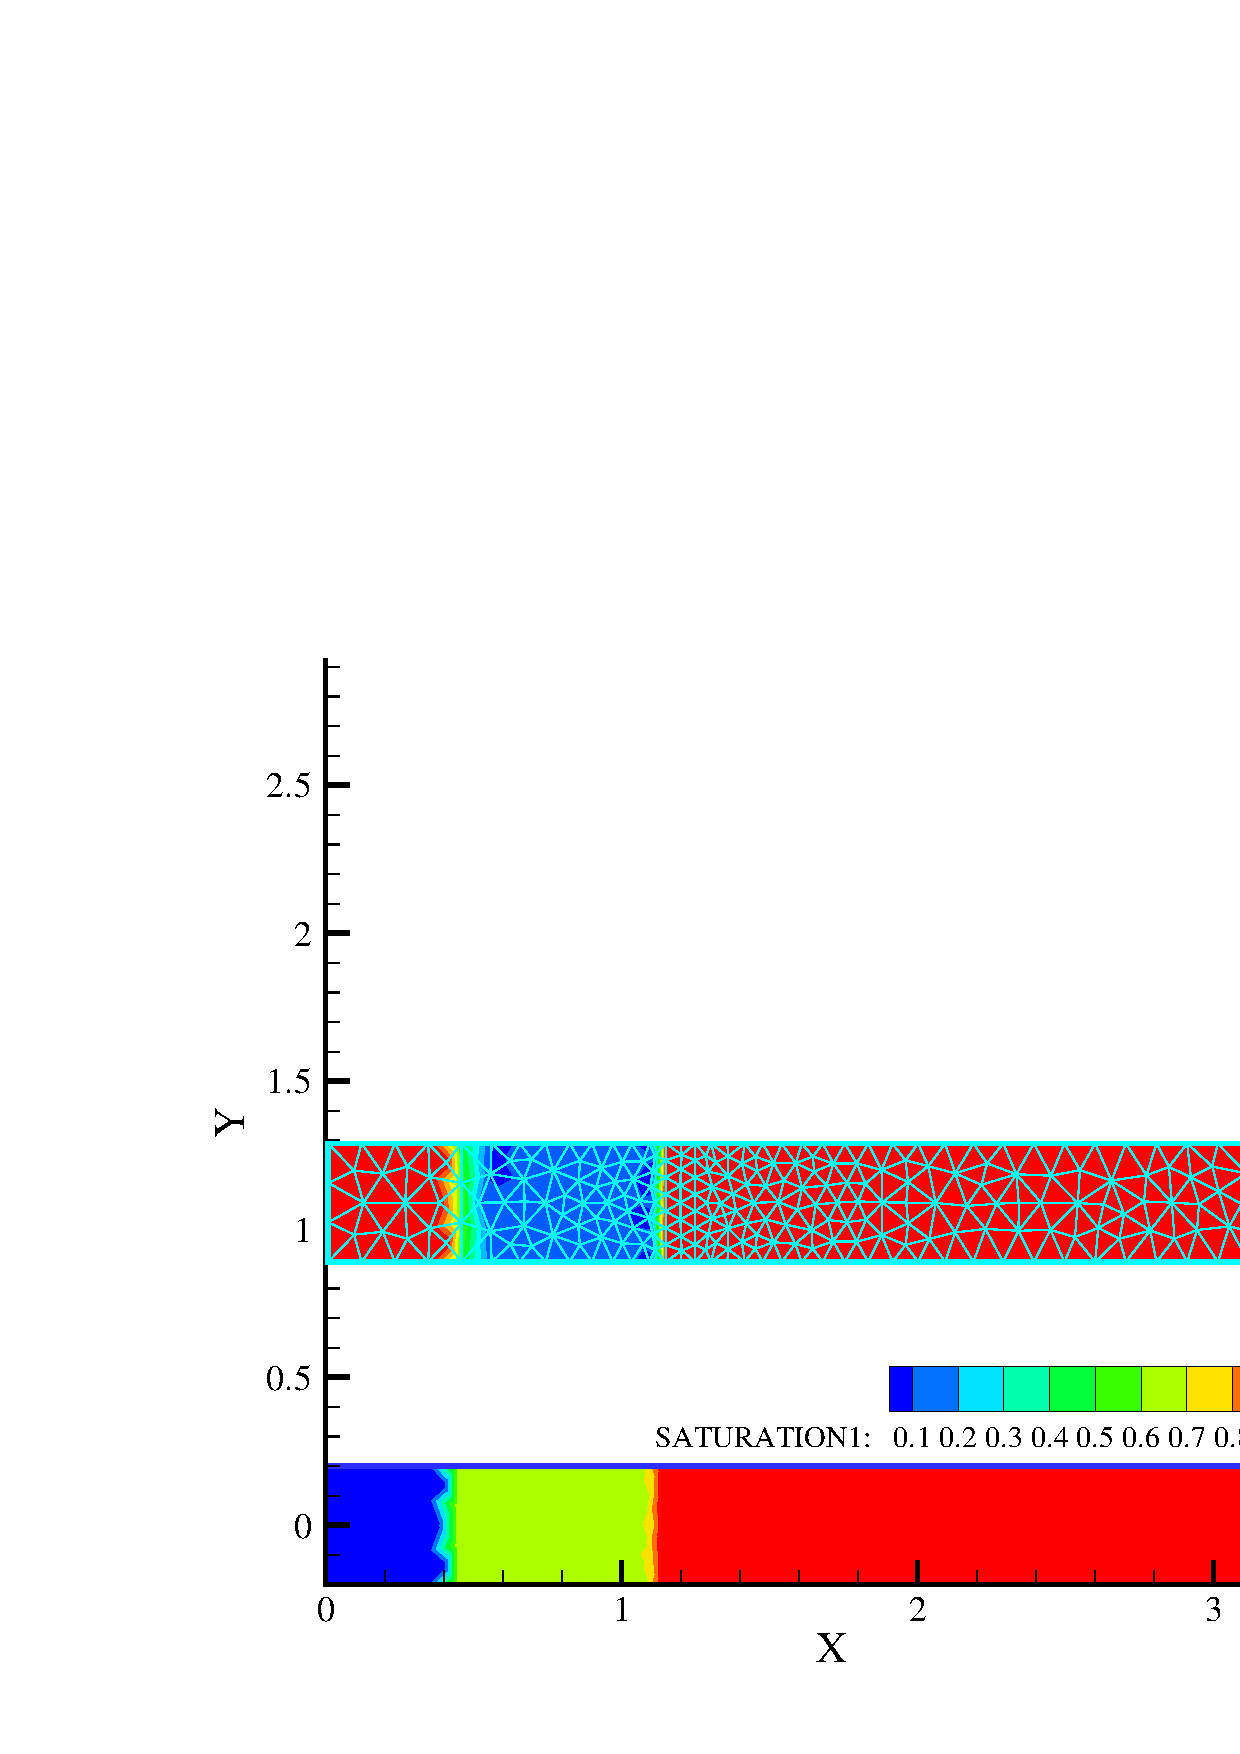
\includegraphics[width=0.7\textwidth]{chapter_14/figures/fig_14_2_19}
\end{center}
\caption{Distribution of saturation and vertical swelling stress}
\label{fig:hmswl_cont}
%\end{figure}
%\begin{figure}[!t]
\begin{center}
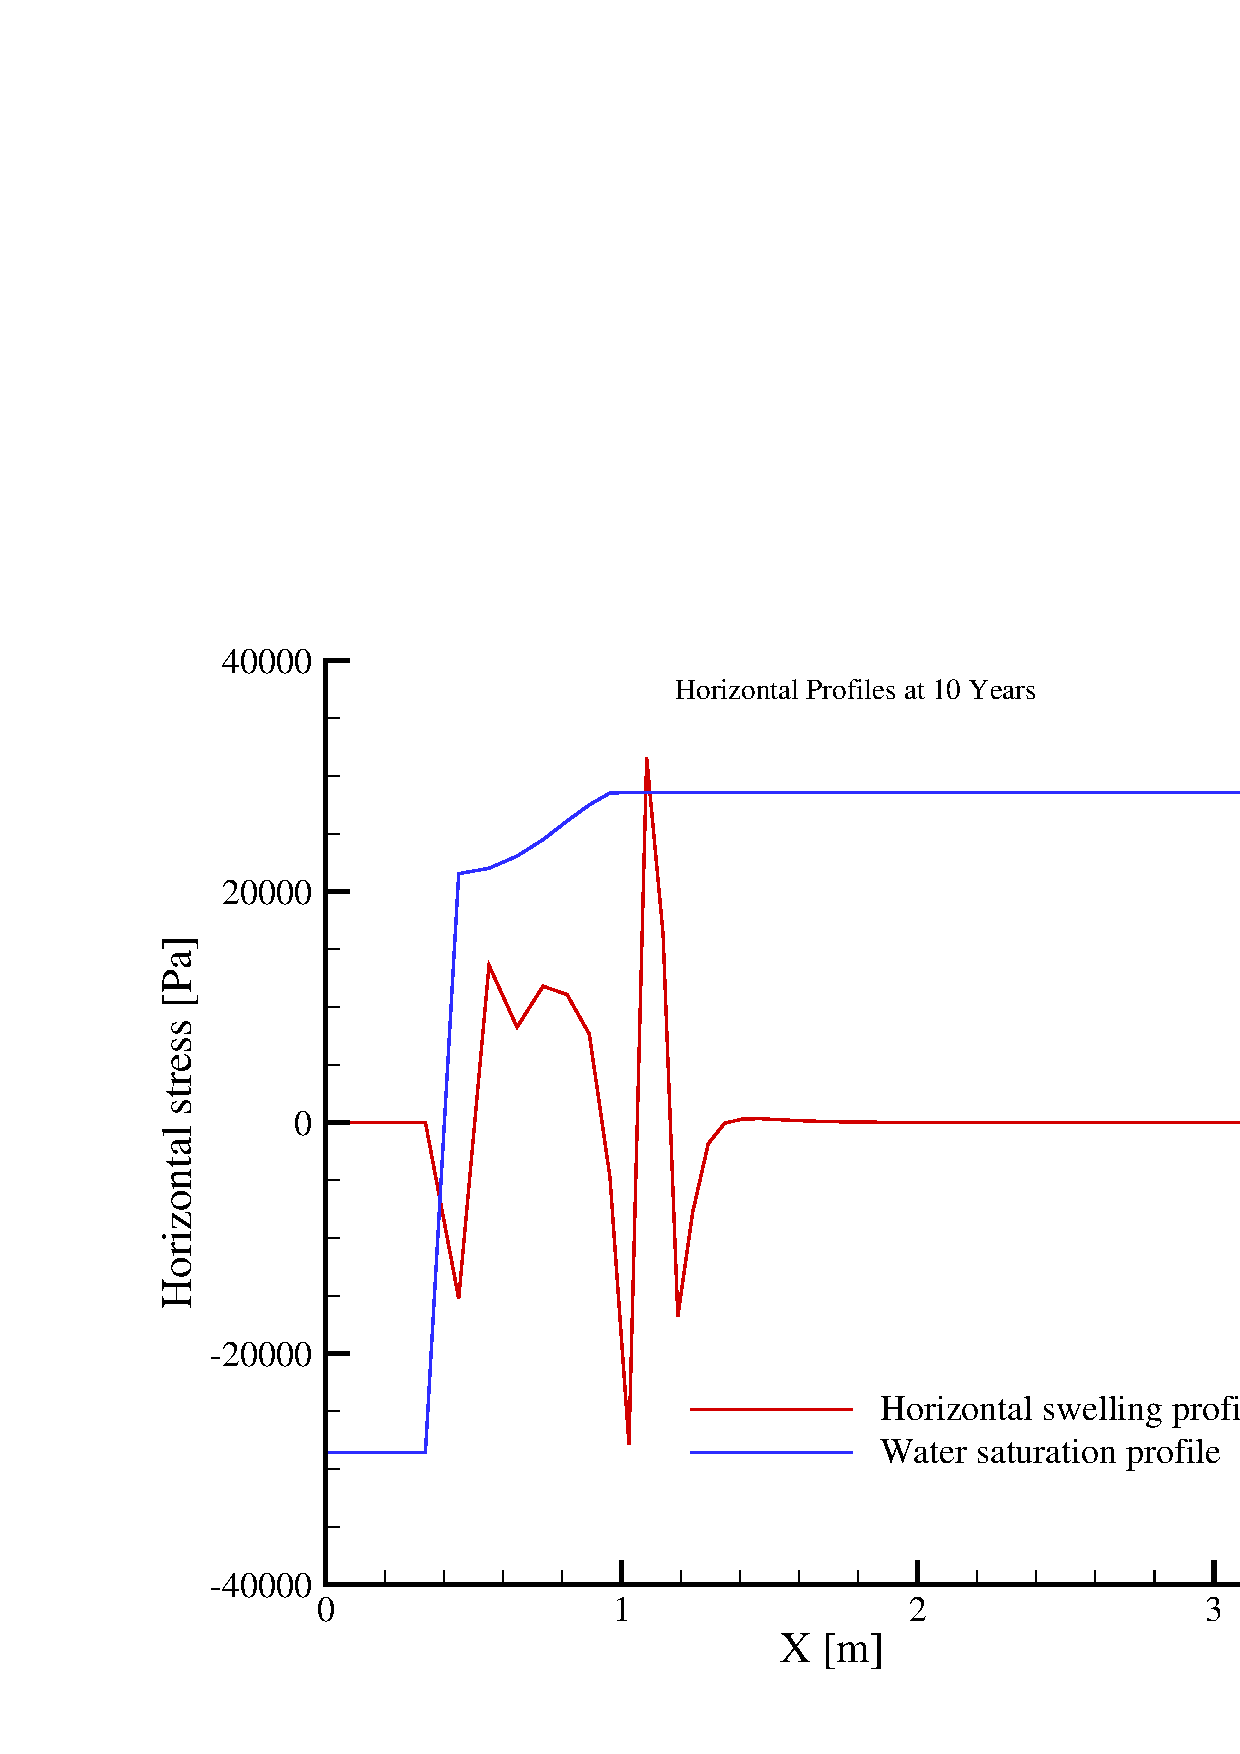
\includegraphics[width=0.49\textwidth]{chapter_14/figures/fig_14_2_20_a}
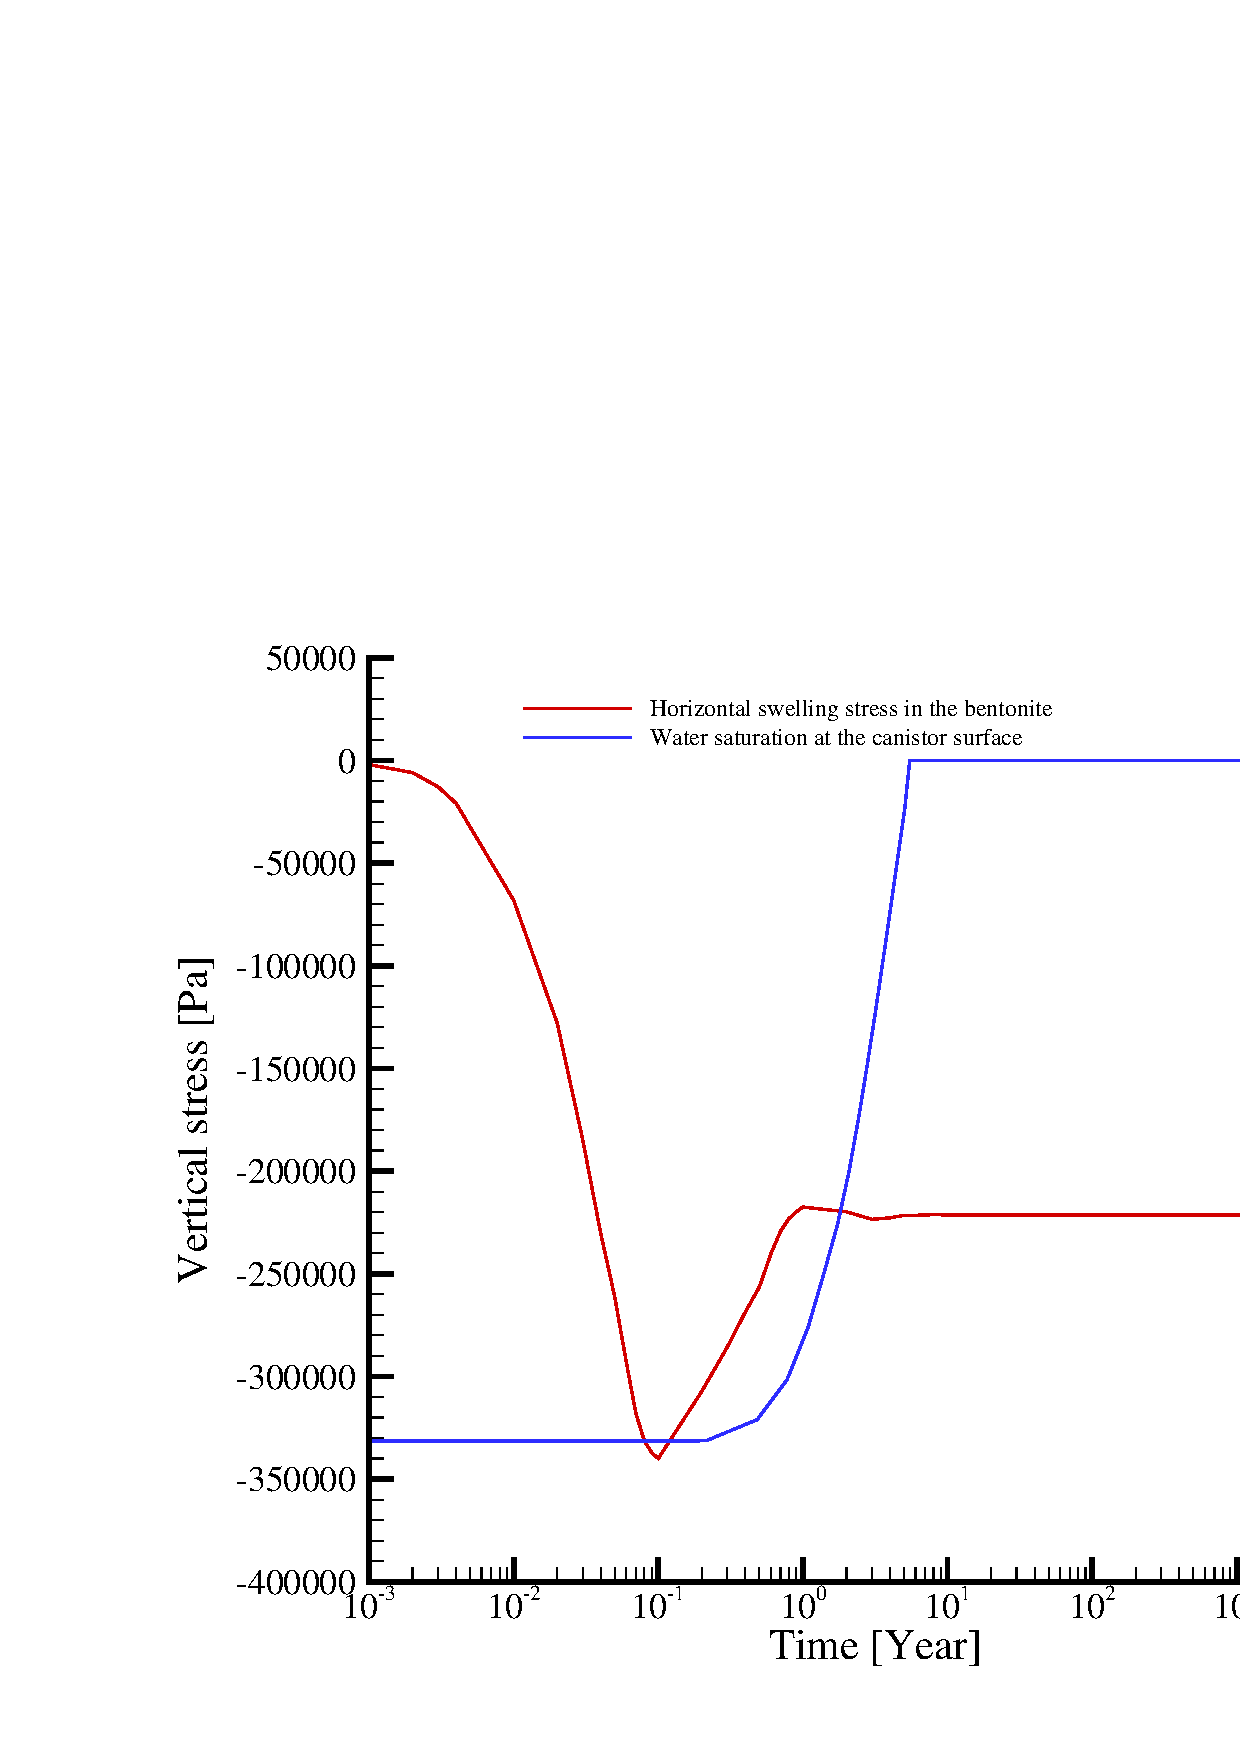
\includegraphics[width=0.49\textwidth]{chapter_14/figures/fig_14_2_20_b}
\end{center}
\caption{Horizontal profile (top) and temporal evolution at observation point (bottom) of water saturation and swelling stress}
\label{fig:deco-hm}
\end{figure}

\subsubsection*{Results}
Fig. \ref{fig:hmswl_cont} displays a contour plot of saturation and vertical swelling stress in the domain. Swelling stress in the bentonite is clearly induced by change of water saturation. Fig. \ref{fig:deco-hm} shows the simulated horizontal profiles (top) and temporal evolutions at the observation point (bottom) of water saturation and swelling stress based on the linear swelling model proposed by Rutqvist (2005) \cite{Jonny05}, which defines the increment of swelling stress to be proportional to liquid saturation increment,

\begin{equation}
\Delta \sigma ^{sw}=\beta \Delta S_w,
\end{equation}

where $\beta $ is a swelling coefficient that could be called the maximum swelling stress. As the saturation change approaches unity, swelling stress approaches $\beta $.

Fig. \ref{fig:deco-hm} shows the simulated horizontal profiles and temporal evolutions at the observation point of water saturation and swelling stress based on the linear swelling model proposed by Rutqvist (2005) \cite{Jonny05}.


%\section{Two-Phase}
\section{Two-phase consolidation}

For the two-phase system the governing equations presented in the previous sections must be expanded slightly.

\subsubsection*{Fluid mass and momentum balance}
Following the same mass balance procedure as for the single phase case, and gathering two mass balance equations, one for a wetting fluid (i.e. liquid) and one for a non-wetting (i.e. gas) fluid, we write,

\begin{equation}
\begin{split}
{{S}_{w}}\left( \frac{\phi }{{{K}_{w}}}+\frac{\alpha -\phi }{{{K}_{s}}} \right)\frac{d{{p}_{w}}}{dt}-\phi \frac{d{{S}_{nw}}}{dt}+... \\
\nabla \cdot \left\{ \frac{\mathbf{k}k_{w}^{r}}{{{\mu }_{w}}}\left( -\nabla {{p}_{w}}+{{\rho }_{w}}\mathbf{g} \right) \right\}+\alpha {{\text{S}}_{w}}\nabla \cdot \frac{\partial \mathbf{u}}{\partial t}=0
\end{split}
\label{eq:H2liq}
\end{equation}

for mass balance of the wetting fluid, subscript $w$, and,

\begin{equation}
\begin{split}
{{S}_{nw}}\left( \frac{\phi }{{{K}_{nw}}}+\frac{\alpha -\phi }{{{K}_{s}}} \right)\frac{d{{p}_{w}}}{dt}+\phi \left( 1-\frac{{{S}_{nw}}}{{{K}_{nw}}}\frac{\partial {{p}_{c}}}{\partial {{S}_{w}}} \right)\frac{d{{S}_{nw}}}{dt}+... \\
\nabla \cdot \left\{ \frac{\mathbf{k}k_{nw}^{r}}{{{\mu }_{nw}}}\left( -\nabla {{p}_{w}}-\frac{\partial {{p}_{c}}}{\partial {{S}_{w}}}\nabla {{S}_{nw}}+{{\rho }_{nw}}\mathbf{g} \right) \right\}+\alpha {{S}_{nw}}\nabla \cdot \frac{\partial \mathbf{u}}{\partial t}= 0
\end{split}
\label{eq:H2gas}
\end{equation}

for mass balance of the non-wetting fluid, subscript $nw$. In these equations, $k^{r}_{\alpha }$ is relative permeability of phase $\alpha $, $\rho _{\alpha }$ is density of phase $\alpha $, and we have chosen wetting pressure, $p_w$, and non-wetting saturation, $S_{nw}$, as primary variables in the solution scheme. Other primary variables, such as capillary pressure, $p_c$, and non-wetting pressure, $p_{nw}$, could also have been chosen with algebraic manipulation, but our benchmark example requires constant, $p_c=0$, capillary pressure for comparison with an anylitical solution. This is not possible, of course, if $p_c$ is a primary variable. Any viable permeability saturation function may be chosen for the example, we use the Brooks-Corey function.

For the numerical solution, storage due to two different fluids with two different compressibilities and densities is handled implicitly with solution of the above equations. For the analytical solution, we must define an effective compressibility as a function of fluid saturation and properties of each fluid. For immiscible fluids without penetrating bubbles, two compressible materials behave as resistors in series with respect to bulk modulus, thus the effective modulus is

\begin{equation}
\frac{1}{{{K}_{f}}}=\frac{{{S}_{w}}}{{{K}_{w}}}+\frac{{{S}_{nw}}}{{{K}_{nw}}}.
\end{equation}

\subsubsection*{Solid momentum balance}

As with the single phase case, balance of linear momentum is defined by,

\begin{equation}
\frac{\partial {{\sigma }_{ij}}}{\partial {{x}_{j}}}+{{F}_{i}}=0,
\end{equation}

but now the body force is a function of two fluids, $F=\rho _m \text{g}$ for the mixture density $\rho _m =\phi (S_w \rho _w + S_{nw} \rho _{nw}) + (1-\phi )\rho _s$, and insertion of the elastic consitutive law yields for solid displacement,

\begin{equation}
\frac{\partial }{\partial {{x}_{j}}}\left[ G\frac{\partial {{u}_{i}}}{\partial {{x}_{j}}}+\left( \lambda +G \right)\frac{\partial {{u}_{j}}}{\partial {{x}_{i}}}-\alpha \bar{p}{{\delta }_{ij}} \right]+{{F}_{i}}=0,
\end{equation}

where \textit{mean} fluid pressure is defined as $\bar{p}=S_wp_w + S_{nw}p_{nw}$.

\subsubsection*{FEM solution scheme}
For the two-phase simulations, the two fluid balance equations are solved in a single global equation, with an iterative coupling to the solid balance equation. 

%-------------------------------------------------------------------------
%-------------------------------------------------------------------------

\subsection{Terzaghi consolidation: Two-phase}
\subsubsection*{Definition}
For this comparison, we may utilize the same analytical solution as was done for the single phase case in the previous section, although the solution must represent the mean fluid pressure $\bar{p}=S_wp_w + S_{nw}p_{nw}$, for the final relationship,

\begin{equation}
\frac{\bar{p}\left( z,t \right)}{\bar{p}_0}=\left\{ 1.0-{{\left( \frac{L-z}{L} \right)}^{2}}-\frac{32}{{{\pi }^{3}}}\left[ \sum\limits_{m=0}^{\infty }{\frac{{{\left( -1 \right)}^{m}}}{{{\left( 2m+1 \right)}^{3}}}\exp \left[ -{{\psi }^{2}}ct \right]\cos \left[ \psi \left( L-z \right) \right]} \right] \right\},
\end{equation} 

with pressure generation defined in the same manner,

\begin{equation}
{{\bar{p}}_{0}}=\frac{{{L}^{2}}}{2c}\left( {{B}_{v}}{{{\dot{\sigma }}}_{z}} \right),
\end{equation}

but where the uniaxial Skempton coefficient, ${B}_{v}$, must be defined (see Table \ref{terz:tab1}) based upon the effective fluid modulus. Fluid properties are then defined for two separate fluids (Table \ref{terz:tab4})

\begin{table}[!t]
\begin{center}
\begin{tabular}{lccc}
\hline\noalign{\smallskip}
Property & Symbol & Unit & Value \\
\noalign{\smallskip}\hline\noalign{\smallskip}
\textit{Wetting fluid properties} &          &        & \\
Bulk modulus   & $K_{w}$       & $GPa$       & $2.933$ \\
Density        & $\rho _{w} $  & $kg/m^3$    & $997.05$ \\
Viscosity      & $\mu _{w} $   & $Pa\dot s$  & $8.9008\times 10^{-4}$ \\
Saturation     & $S_{w}$       & $-$         & $0.8$ \\
\\
\textit{Non-wetting fluid properties} &               &               &  \\
Bulk modulus   & $K_{nw}$        & $GPa$       & $1.187$ \\
Density        & $\rho _{nw} $   & $kg/m^3$    & $997.05$ \\
Viscosity      & $\mu _{nw} $    & $Pa\dot s$  & $8.9008\times 10^{-4}$ \\
Saturation     & $S_{nw}$        & $-$         & $0.2$ \\
\noalign{\smallskip}\hline
\end{tabular}
\end{center}
\caption{Two-phase fluid properties.}
\label{terz:tab4}
\end{table}

\begin{figure}[!tbh]
\begin{center}
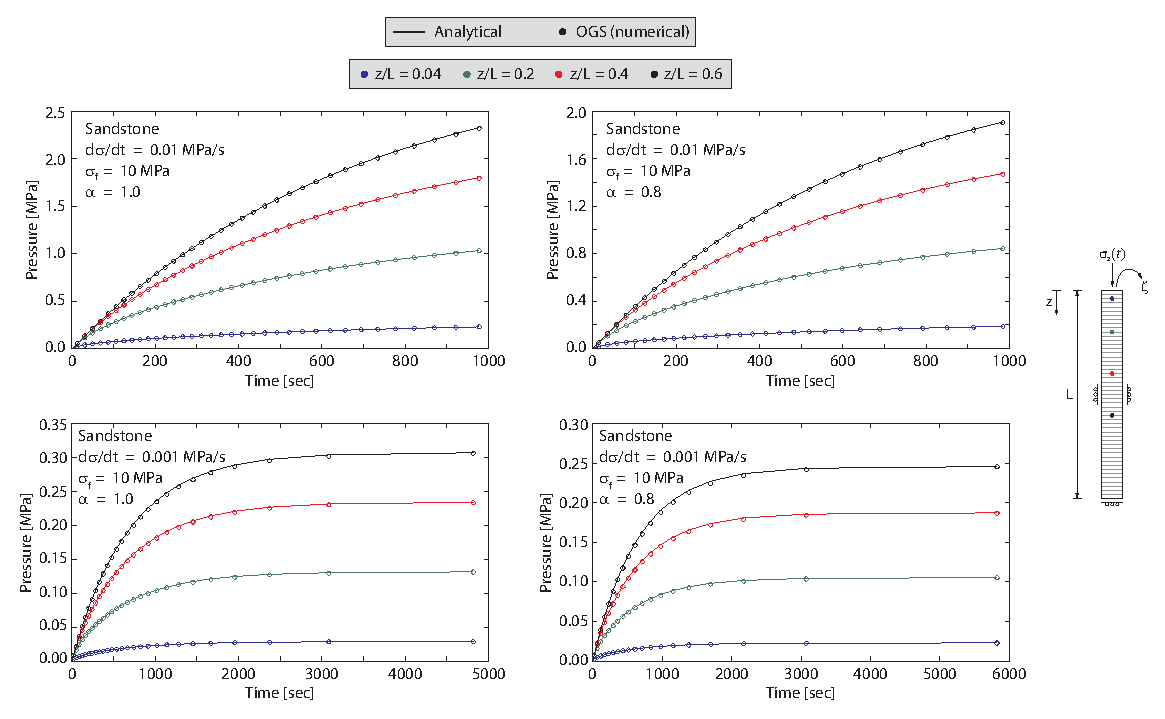
\includegraphics[width=1.0\textwidth]{chapter_14/figures/fig_14_3_21}
\end{center}
\caption{Sandstone solutions.}
\label{terz:h2msand}
%\end{figure}
%\begin{figure}[!tbh]
\begin{center}
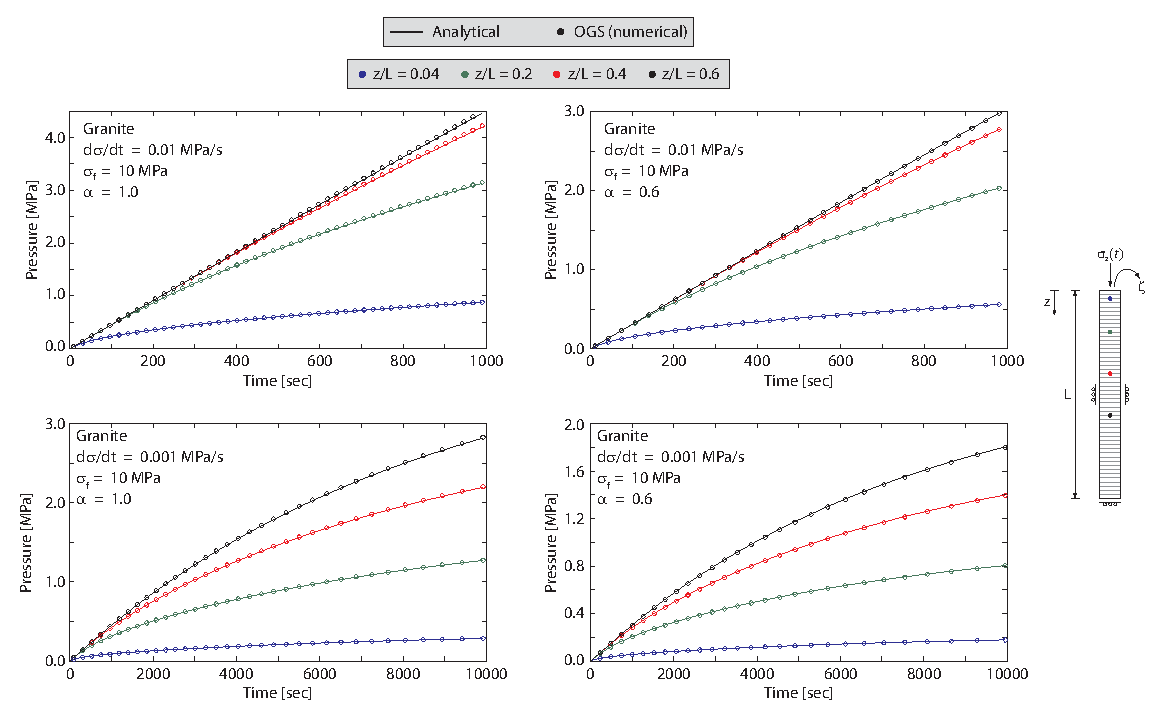
\includegraphics[width=1.0\textwidth]{chapter_14/figures/fig_14_3_22}
\end{center}
\caption{Granite solutions. Here, a porosity of 0.06 is used to ensure stability for the incompressible grain simulations (an adjustment that is not needed for compressible grains, but is used there also to maintain consistency).}
\label{terz:h2mgranite}
\end{figure}

\subsubsection*{Results}
Initially the column is at zero pressure and is saturated uniformly with both fluids ($Sw=0.8$) and we apply $p_c=0$ and $k^{r}_{w}=k^{r}_{nw}=0.5$. Note that we utilize a different compressibility for each fluid in order to exercise both fluid balance equations, with the analytical solution obtained using the \textit{effective} fluid modulus, and with the \textit{effective} modulus having an identical value to the single fluid modulus, $2.27 GPa$, used above in the single phase case.

Results are shown in Figs. \ref{terz:h2msand} and \ref{terz:h2mgranite} for sandstone and granite (see Table \ref{terz:tab2}) for incompressible and compressible grains. With reference to the staggered stability criterion discussed in the HM problem above, because we are examining incompressible grains here the solution becomes unstable for granite. Therefore, an alternate value of porosity (0.06) is utilized (in the granite simulations) to ensure stability, which results in $B_v<0.5$. Such an adjustment is not required when compressible (real) grains are used, but is utilized none-the-less for comparison with the incompressible grain solution. All results are ideally accurate. 

Time steps are adaptively controlled with a tolerance based on the rate of pressure change over a time step. Such a scheme is capable of ensuring accuracy in HM or H2M problems. Note the importance of the tolerance in Fig. \ref{terz:res1}.

\subsection{Invarient stress: Flow and storage in a compressible medium}

It is also possible, and sometimes useful, to test two-phase storage and pressure dissipation in a deformable media at invarient stress. This test guarantees accurate implementation of fluid storage within the mass matrix (time derivative term) of the fluid mass balance PDE. 

\subsubsection*{Definition}
We utilize the same problem as above, but now no stress is applied and no mechanical equilibrium performed. The analytical solution may be derived from the Carslaw and Jaeger \cite{Carslaw:59} solution for heat dissipation within a solid slab,

\begin{equation}
\bar{p}\left( z,t \right)=\frac{4{{p}_{0}}}{\pi }\sum\limits_{m=0}^{\infty }{\left\{ \frac{1}{2m+1}\sin \left[ z\left( \frac{\left( 2m+1 \right)\pi }{2L} \right) \right]\exp \left[ -ct{{\left( \frac{\left( 2m+1 \right)\pi }{2L} \right)}^{2}} \right] \right\}},
\end{equation}

where $\bar{p}_0$ is initial mean pressure within the column.

\begin{figure}[!b]
\begin{center}
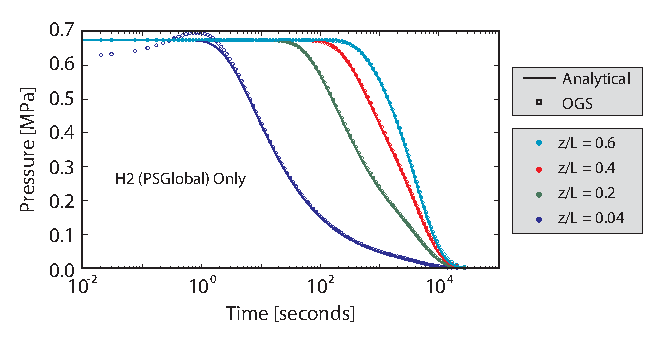
\includegraphics[width=0.7\textwidth]{chapter_14/figures/fig_14_3_23}
\end{center}
\caption{Two-phase flow with mechanical storage.}
\label{terz:h2}
\end{figure}

\subsubsection*{Results}
Results are shown in Fig. \ref{terz:h2}. We note that with an appropriate mixing rule for storage in the two phase formulation, the result is ideal.  Very small values of time and $z$ can produce inaccuracies; however, this will always be the case, barring a very small mesh discretization.
\subsection{Cam-Clay consolidation with swelling}
As before, equations \ref{eq:H2liq} and \ref{eq:H2gas} define the fluid system. In this example, however, we choose a numerical solution in OpenGeoSys that accomodates pressure variables in the solution vector. Both equations are therefore algebraically manipulated so that the primary variables to solve for are now the capillary pressure, $p_c$, and the non-wetting pressure, $p_{nw}$,

\begin{equation}
\phi {{\rho }_{w}}\frac{\partial {{S}_{w}}}{\partial {{p}_{c}}}\frac{d{{p}_{c}}}{dt}+{{\rho }_{w}}{{S}_{w}}\nabla \cdot \frac{d\mathbf{u}}{dt}+\nabla \cdot \left[ {{\rho }_{w}}\frac{\mathbf{k}k_{w}^{r}}{{{\mu }_{w}}}\left( -\nabla {{p}_{nw}}+\nabla {{p}_{c}}+{{\rho }_{w}}\mathbf{g} \right) \right]={{Q}_{w}}
\end{equation}

\begin{equation}
\begin{split}
%\begin{align}
  & -\phi {{\rho }_{nw}}\frac{\partial {{S}_{w}}}{\partial {{p}_{c}}}\frac{d{{p}_{c}}}{dt}+\phi \left( 1-{{S}_{w}} \right)\left( \frac{\partial {{\rho }_{nw}}}{\partial {{p}_{nw}}}\frac{d{{p}_{nw}}}{dt}+\frac{\partial {{\rho }_{nw}}}{\partial {{p}_{c}}}\frac{d{{p}_{c}}}{dt} \right)+ \\ 
 & \text{          }\left( {{\rho }_{w}}{{S}_{w}}+{{\rho }_{nw}}\left( 1-{{S}_{w}} \right) \right)\nabla \cdot \frac{d\mathbf{u}}{dt}+\nabla \cdot \left[ {{\rho }_{nw}}\frac{\mathbf{k}k_{nw}^{r}}{{{\mu }_{nw}}}\left( -\nabla {{p}_{nw}}+{{\rho }_{nw}}\mathbf{g} \right) \right]={{Q}_{nw}} \\ 
%\end{align}
\end{split}
\end{equation}

where in this case we assume that solid grains are incompressible. 

As in Section 14.2, swelling stress is based on the linear swelling model proposed by Rutqvist (2005) \cite{Jonny05}, which defines the increment of swelling stress to be proportional to liquid saturation increment,

\begin{equation}
\Delta \sigma ^{sw}=\beta \Delta S_w,
\end{equation}

where $\beta $ is a swelling coefficient that could be called the maximum swelling stress. As the saturation change approaches unity, swelling stress approaches $\beta $.

\subsubsection*{Definition}
Fig. \ref{fig_aximodel} shows the axi-symmetric model domain for the confined swelling test as well as the initial and boundary conditions for the two-phase flow consolidation problem with hydraulic and fluid properties are given in Table \ref{tab:hydromat}. The parameters of the elasto-plastic swelling model are given in Table \ref{tab:pls} for Cam-Clay plasticity.

\begin{figure}[!tbh]
\centering
\scalebox{0.5} % Change this value to rescale the drawing.
{
\begin{pspicture}(0,-8)(17.45797,8)
\psframe[linewidth=0.04,dimen=outer](10,7.5)(7,-7.5)
\usefont{T1}{ptm}{m}{n}
\rput(8.526719,0.1696875){
\begin{minipage}{0.12\textwidth}
{\color{blue}
\begin{align*}
&p^c=84.6\mbox{MPa}\\
&p^g=0.1\mbox{MPa}
\end{align*}
}
{\color{red}
\begin{align*}
&\sigma_x=0.1\mbox{MPa}\\
&\sigma_y=0.1\mbox{MPa}\\
&\sigma_z=0.1\mbox{MPa}\\
&\sigma_{xy}=0\\
&\sigma_{yz}=0\\
&\sigma_{zx}=0
\end{align*}
}
\end{minipage}
}
\usefont{T1}{ptm}{m}{n}
\rput{90.0}(6.5,-6)
{\rput(6.5,0.6696875){{\color{blue}${\partial p^c}/{\partial x}=0,\, {\partial p^g}/{\partial x}=0$},{\color{red}$\,u_x=0,\, \sigma_{xy}=0$}}}
\usefont{T1}{ptm}{m}{n}
\rput{90.0}(12,-11.5)
{\rput(12,0.6696875){{\color{blue}${\partial p^c}/{\partial x}=0,\, {\partial p^g}/{\partial x}=0$},{\color{red}$\,u_x=0,\, \sigma_{xy}=0$}}}
\usefont{T1}{ptm}{m}{n}
\rput(8.757343,8){{\color{blue}${\partial p^c}/{\partial y}=0,\, p^g=0.1\mbox{MPa}$},{\color{red}$\,u_y=0,\, \sigma_{xy}=0$}}
\usefont{T1}{ptm}{m}{n}
\rput(8.757343,-8){{\color{blue}$p^c=0,\, p^g=0.1\mbox{MPa}$},{\color{red}$\,u_y=0,\, \sigma_{xy}=0$}}
\end{pspicture}
}
\caption{Model set-up with initial and boundary conditions.}
\label{fig_aximodel}
\end{figure}

\begin{table}[!htb]
\centering
\begin{tabular}{lll}
\hline\noalign{\smallskip}
Meaning & Value & Unit \\
\hline
Liquid density, $\rho _{w}$ & $1000$ & $kg/m^3$\\
Liquid viscosity, $\mu_w$ &$10^{-3}$ & $Pa\,s$\\
Gas density,  $\rho _{nw}$ & Clapeyron equation & $kg/m^3$\\
Gas viscosity, , $\mu _{nw}$ &$1.8\times10^{-5}$ & $Pa\,s$\\
Intrinsic permeability, $k$ & $0.6\times10^{-20}$ & $m^2$\\
Porosity, $\phi $ & $0.4$ & $m^3/m^3$ \\
Media properties for liquid: &  & \\
\textit{Relative permeability} & Power law $k_{w}^r=S_e^3$  & \\
Residual saturation & 0 &--- \\
Maximum saturation & 1 &--- \\
\textit{Water retention} & van Genuchten  & \\
Exponential index, $m$ & 0.42 &--- \\
Air entry pressure, $p_0$& 62 &$MPa$ \\
Relative permeability of gas, $k_{nw}^r$ & $5.103\times10^{-12}\left[e(1-S^l)\right]^{4.3}$ & $e$, void ratio\\
\hline
\end{tabular}
\caption{Hydraulic properties} %\footnotesize
\label{tab:hydromat}
\end{table}

\begin{table}[!htb]
\centering
\begin{tabular}{lrl}
\hline\noalign{\smallskip}
Parameter & Value & Unit \\
\hline
Slope of the critical state line, $M$ & $1.5$ & ---\\
Virgin compression index, $\lambda_p$ & $1.5$ & ---\\
Swelling/recompression index, $\kappa$ & $0.1$ & ---\\
Initial preconsolidation pressure, $p_c$& $8.0$ & $MPa$\\
Initial void ratio, $e$ & $0.7$ & $--$\\
Poisson ratio & $0.4$ & ---\\
Initial ($s=0$) elastic slope for $1+e-p$, $\kappa_{i0}$& $0.01$ & ---\\
Initial ($\sigma=0$) elastic slope for $1+e-s$, $\kappa_{s0}$& $0.25$ & ---\\
Minimum bulk modulus, $K_{min}$ & $10$ &$MPa$\\
First parameter for $\kappa_s$, $\alpha_{ss}$ & $-0.03$ & $MPa^{-1}$\\
Second parameter for $\kappa_s$, $\alpha_{sp}$ & $-0.1609$ & ---\\
Parameter for $\kappa_i$, $\alpha_{i}$ & $-0.003$ & $MPa^{-1}$\\
Reference mean stress, $p_{ref}$ & $0.1$ & $MPa$\\
\hline
\end{tabular}
\caption{Plasticity parameters for the Cam-Clay model} %\footnotesize
\label{tab:pls}
\end{table}

\subsubsection*{Results}
Fig. \ref{fig:S_top} shows the temporal evolution of water saturation on the bottom of the sample between OpenGeoSys and Code-Bright.

\begin{figure}[!thb]
\begin{center}
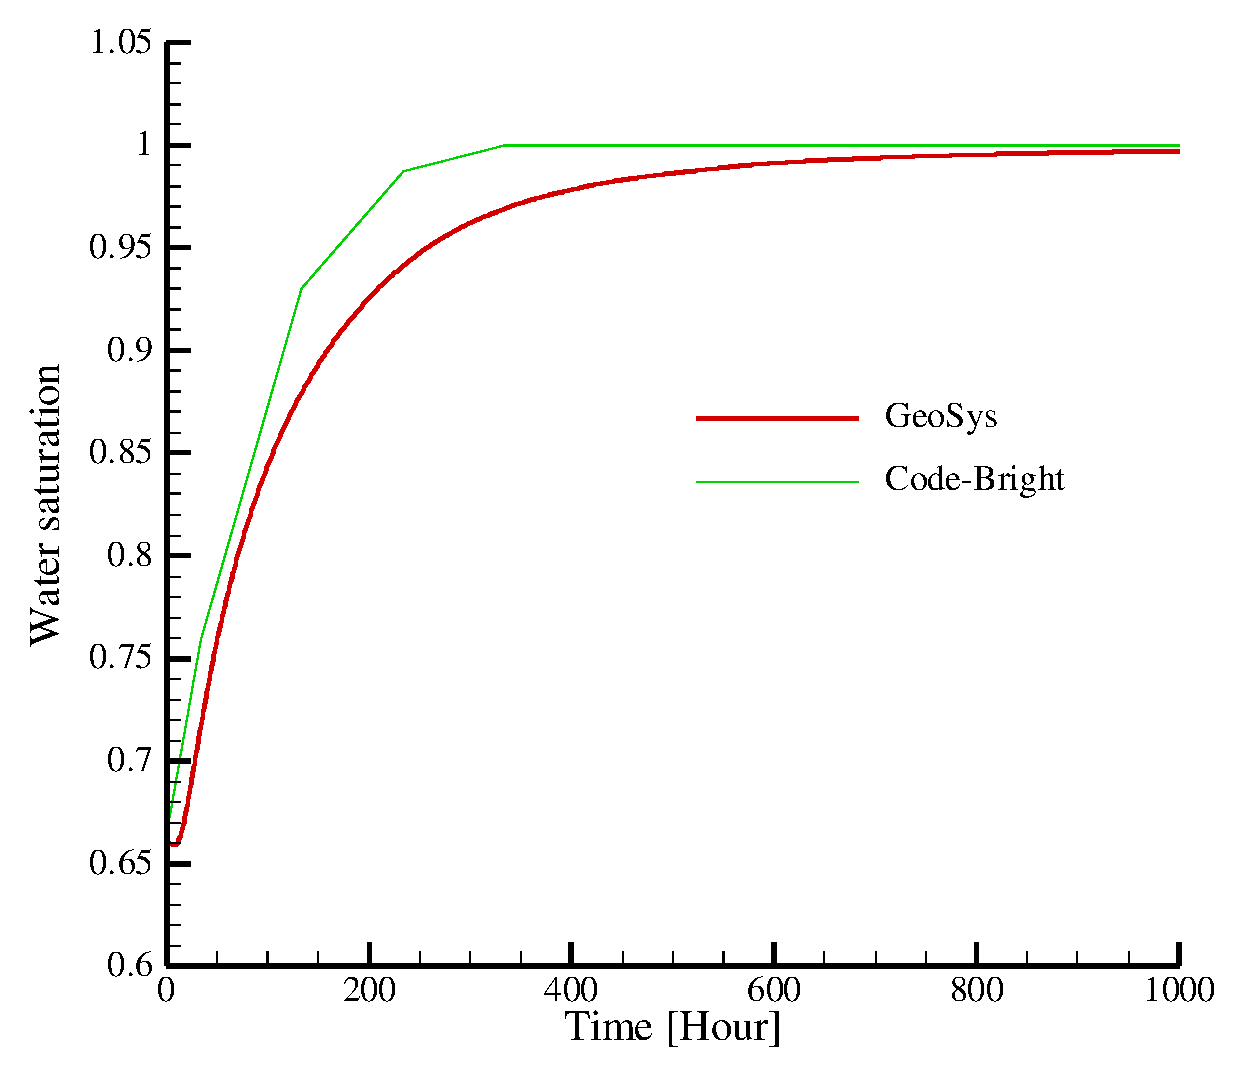
\includegraphics[width=0.7\textwidth]{chapter_14/figures/fig_14_3_25}
\end{center}
\caption{Water saturation evolution at the sample bottom.}
\label{fig:S_top}
\end{figure}


%\section{Discrete Fractures}
\section{Flow and mechanics in discrete fracture-matrix rock systems}

%-------------------------------------------------------------------------
%-------------------------------------------------------------------------

\subsection{Hydro-mechanical response of a single fracture within a rock matrix (2D)}

\subsubsection*{Definition}
This example is a fluid injection problem into a single discrete fracture surrounded by an impermeable rock matrix in two-dimensional space and validates the proposed lower-dimensional interface elements with local enrichments for the nonlinear, coupled HM problem. 
The test case is designed to mimic the semi-analytical similarity solution available in \cite{Wijesinghe1986}, which has been used to verify numerical codes such as ROCMAS II \cite{Noorishad1992}, GEOCRACK \cite{Swenson1995}, and FEHM \cite{Bower1997}. Test parameters are referred to those of  \cite{Bower1997}.
The solution is available based on the following assumptions:
\begin{enumerate}
\item  The fluid compressibility is small compared to the compliance of the fracture aperture under normal effective stress. (This is valid for liquid saturated fractures.)
\item  Fluid flow in a fracture is laminar flow between parallel surfaces.
\item  Fracture deformation is not hysteretic.
\item  The gradient in aperture along the fracture is small. There is no shear deformation of the fracture or the fracture does not dilate when sheared.
\item  Displacements parallel to the fracture are negligible everywhere within the rock mass.
\end{enumerate}

Figure \ref{fig:ex_hm_single_problem} shows a sketch of the calculation model. The major fracture lies horizontally in the middle of an impermeable rock block.  
The fracture is subjected to a uniform in-situ stress $\stress_{yy}=50$ MPa normal to the fracture. Initially, fracture aperture is uniformly $b_0 = 1.0 \cdot 10^{-2}$ mm and fluid pressure is $p_0=11.0$ MPa along the fracture. At time $t=0^+$, fluid is injected at the left-most edge of the fracture (in the form of constant boundary pressure, $p=11.9$ MPa) and a sudden increase of pressure in the fracture results.
%
The injection pressure induces elastic fracture opening and a subsequent increase of fracture permeability and storage capacity. 
%
\begin{figure}[!tbh]
\centering
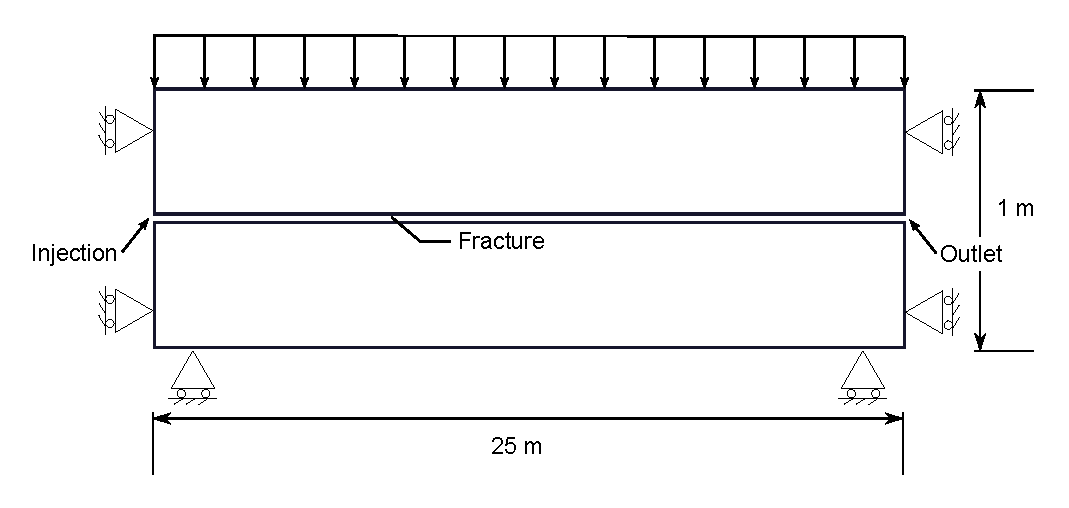
\includegraphics[width=120mm]{chapter_14/figures/fig_14_4_26}
\caption{Fluid injection into a discrete fracture-rock matrix system.}
\label{fig:ex_hm_single_problem}
\end{figure}

\begin{table}[!htb]
\centering
\caption{Model parameters}
\label{tbl:ex_hm_single_setting}
\begin{tabular}{llrr}
\toprule
Symbol & Parameter & Value & Unit \\
\midrule
\multicolumn{4}{l}{\textit{Fluid}}  \\ 
$\rho^l$ & Density & 1000.0 & $kg \cdot m^{-3}$ \\  
$\mu$ & Viscosity & 0.001 & $Pa \cdot s$ \\  \\ 
\multicolumn{4}{l}{\textit{Porous medium}}  \\  
$\rho^s$ & Density & 2716.0 & $kg \cdot m^{-3}$ \\ 
$S_s$ & Specific storage & $1.0\cdot 10^{-10}$ & ${Pa}^{-1}$ \\ 
$k$ & Permeability & $1.0\cdot 10^{-21}$ & $ m^2 \cdot s^{-1}$ \\ 
$\phi$ & Porosity & 0.1  & $ \%$ \\ 
$E$ & Young's modulus & 60 & $ GPa$ \\ 
$\nu$ & Poisson ratio & 0.0 & $-$ \\ 
$\alpha$ & Biot constant & 1.0 & $-$ \\  \\
\multicolumn{4}{l}{\textit{Fracture}}  \\  
$b_0$ & Initial aperture & $1.0\cdot 10^{-5}$ & $m$ \\ 
$S_s$ & Specific storage & 0.0 & $Pa^{-1}$ \\ 
$k_n$ & Joint normal stiffness & 100 & $GPa \cdot m^{-1}$ \\ 
$k_s$ & Joint shear stiffness & 100 & $GPa \cdot m^{-1}$ \\ 
$\alpha$ & Biot constant & 1.0 & $-$ \\ 
\bottomrule
\end{tabular}
\end{table}

\subsubsection*{Semi-analytical solution}
Wijesinghe \cite{Wijesinghe1986} derived the ordinal differential equation with the dimensionless aperture $w$. The semi-analytical solution can be obtained by solving the equation as an initial value problem using the fourth order Runge-Kutta method. For details, please refer to the original work \cite{Wijesinghe1986}. %Initial values are $w1(0)$, $w2(0)$. However, $Q(0)$, which is used for $w1(0)$ is still unknown. Thus, an iterative method with changing $Q(0)$ needs to be executed to satisfy a boundary condition $w2( \infty )=1$. \cite{Wijesinghe1986} suggests using $w2(10)=1$.

\subsubsection*{Numerical solution}
Boundary fluid pressure is fixed at $t=0^+$ to 11.9 MPa at the left and 11 MPa at the right. Line elements with local enrichment were used to represent the discrete fracture and quadrilateral elements for surrounding rock matrix. Very fine vertical discretization is required near the fracture, i.e. $\Delta y$=0.001 m. The time step is selected as 10 s and a Newton-Raphson iteration is utilized to solve the nonlinear equation. 

\subsubsection*{Results}
Simulation results are presented in Figure \ref{fig:ex_hm_single_result} for pressure and fracture aperture profile along the fracture. When fluid is injected, the fracture aperture is instantaneously opened to nearly 1.9 $\cdot 10^{-2}$ mm at the injection point ($x = 0$ m). With time, this fracture opening behavior gradually propagates toward the right-most, low-pressure edge of the fracture. Linear constitutive laws dictate a linear variation in fracture aperture relative to fluid pressure.
%discussion
Figure \ref{fig:ex_hm_single_result} shows good agreement between the  numerical method and the semi-analytical solution.

\begin{figure}[!tbh]
\centering
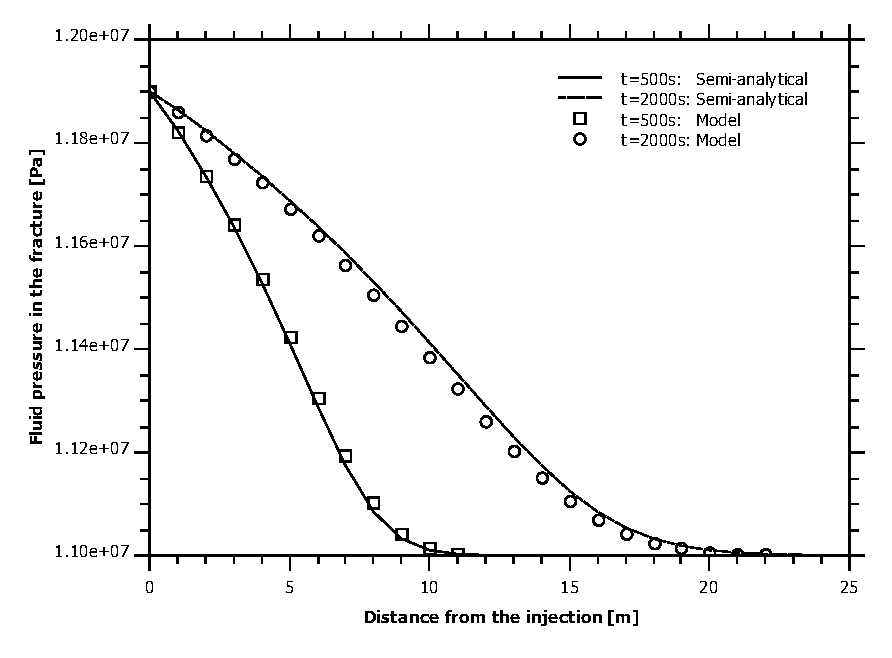
\includegraphics[width=100mm]{chapter_14/figures/fig_14_4_27_a}
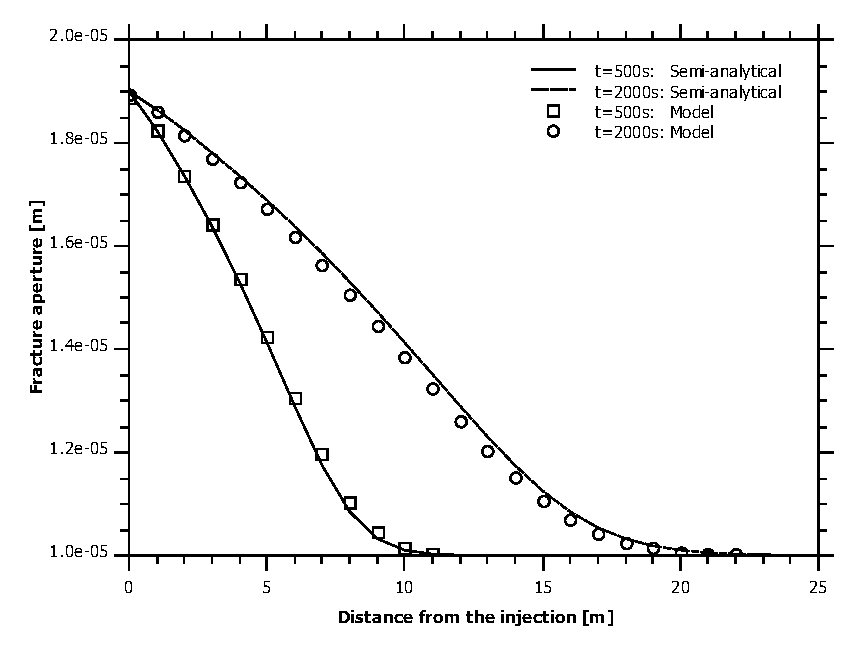
\includegraphics[width=100mm]{chapter_14/figures/fig_14_4_27_b}
\caption{Profile along the fracture: pressure (left) and aperture (right).}
\label{fig:ex_hm_single_result}
\end{figure}



%.........................................................................
